\documentclass{templateNote}
\usepackage{pgfplots}

\pgfplotsset{compat=1.18}
\definecolor{morado}{RGB}{127,0,255}
\newcolumntype{g}{>{\columncolor{green!50}}c}

\begin{document}

\imagenlogoU{img/LogoElNube.png}
\linklogoU{https://github.com/MarceloPazPezo}
\linkQRDoc{https://github.com/MarceloPazPezo/MyRepo/blob/main/Icinf/Semestre\%207/Investigación\%20de\%20Operaciones/Programacion_Lineal/Programacion-Lineal.pdf}
\titulo{Certamen 1}
\asignatura{Investigación de Operaciones}
\autor{
Marcelo Paz
}
\vDoc{1.6.1}
% Metadatos del PDF
\title{[\asignatura]-\titulo}
\author{\autor}
\portada
\margenes % Crear márgenes

\section*{Diagrama de flujo: Programación Lineal}
\begin{figure}[H]
    \centering
    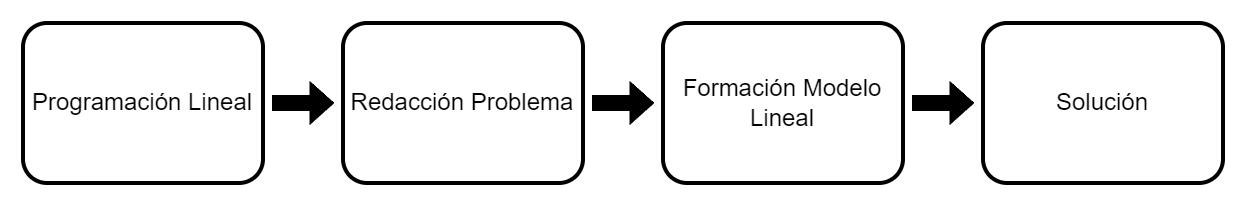
\includegraphics[width=1\textwidth]{diagram/Fig1.png}
\end{figure}

\section{Modelo de Programación Lineal}
\begin{equation*}
    \begin{aligned}
        \left(
            \begin{array}{ccc}
                \text{Max} \\
                \text{o} \\
                \text{Min} \\
            \end{array}
        \right) \quad & Z = c_1x_1 + c_2x_2 + \ldots + c_nx_n \\
        &\left.
            \begin{array}{llll}
                \text{s.a} \quad & a_{11}x_1 + a_{12}x_2 + \ldots + a_{1n}x_n \left(
                    \begin{array}{ccc}
                        \leq \\
                        = \\
                        \geq \\
                    \end{array}
                \right)  b_1 \\
                & a_{21}x_1 + a_{22}x_2 + \ldots + a_{2n}x_n \left(
                    \begin{array}{ccc}
                        \leq \\
                        = \\
                        \geq \\
                    \end{array}
                \right) b_2 \\
                & \vdots \\
                & a_{m1}x_1 + a_{m2}x_2 + \ldots + a_{mn}x_n \left(
                    \begin{array}{ccc}
                        \leq \\
                        = \\
                        \geq \\
                    \end{array}
                \right) b_m \\
            \end{array}
        \right\} \text{Restricciones} \\
        & x_1, x_2, \ldots, x_n \geq 0
    \end{aligned}
\end{equation*}    

Donde:
\begin{itemize}
    \item $Z$ es la función objetivo.
    \item $c_1, c_2, \ldots, c_n$ son los coeficientes de Costo.
    \item $a_{ij}$ son los coeficientes Tecnologicos.
    \item $b_i$ son Constantes RHS(Right Hand Side).
    \item $x_j$ son las Variables de Decisión.
\end{itemize}

\newpage
\subsection*{Problema 1: Método gráfico}
Un colegio va a realizar un paseo. En total participarán 400 personas entre alumnos y profesores. Se requiere contratar buses para el traslado de dichas personas. Al llamar a una empresa de transportes se obtiene la siguiente información: La empresa dispone de 8 buses con 40 asientos y 10 buses con 50 asientos. Para el día del paseo habrá 9 choferes disponibles. El costo de arriendo es de \$ 30.000 por cada bus de 40 asientos y de \$40.000 por cada bus de 50 asientos. Antes de contratar los buses, el Director del colegio debe decidir cuántos buses de cada tipo les conviene arrendar para que el arriendo resulte lo más económico posible. Cuál será la decisión de menor costo?

\subsubsection*{Variables de Decisión:}
\begin{itemize}
    \item $x_1$ = Cantidad de buses de 40 asientos por contratar.
    \item $x_2$ = Cantidad de buses de 50 asientos por contratar.
\end{itemize}

\subsubsection*{Función Objetivo:}
\begin{equation*}
    \begin{aligned}
        \text{Min} \quad & Z = 30000x_1 + 40000x_2 \\
        \text{s.a} \quad & 40x_1 + 50x_2 \geq 400 \\
        & x_1 \leq 8 \\
        & x_2 \leq 10 \\
        & x_1 + x_2 \leq 9 \\
        & x_1, x_2 \geq 0
    \end{aligned}
\end{equation*}

\subsubsection*{Solución por método gráfico:}
\begin{figure}[H]
    \centering
    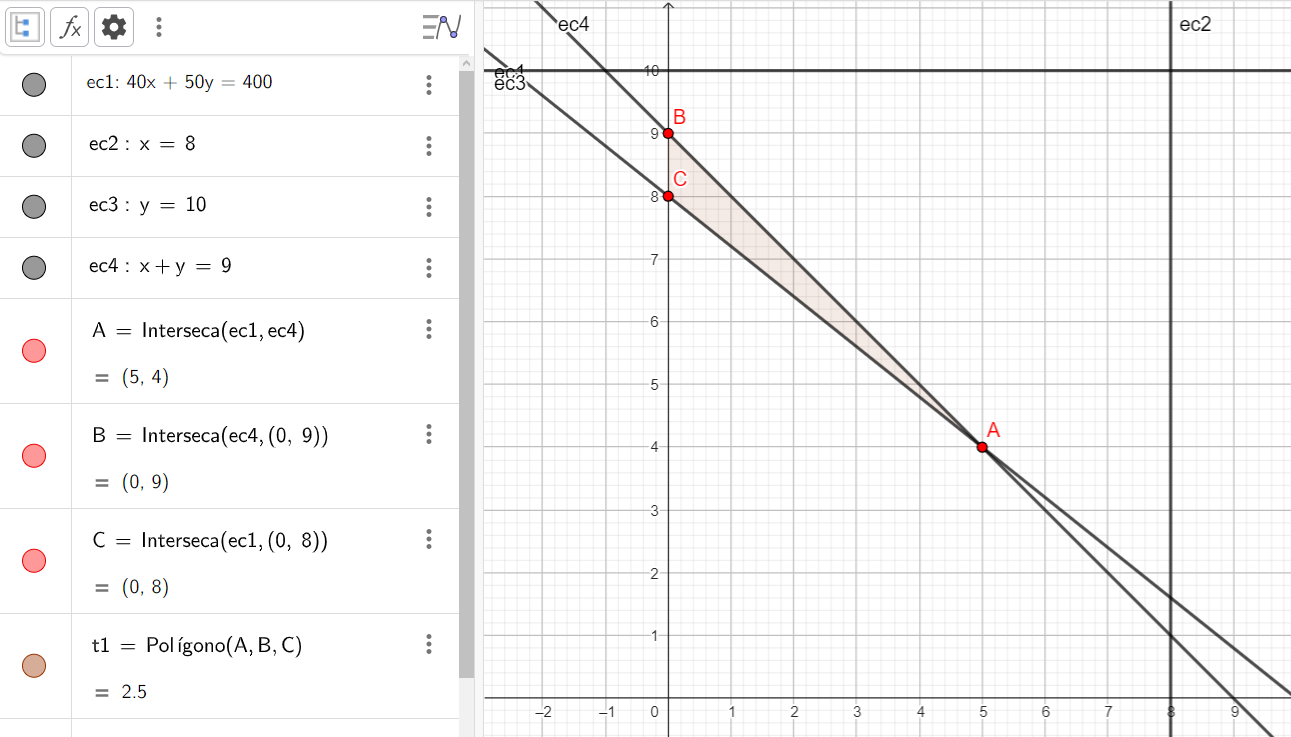
\includegraphics[width=0.7\textwidth]{img/Problema1Grafica.png}
\end{figure}
\begin{center}
    \begin{tabular}{|c|c|c|}
        \hline
        \textbf{Vertice ($x_1,x_2$)} & Z &  \\ \hline
        A(5, 4) & 310000 & * \\ \hline
        B(0, 9) & 360000 & \\ \hline
        C(0, 8) & 320000 & \\ \hline
    \end{tabular}
\end{center}

\newpage
\subsection*{Problema 2:}
\subsubsection*{Función Objetivo: Restricción redundante}
\begin{equation*}
    \begin{aligned}
        \text{Min} \quad & Z = 2x_1 - 6x_2 \\
        \text{s.a} \quad & x_1 + x_2 \leq 5 \quad &\textbf{No Activa} \\
        & x_2 \leq 3 \quad &\textbf{Activa} \\
        & x_1 - x_2 \leq 1 \quad &\textbf{No Activa} \\
        & x_1 \geq 1 \quad &\textbf{Activa} \\
        & x_1 - 2x_2 \leq 2 \quad &\textbf{No Activa} \\
        &x_1,x_2 \geq 0
    \end{aligned}
\end{equation*}

\subsubsection*{Solución por método gráfico:}
\begin{figure}[H]
    \centering
    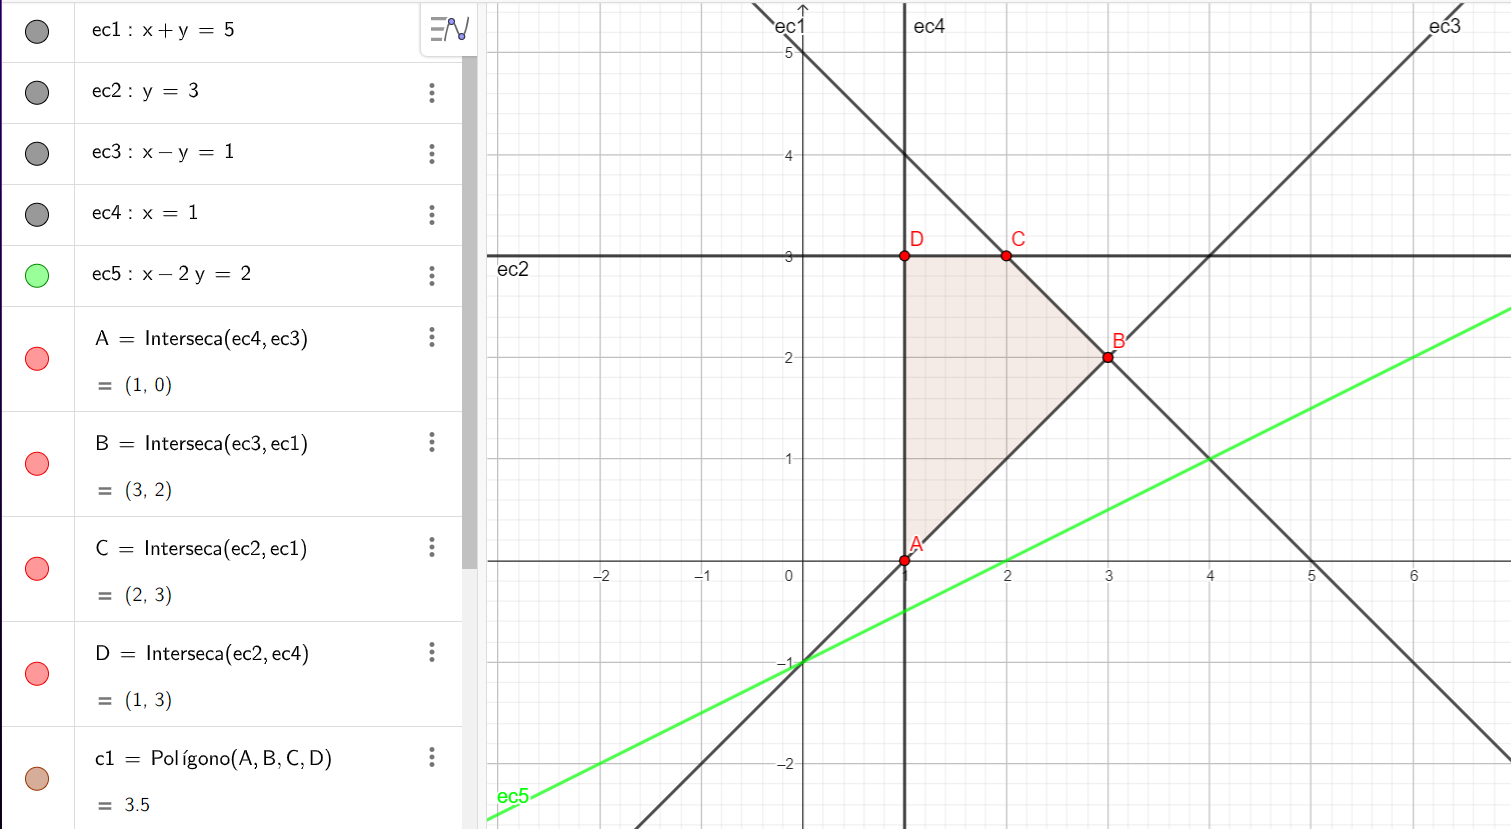
\includegraphics[width=0.6\textwidth]{img/Problema2Grafica.png}
\end{figure}
OBS:
\begin{itemize}
    \item La restriccion (5) de color verde es redundante.
    \item Lo de activo y no activo tengo que investigarlo mas o pedirle a alguien que me lo explique.
\end{itemize}
\begin{center}
    \begin{tabular}{|c|c|c|}
        \hline
        \textbf{Vertice ($x_1,x_2$)} & Z &  \\ \hline
        A(1, 0) & 2 & \\ \hline
        B(3, 2) & -6 & \\ \hline
        C(2, 3) & -14 & \\ \hline
        D(1, 3) & -16 & * \\ \hline
    \end{tabular}
\end{center}
\subsection{Algunas definiciones:}
\begin{itemize}
    \item \textbf{Solución factible:} todos los puntos $(x_1, x_2)$ deben satisfacer todas las restricciones.
    \item \textbf{Región factible:} conjunto de todas las soluciones factibles.
    \item \textbf{Vértices:} puntos de esquina o extremos de la región factible.
    \item \textbf{Optimo de un modelo lineal:} es un vértice de la región factible que maximiza o minimiza la función objetivo.
\end{itemize}

\newpage
\subsection*{Problema 3: Optimos Alternativos}
\subsubsection*{Función Objetivo:}
\begin{equation*}
    \begin{aligned}
        \text{Max} \quad & Z = 4x_1 + 3x_2 \\
        \text{s.a} \quad & 12x_1 + 9x_2 \leq 84 \quad &\textbf{Activa} \\
        & x_2 \leq 4 \quad &\textbf{Activa} \\
        & x_1, x_2 \geq 0
    \end{aligned}
\end{equation*}

\subsubsection*{Solución por método gráfico:}
\begin{figure}[H]
    \centering
    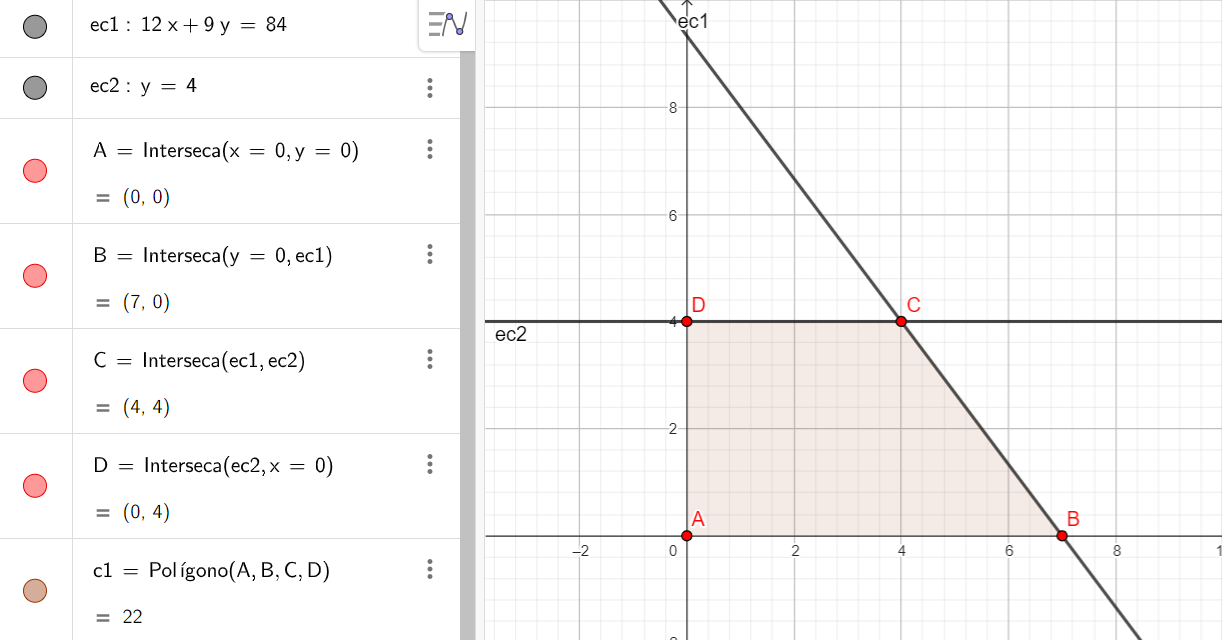
\includegraphics[width=1\textwidth]{img/Problema3Grafica.png}
\end{figure}
\begin{center}
    \begin{tabular}{|c|c|c|}
        \hline
        \textbf{Vertice ($x_1,x_2$)} & Z &  \\ \hline
        A(0, 0) & 0 & \\ \hline
        B(7, 0) & 28 & * \\ \hline
        C(4, 4) & 28 & * \\ \hline
        D(0, 4) & 12 & \\ \hline
    \end{tabular}
\end{center}
OBS:
\begin{itemize}
    \item Se puede observar que el vertice B y C son optimos alternativos.
\end{itemize}

\newpage
\subsection*{Problema 4: Variables sin restriccion de signo (S.R.S)}
\subsubsection*{Función Objetivo:}
\begin{equation*}
    \begin{aligned}
        \text{Max} \quad & Z = -3x_1 + 4x_2 \\
        \text{s.a} \quad & 5x_1 - 7x_2 \leq 35 \quad &\textbf{No Activa} \\
        & 2x_1 + 3x_2 \geq 6 \quad &\textbf{No Activa} \\
        & -2x_1 + 3x_2 \leq 12 \quad &\textbf{Activa} \\
        & 9x_1 + 13x_2 \leq 117 \quad &\textbf{No Activa} \\
        & x_1, x_2 \geq 0
    \end{aligned}
\end{equation*}

\subsubsection*{Solución por método gráfico:}
\begin{figure}[H]
    \centering
    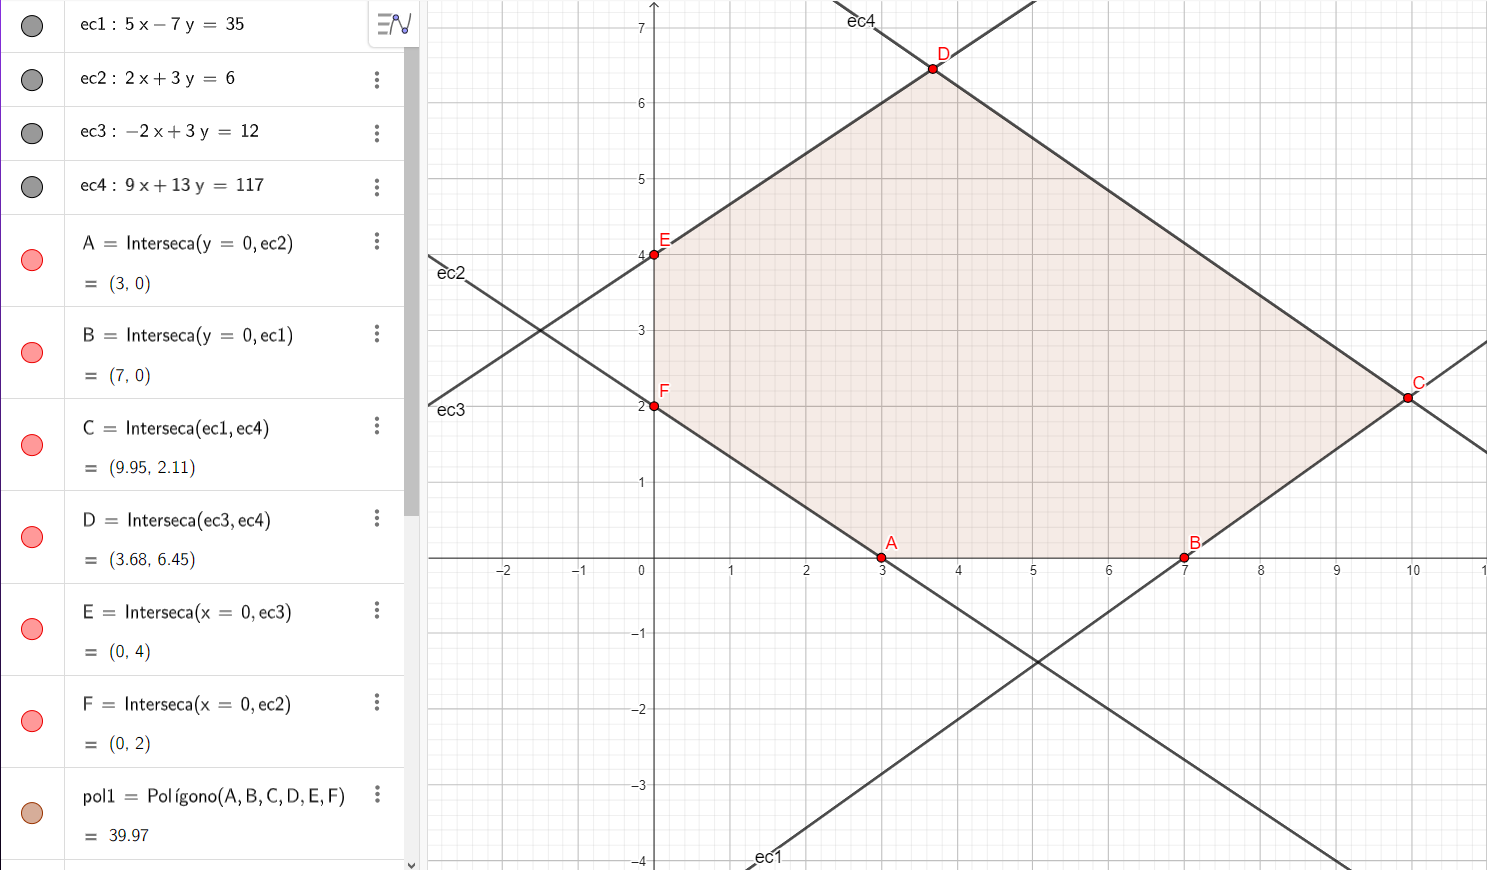
\includegraphics[width=1\textwidth]{img/Problema4Grafica.png}
\end{figure}

\begin{center}
    \begin{tabular}{|c|c|c|}
        \hline
        \textbf{Vertice ($x_1,x_2$)} & Z &  \\ \hline
        A(3, 0) & -9 & \\ \hline
        B(7, 0) & -21 & \\ \hline
        C(637/64, 120/67) & -22,695 & \\ \hline
        D(195/53, 342/53) & 14,774 & \\ \hline
        E(0, 4) & 16 & * \\ \hline
        F(0, 2) & 8 & \\ \hline
    \end{tabular}
\end{center}

\newpage
\subsection*{Problema 5: Región factible no acotada}
Un atleta debe tomar por lo menos 4 unidades de vitamina A, 6 unidades de vitamina B y 12 unidades de vitamina C cada día. Hay dos productos en polvo, P1 y P2, que por cada frasco, contienen las siguintes unidades de esas vitaminas:
\begin{center}
    \begin{tabular}{|c|c|c|c|}
        \hline
        & Vitamina A & Vitamina B & Vitamina C \\ \hline
        P1 & 4 & 1 & 4 \\ \hline
        P2 & 1 & 6 & 6 \\ \hline
    \end{tabular}
\end{center}

Si el precio de un frasco de P1 es de \$5000 y el de un frasco de P2 es de \$8000, se quiere averiguar cómo deben mezclarse ambos productos para obtener las vitaminas deseadas con el minimo precio. Formular Modelo y resolver por método gráfico.

\subsubsection*{Variables de Decisión:}
\begin{itemize}
    \item $x_1$: Cantidad de frascos de P1 a comprar.
    \item $x_2$: Cantidad de frascos de P2 a comprar.
\end{itemize}
\subsubsection*{Función Objetivo:}
\begin{equation*}
    \begin{aligned}
        \text{Max} \quad & Z = 5000x_1 + 8000x_2 \\
        \text{s.a} \quad & 4x_1 + x_2 \geq 4 \quad &\textbf{No Activa} \\
        & x_1 + 6x_2 \geq 6 \quad &\textbf{Activa} \\
        & 4x_1 + 6x_2 \geq 12 \quad &\textbf{Activa} \\
        & x_1, x_2 \geq 0
    \end{aligned}
\end{equation*}

\subsubsection*{Solución por método gráfico:}
\begin{figure}[H]
    \centering
    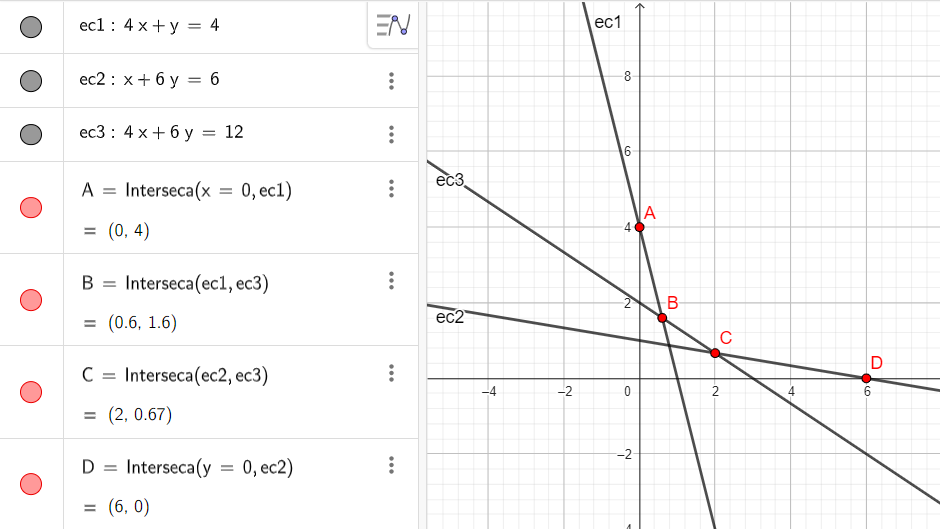
\includegraphics[width=0.5\textwidth]{img/Problema5Grafica.png}
\end{figure}

\begin{center}
    \begin{tabular}{|c|c|c|}
        \hline
        \textbf{Vertice ($x_1,x_2$)} & Z &  \\ \hline
        A(0, 4) & 32000 & \\ \hline
        B(3/5, 8/5) & 15800 & \\ \hline
        C(2, 2/3) & 15333 & * \\ \hline
        D(6, 0) & 30000 & \\ \hline
    \end{tabular}
\end{center}

\subsection*{Problema 6: Formulación con más de 2 variables de decisión}
La empresa MADERAS C.A es un fabricante de muebles. Hace tres estilos diferentes de mesas, A,B y C. Cada modelo de mesa requiere de una cierta cantidad de tiempo para el corte de las piezas, su montaje y pintura. MADERAS C.A, puede vender todas las unidades que fabrica. Es más, el modelo B se puede vender sin pintar. Utilizando los datos indicados, obtener el modelo lineal que permita determinar la máxima utilidad mensual que puede obtener la Empresa.

\begin{center}
    \begin{tabular}{|l|c|c|c|c|}
        \hline
        Modelo & Utilidad por mesa & Corte & Ensamblado & Pintura \\ \hline
        A & 17500 & 1 & 2 & 4 \\ \hline
        B & 20000 & 2 & 4 & 4 \\ \hline
        B sin pintar & 10000 & 2 & 4 & 0 \\ \hline
        C & 25000 & 3 & 7 & 5 \\ \hline
         & Disponibilidad mensual de HH & 200 & 298 & 148 \\ \hline
    \end{tabular}
\end{center}

\subsubsection*{Variables de Decisión:}
\begin{itemize}
    \item $x_1$: Cantidad de mesas A a fabricar.
    \item $x_2$: Cantidad de mesas B a fabricar.
    \item $x_3$: Cantidad de mesas B sin pintar a fabricar.
    \item $x_4$: Cantidad de mesas C a fabricar.
\end{itemize}

\subsubsection*{Función Objetivo:}
\begin{equation*}
    \begin{aligned}
        \text{Max} \quad & Z = 17500x_1 + 20000x_2 + 10000x_3 + 25000x_4 \\
        \text{s.a} \quad & x_1 + 2x_2 + 2x_3 + 3x_4 \leq 200 \\
        & 2x_1 + 4x_2 + 4x_3 + 7x_4 \leq 298 \\
        & 4x_1 + 4x_2 + 5x_4 \leq 148 \\
        & x_1, x_2, x_3, x_4 \geq 0
    \end{aligned}
\end{equation*}

OBS:
\begin{itemize}
    \item Cuando son más de 2 variables de decisión, el método gráfico no es la mejor opción, pues para calcular las intersecciones se vuelve caotico.
\end{itemize}

\subsection{Diagrama de flujo: Método Simplex}
\begin{center}
    \centering
    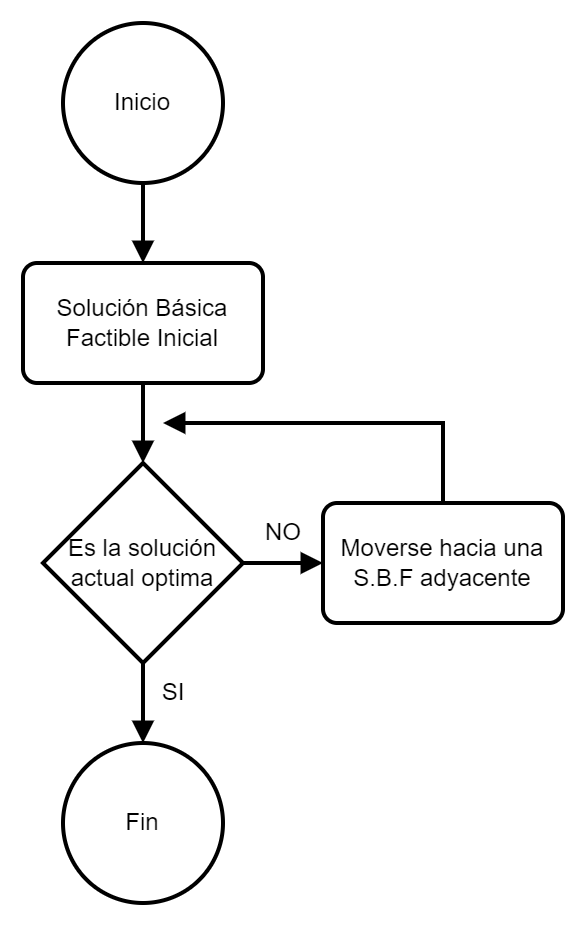
\includegraphics[width=0.4\textwidth]{diagram/Fig2.png}
\end{center}

\subsubsection*{Un poco de Teoría}
\begin{itemize}
    \item \textbf{Variables de holgura $s_i$}: Al introduccir variables de holgura cada restriccion se transforma en igualdad.
    \begin{itemize}
        \item \textbf{n}: cantidad de variables.
        \item \textbf{m}: cantidad de restricciones.
    \end{itemize}

    \item Un sistema con $n>m$ tiene infinitas soluciones.
    Para estos sistemas se define:
    \begin{itemize}
        \item Como $n-m$: cantidad de variables libres. Para encontrar soluciones al sistema se dan valores arbitrarios a las variables libres y se resuelve para el resto de variables.
        
        \item Si damos el valor cero a las variables obtenemos lo que llamaremos soluciones básicas.
        
        \item Si ademas los valores de las variables son mayor o igual a cero tenemos una solucion basica factible (S.B.F).
        
        OBS:
        \begin{itemize}
            \item S.B.F corresponde a un vertice de la región factible.
            \item Para un sistema $n \times m$ la cantidad de S.B.F es menor o igual a $\binom{n}{m} $.
            \item Dos vertices o S.B.F son adyacentes cuando tienen una arista de la R.F. en común.
        \end{itemize}
    \end{itemize}
\end{itemize}
\newpage
\subsection*{Problema 7: Método Simplex}
\subsubsection*{Función Objetivo:}
\begin{equation*}
    \begin{aligned}
        \text{Max} \quad & Z = 4x_1 + 3x_2 \\
        \text{s.a} \quad & 12x_1 + 14x_2 \leq 84 \quad & \textbf{Activa} \\
        & 3x_1 + 2x_2 \leq 18 \quad & \textbf{Activa} \\
        & x_2 \leq 4 \quad & \textbf{No Activa} \\
        & x_1, x_2 \geq 0
    \end{aligned}
\end{equation*}

\subsubsection*{Solución por método Simplex:}
\textbf{IMPORTANTE 'Pasos incompletos.'}

\textbf{Paso 1: Agregar variables de holgura y eliminar desigualdades.}
\begin{equation*}
    \begin{aligned}
        \text{Max} \quad & Z = 4x_1 + 3x_2 \\
        \text{s.a} \quad & 12x_1 + 14x_2 + s_1 = 84 \\
        & 3x_1 + 2x_2 + s_2 = 18 \\
        & x_2 + s_3 = 4\\
        & x_1, x_2, s_1, s_2, s_3 \geq 0
    \end{aligned}
\end{equation*}

\textbf{Paso 2: Crear tabla Simplex inicial.}
\begin{center}
    \begin{tabular}{|c|c|c|c|c|c|c|c|c|}
        \hline
        & & 4 & 3 & 0 & 0 & 0 &  &  \\ \hline
        $c_j$ & \textbf{V.B} & $x_1$ & $x_2$ & $s_1$ & $s_2$ & $s_3$ & RHS & $\displaystyle\frac{RHS}{coef_{ij^*}}$ \\ \hline
        0 & $s_1$ & 12 & 14 & 1 & 0 & 0 & 84 & 84/12 = 7 \\ \hline
        0 & $s_2$ & 3 & 2 & 0 & 1 & 0 & 18 & 18/3 = 6 \\ \hline
        0 & $s_3$ & 0 & 1 & 0 & 0 & 1 & 4 & 4/0 = - \\ \hline
        & $Z_j$ & 0 & 0 & 0 & 0 & 0 & \underline{0} &  \\ \hline
        & $c_j - Z_j$ & 4 & 3 & 0 & 0 & 0 &  &  \\ \hline
    \end{tabular}
\end{center}
OBS:
\begin{itemize}
    \item Para calcular $Z_j = c_j \times x_j $
    \begin{center}
        Ejemplo: $Z_{x_1} = c_1 \times x_1 + c_2 \times x_1 + c_3 \times x_1 = 0 \times 12 + 0 \times 3 + 0 \times 0 = 0$
    \end{center}

    \item Creo que deberia ser la columna $c_i$ y no $c_j$.
    \item De hecho $c_j$ deberia estar arriba de \textbf{V.B}.
\end{itemize}

\textbf{Paso 3: Buscamos la variable que entra.}
\begin{center}
    $V_{in} = \text{columna Max} \{c_j-Z_j\} = X_{j^*} \Rightarrow V_{in} = 4 = x_1$
\end{center}
OBS:
\begin{itemize}
    \item Como estamos máximizando la función objetivo, buscamos el valor más grande en la fila de $c_j - Z_j$.
\end{itemize}

\textbf{Paso 4: Buscamos la variable que sale.}
\begin{center}
    $V_{out} = \text{Min} \left\{ \frac{RHS}{coef_{ij^*}} \right\} = i^* \Rightarrow V_{out} = 6 = s_2$
\end{center}
OBS:
\begin{itemize}
    \item Como estamos máximizando la función objetivo, buscamos el valor más pequeño en la columna de $\displaystyle\frac{RHS}{coef_{ij^*}}$, pues es la holgura que es menos influyente.
\end{itemize}

\textbf{Paso 5: Calculamos el pivote.}
\begin{center}
    $\text{Pivote} = a_{i^*j^*} = a_{21} = 3$
\end{center}

\textbf{Paso 6: Creamos una ecuación pivote.}
\begin{equation*}
    \textbf{N.E.P} = \frac{\textbf{E.P.A}}{P} \\
    \Rightarrow \frac{\begin{array}{cccccc} 3 & 2 & 0 & 1 & 0 & 18\end{array}}{3} = \begin{array}{cccccc} 1 & \frac{2}{3} & 0 & \frac{1}{3} & 0 & 6\end{array}
\end{equation*}
OBS:
\begin{itemize}
    \item \textbf{N.E.P}: Nueva Ecuación Pivote (como entra $x_1$ en la tabla se escribe esta ecuación).
    \item \textbf{E.P.A}: Ecuación Pivote Actual (como sale $s_2$ ocupamos esa ecuación).
    \item $P = Pivote$
\end{itemize}

\textbf{Paso 7: Actualizamos las ecuación que se quedan.}
\begin{equation*}
    \begin{array}{ccccccc}
        s_1: & 12 & 14 & 1 & 0 & 0 & 84 \\
        -(12) & 1 & 2/3 & 0 & 1/3 & 0 & 6 \\
        \\ \hline \\
        & 0 & 6 & 1 & -4 & 0 & 12 
    \end{array}
\end{equation*}
\\
\begin{equation*}
    \begin{array}{ccccccc}
        s_3: & 0 & 1 & 0 & 0 & 1 & 4 \\
        -(0) & 1 & 2/3 & 0 & 1/3 & 0 & 6 \\
        \\ \hline \\
        & 0 & 1 & 0 & 0 & 1 & 4 
    \end{array}
\end{equation*}

\textbf{Paso 8: Actualizamos la tabla simplex con las nuevas ecuaciones.}
\begin{center}
    \begin{tabular}{|c|c|c|c|c|c|c|c|c|}
        \hline
        & & 4 & 3 & 0 & 0 & 0 &  &  \\ \hline
        $c_j$ & \textbf{V.B} & $x_1$ & $x_2$ & $s_1$ & $s_2$ & $s_3$ & RHS & $\displaystyle\frac{RHS}{coef_{ij^*}}$ \\ \hline
        0 & $s_1$ & 0 & 6 & 1 & -4 & 0 & 12 & 12/6 = 2\\ \hline
        4 & $x_1$ & 1 & 2/3 & 0 & 1/3 & 0 & 6 & 6/(2/3) = 9\\ \hline
        0 & $s_3$ & 0 & 1 & 0 & 0 & 1 & 4 & 4/1 = 4\\ \hline
        & $Z_j$ & 4 & 8/3 & 0 & 4/3 & 0 & \underline{24} &  \\ \hline
        & $c_j - Z_j$ & 0 & 1/3 & 0 & -4/3 & 0 &  &  \\ \hline
    \end{tabular}
\end{center}

\textbf{Paso 9: Utilizamos el criterio de optimalidad.}
\begin{center}
    $c_j - Z_j \leq 0 \quad \forall j$
\end{center}

Como $c_j - Z_j$ no es menor o igual a 0, entonces repetimos el ciclo desde el paso 3.

\textbf{Paso 10: Buscamos la variable que entra.}
\begin{center}
    $V_{in} = \text{columna Max} \{c_j-Z_j\} = X_{j^*} \Rightarrow V_{in} = 3= x_2$
\end{center}

\textbf{Paso 11: Buscamos la variable que sale.}
\begin{center}
    $V_{out} = \text{Min} \left\{ \frac{RHS}{coef_{ij^*}} \right\} = i^* \Rightarrow V_{out} = 2 = s_1$
\end{center}

\textbf{Paso 12: Calculamos el pivote.}
\begin{center}
    $\text{Pivote} = a_{i^*j^*} = a_{12} = 6$
\end{center}

\textbf{Paso 13: Creamos una ecuación pivote.}
\begin{equation*}
    \textbf{N.E.P} = \frac{\textbf{E.P.A}}{P} \\
    \Rightarrow \frac{\begin{array}{cccccc} 0 & 6 & 1 & -4 & 0 & 12 \end{array}}{6} = \begin{array}{cccccc} 0 & 1 & 1/6 & -2/3 & 0 & 2 \end{array}
\end{equation*}

\textbf{Paso 14: Actualizamos las ecuación que se quedan.}
\begin{equation*}
    \begin{array}{ccccccc}
        x_1: & 1 & 2/3 & 0 & 1/3 & 0 & 6 \\
        -(2/3) & 0 & 1 & 1/6 & -2/3 & 0 & 2 \\
        \\ \hline \\
        & 1 & 0 & -1/9 & 7/9 & 0 & 14/3 
    \end{array}
\end{equation*}
\\
\begin{equation*}
    \begin{array}{ccccccc}
        s_3: & 0 & 1 & 0 & 0 & 1 & 4 \\
        -(1) & 0 & 1 & 1/6 & -2/3 & 0 & 2 \\
        \\ \hline \\
        & 0 & 0 & -1/6 & 2/3 & 1 & 2
    \end{array}
\end{equation*}

\textbf{Paso 15: Actualizamos la tabla simplex con las nuevas ecuaciones.}
\begin{center}
    \begin{tabular}{|c|c|c|c|c|c|c|c|c|}
        \hline
        & & 4 & 3 & 0 & 0 & 0 &  &  \\ \hline
        $c_j$ & \textbf{V.B} & $x_1$ & $x_2$ & $s_1$ & $s_2$ & $s_3$ & RHS & $\displaystyle\frac{RHS}{coef_{ij^*}}$ \\ \hline
        3 & $x_2$ & 0 & 1 & 1/6 & -2/3 & 0 & 2 & \\ \hline
        4 & $x_1$ & 1 & 0 & -1/9 & 7/9 & 0 & 14/3 & \\ \hline
        0 & $s_3$ & 0 & 0 & -1/6 & 2/3 & 1 & 2 & \\ \hline
        & $Z_j$ & 4 & 3 & 1/18 & 10/9 & 0 & \underline{74/3} &  \\ \hline
        & $c_j - Z_j$ & 0 & 0 & -1/18 & -10/9 & 0 &  &  \\ \hline
    \end{tabular}
\end{center}

\newpage
\textbf{Paso 16: Utilizamos el criterio de optimalidad.}
\begin{center}
    $c_j - Z_j \leq 0 \quad \forall j$
\end{center}

Como $c_j - Z_j$ es menor o igual a 0, entonces hemos llegado a la solución óptima.
\textbf{Solución:}
\begin{align*}
    x_1 &= 14/3 \\
    x_2 &= 2 \\
    s_1 &= 0 \qquad \textbf{Recurso escaso} \Rightarrow \textbf{Restricción Activa}\\
    s_2 &= 0 \qquad \textbf{Recurso escaso} \Rightarrow \textbf{Restricción Activa}\\
    s_3 &= 2 \qquad \textbf{Recurso abundante} \Rightarrow \textbf{Restricción No Activa}\\
    Z &= 74/3
\end{align*}

\subsection*{Solución por método gráfico}
\begin{figure}[H]
    \centering
    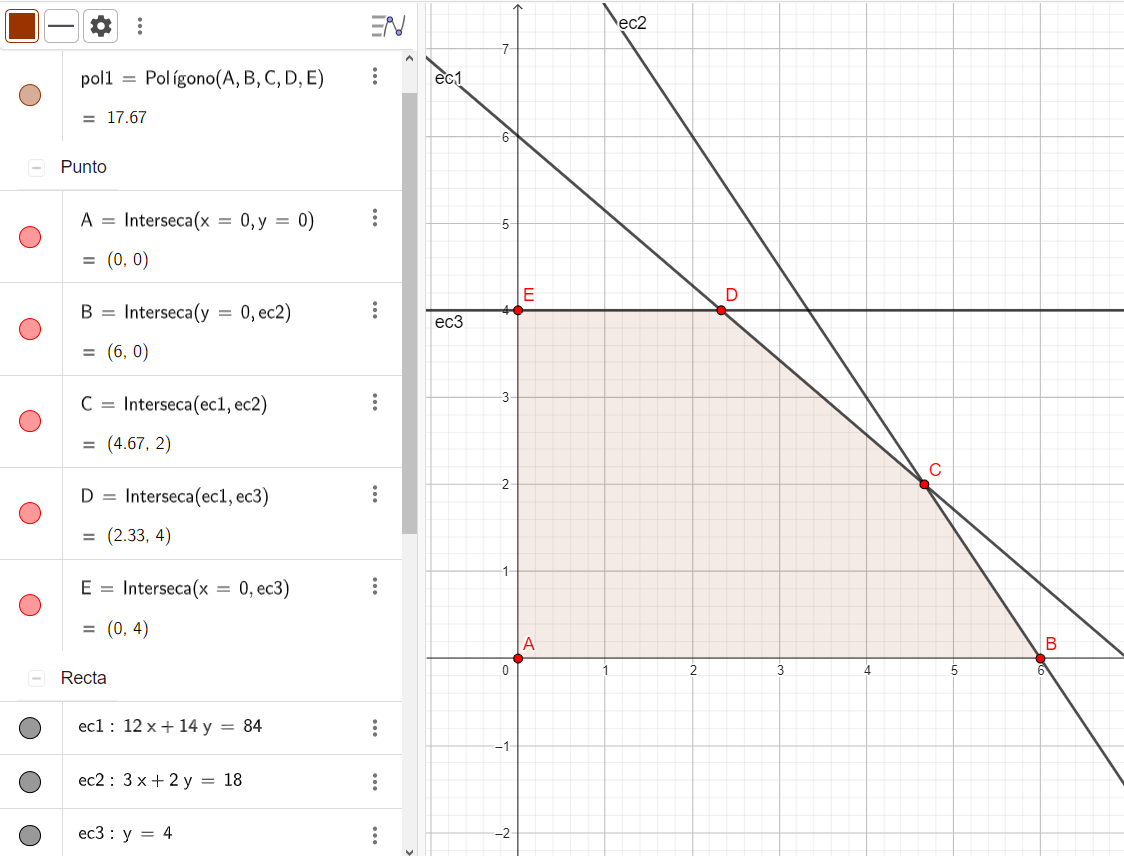
\includegraphics[width=0.9\textwidth]{img/Problema7Grafica.png}
\end{figure}

\begin{center}
    \begin{tabular}{|c|c|c|}
        \hline
        \textbf{Vertice ($x_1,x_2$)} & Z &  \\ \hline
        A(0, 0) & 0 & \\ \hline
        B(6, 0) & 24 & \\ \hline
        C(14/3, 2) & 74/3 & * \\ \hline
        D(7/3, 4) & 64/3 & \\ \hline
        E(0, 4) & 12 & \\ \hline
    \end{tabular}
\end{center}

Por lo tanto, queda demostrado que el método Simplex y el método gráfico nos entregan el valor optimo.
\newpage

\subsection*{Problema 8: Configuración de tabla Simplex}
\subsubsection*{Función Objetivo:}
\begin{equation*}
    \begin{aligned}
        \text{Max} \quad & Z = 5x_1 + 4x_2\\
        \text{s.a} \quad & 6x_1 + 4x_2 \leq 24 \\
        & x_1 + 2x_2 \leq 6 \\
        & -x_1 + x_2 \leq 1 \\
        & x_2 \leq 2 \\
        & x_1, x_2 \geq 0
    \end{aligned}
\end{equation*}

\subsubsection*{Solución por método Simplex:}
\noindent
\textbf{Paso 1: Si el problema es un problema de minimización, multiplica la función objetivo por -1.}
\\
\textbf{Paso 2: Si la formulación del problema contiene algunas restricciones con lados derechos negativos, multiplique cada restricción por -1.}
\\
\textbf{Paso 3: Agregue una variable de holgura $S_i$ a cada restricción $\leq$.}
\begin{equation*}
    \begin{aligned}
        & 6x_1 + 4x_2 + s_1 \leq 24 \\
        & x_1 + 2x_2 + s_2 \leq 6 \\
        & -x_1 + x_2 + s_3 \leq 1 \\
        & x_2 + s_4 \leq 2 \\
        & x_1, x_2, s_1, s_2, s_3, s_4 \geq 0
    \end{aligned}
\end{equation*}
\textbf{Paso 4: Reste una variable de exceso $R_i$ y sume una variable artificial para cada $\geq$ restricción.}
\\
\textbf{Paso 5: Agregue una variable artificial a cada restricción =.}
\\
\textbf{Paso 6: Establecer cada variable de holgura y excedente con coeficiente igual a cero en la función objetivo.}
\begin{equation*}
    \begin{aligned}
        & 6x_1 + 4x_2 + s_1 = 24 \\
        & x_1 + 2x_2 + s_2 = 6 \\
        & -x_1 + x_2 + s_3 = 1 \\
        & x_2 + s_4 = 2 \\
        & x_1, x_2, s_1, s_2, s_3, s_4 \geq 0
    \end{aligned}
\end{equation*}
\textbf{Paso 7: Establecer el coeficiente de cada variable artificial en la función objetivo igual a -M, donde M es una número muy grande.}
\\
\textbf{Paso 8: Cada variable de holgura y  artificial se convierte en una de las variables básicas en el cálculo solución básica factible inicial.}

\newpage
\noindent
\textbf{Paso 9: Escribir la tabla simplex inicial.}
\begin{center}
    \begin{tabular}{|c|c|c|c|c|c|c|c|c|}
        \hline
        $C_j$ & & 5 & 4 & 0 & 0 & 0 & 0 & \\ \hline
        & \textbf{V.B} & $x_1$ & $x_2$ & $s_1$ & $s_2$ & $s_3$ & $s_4$ & RHS \\ \hline
        0 & $s_1$ & 6 & 4 & 1 & 0 & 0 & 0 & 24 \\ \hline
        0 & $s_2$ & 1 & 2 & 0 & 1 & 0 & 0 & 6 \\ \hline
        0 & $s_3$ & -1 & 1 & 0 & 0 & 1 & 0 & 1 \\ \hline
        0 & $s_4$ & 0 & 1 & 0 & 0 & 0 & 1 & 2 \\ \hline
    \end{tabular}
\end{center}
\textbf{Paso 10: Calcular la fila $Z_j$ para la nueva Tabla.}
\\
OBS:
\begin{itemize}
    \item Para cada columna j, multiplica los coeficientes en la función objetivo de las variables básicas por los números correspondientes en la columna j y sumarlos
\end{itemize}
\begin{center}
    \begin{tabular}{|c|c|c|c|c|c|c|c|c|}
        \hline
        $C_j$ & & 5 & 4 & 0 & 0 & 0 & 0 & \\ \hline
        & \textbf{V.B} & $x_1$ & $x_2$ & $s_1$ & $s_2$ & $s_3$ & $s_4$ & RHS \\ \hline
        \cellcolor{green!50}0 & $s_1$ & \cellcolor{green!50}6 & 4 & 1 & 0 & 0 & 0 & 24 \\ \hline
        \cellcolor{blue!50}0 & $s_2$ & \cellcolor{blue!50}1 & 2 & 0 & 1 & 0 & 0 & 6 \\ \hline
        \cellcolor{orange!50}0 & $s_3$ & \cellcolor{orange!50}-1 & 1 & 0 & 0 & 1 & 0 & 1 \\ \hline
        \cellcolor{yellow!50}0 & $s_4$ & \cellcolor{yellow!50}0 & 1 & 0 & 0 & 0 & 1 & 2 \\ \hline
        & $Z_j$ & \cellcolor{red!50}0 & 0 & 0 & 0 & 0 & 0 & \underline{0} \\ \hline
        & $C_j - Z_j$ & & & & & & & \\ \hline
    \end{tabular}
\end{center}
\begin{equation*}
    \colorbox{green!50}{0} \times \colorbox{green!50}{6} + \colorbox{blue!50}{0} \times \colorbox{blue!50}{1} + \colorbox{orange!50}{0} \times \colorbox{orange!50}{(-1)} + \colorbox{yellow!50}{0} \times \colorbox{yellow!50}{0} = \colorbox{red!50}{0}
\end{equation*}
\textbf{Paso 11: : Calcular la fila $C_j - Z_j$ para nueva tabla.}
\\
Para cada columna j, reste la fila $C_j$ de la fila $Z_j$.:
\begin{itemize}
    \item Si ninguno de los valores en la fila $C_j - Z_j$ es positivo,  FIN. 
    Redactar la solución óptima.
    \item Si el valor $C_j - Z_j$ de alguna variable no básica es 0,  existen soluciones óptimas alternativas.
    \item Si existe una variable artificial en la base con un valor positivo, el problema es inviable. 
\end{itemize}
\begin{center}
    \begin{tabular}{|c|c|c|c|c|c|c|c|c|}
        \hline
        $C_j$ & & \cellcolor{green!50}5 & 4 & 0 & 0 & 0 & 0 & \\ \hline
        & \textbf{V.B} & $x_1$ & $x_2$ & $s_1$ & $s_2$ & $s_3$ & $s_4$ & RHS \\ \hline
        0 & $s_1$ & 6 & 4 & 1 & 0 & 0 & 0 & 24 \\ \hline
        0 & $s_2$ & 1 & 2 & 0 & 1 & 0 & 0 & 6 \\ \hline
        0 & $s_3$ & -1 & 1 & 0 & 0 & 1 & 0 & 1 \\ \hline
        0 & $s_4$ & 0 & 1 & 0 & 0 & 0 & 1 & 2 \\ \hline
        & $Z_j$ & \cellcolor{red!50}0 & 0 & 0 & 0 & 0 & 0 & \underline{0} \\ \hline
        & $C_j - Z_j$ & \cellcolor{orange!50}5 & 4 & 0 & 0 & 0 & 0 & \\ \hline
    \end{tabular}
\end{center}
\begin{equation*}
    \colorbox{green!50}{5} - \colorbox{red!50}{0} = \colorbox{orange!50}{5}
\end{equation*}

\newpage
\textbf{Paso 12: Determinar la variable entrante identificando la variable con el valor más positivo en la fila $C_j - Z_j$ (La columna de entrada se llama la columna pivote)}
\begin{center}
    \begin{equation*}
        \colorbox{green!50}{$V_{in}$} = \text{columna Max} \{C_j-Z_j\} = X_{j^*} \Rightarrow V_{in} = x_1 : 5
    \end{equation*}
\end{center}
OBS:
\begin{itemize}
    \item Como estamos máximizando la función objetivo, buscamos el valor más grande en la fila de $C_j - Z_j$.
\end{itemize}

\textbf{Paso 13: Determinar la variable saliente.}
\begin{itemize}
    \item Por cada número positivo en la columna de entrada, calcular la relación de los valores del lado derecho dividido por estos valores de columna entrantes.
    \item Si no hay valores positivos en la entrada columna, DETENER; el problema es ilimitado.
    \item En caso contrario, seleccione la variable con el mínimo relación.(La fila saliente se llama fila pivote).
\end{itemize}
\begin{center}
    \begin{tabular}{|c|c|c|c|c|c|c|c|c|}
        \hline
        $C_j$ & & 5 & 4 & 0 & 0 & 0 & 0 & \\ \hline
        & \textbf{V.B} & $x_1$ & $x_2$ & $s_1$ & $s_2$ & $s_3$ & $s_4$ & RHS \\ \hline
        0 & $s_1$ & \cellcolor{orange!50}6 & 4 & 1 & 0 & 0 & 0 & \cellcolor{yellow!50}24 \\ \hline
        0 & $s_2$ & 1 & 2 & 0 & 1 & 0 & 0 & 6 \\ \hline
        0 & $s_3$ & -1 & 1 & 0 & 0 & 1 & 0 & 1 \\ \hline
        0 & $s_4$ & 0 & 1 & 0 & 0 & 0 & 1 & 2 \\ \hline
        & $Z_j$ & 0 & 0 & 0 & 0 & 0 & 0 & \underline{0} \\ \hline
        & $C_j - Z_j$ & 5 & 4 & 0 & 0 & 0 & 0 & \\ \hline
    \end{tabular}
\end{center}
\begin{align*}
    s_1: \frac{\colorbox{yellow!50}{24}}{\colorbox{orange!50}6} = 4 \qquad & s_2: \frac{6}{1} = 6 \qquad & s_3: \frac{1}{-1} = \text{-} \qquad & s_4: \frac{2}{0} = \text{-}
\end{align*}
\begin{center}
    \begin{equation*}
        \colorbox{red!50}{$V_{out}$} = \text{Min} \left\{ \frac{RHS}{coef_{ij^*}} \right\} = i^* \Rightarrow V_{out} = s_1 : 4
    \end{equation*}
\end{center}

\begin{center}
    \begin{tabular}{|c|c|g|c|c|c|c|c|c|}
        \hline
        $C_j$ & & 5 & 4 & 0 & 0 & 0 & 0 & \\ \hline
        & \textbf{V.B} & $x_1$ & $x_2$ & $s_1$ & $s_2$ & $s_3$ & $s_4$ & RHS \\ \hline
        \rowcolor{red!50}0 & $s_1$ & 6 & 4 & 1 & 0 & 0 & 0 & 24 \\ \hline
        0 & $s_2$ & 1 & 2 & 0 & 1 & 0 & 0 & 6 \\ \hline
        0 & $s_3$ & -1 & 1 & 0 & 0 & 1 & 0 & 1 \\ \hline
        0 & $s_4$ & 0 & 1 & 0 & 0 & 0 & 1 & 2 \\ \hline
        & $Z_j$ & 0 & 0 & 0 & 0 & 0 & 0 & \underline{0} \\ \hline
        & $C_j - Z_j$ & 5 & 4 & 0 & 0 & 0 & 0 & \\ \hline
    \end{tabular}
\end{center}
\begin{center}
    $\text{Pivote} = a_{i^*j^*} = a_{11} = 6$
\end{center}

\newpage
\textbf{Paso 14: Generar la siguiente tabla.}

\begin{itemize}
    \item Divida la fila de pivote por el elemento de pivote (el entrada en la intersección de la fila de pivote y el pivote columna) para obtener una nueva fila. Denotamos esta nueva fila (*)
    \begin{center}
        \begin{equation*}
            \textbf{N.E.P} = \frac{\textbf{E.P.A}}{P} \Rightarrow \frac{\begin{array}{ccccccc} 6 & 4 & 1 & 0 & 0 & 0 & 24\end{array}}{6} = \begin{array}{ccccccc} 1 & \frac{2}{3} & \frac{1}{6} & 0 & 0 & 0 & 4 \end{array}
        \end{equation*}
    \end{center}
        OBS:
        \begin{itemize}
            \item \textbf{N.E.P}: Nueva Ecuación Pivote (como entra $x_1$ en la tabla se escribe esta ecuación).
            \item \textbf{E.P.A}: Ecuación Pivote Actual (como sale $s_1$ ocupamos esa ecuación).
            \item $P = Pivote$
        \end{itemize}
    \item Reemplace cada fila i que no sea pivote con: [nueva fila i] = [fila actual i] - [($a_{ij}$) x (fila (*))], donde  $a_{ij}$ es el valor al ingresar la columna j de la fila i.
    \begin{equation*}
        \begin{array}{cccccccc}
            s_2: & 1 & 2 & 0 & 1 & 0 & 0 & 6 \\
            -(1) & 1 & 2/3 & 1/6 & 0 & 0 & 0 & 4 \\
            \\ \hline \\
            & 0 & 4/3 & -1/6 & 1 & 0 & 0 & 2
        \end{array}
    \end{equation*}
    \\
    \begin{equation*}
        \begin{array}{cccccccc}
            s_3: & -1 & 1 & 0 & 0 & 1 & 0 & 1 \\
            -(-1) & 1 & 2/3 & 1/6 & 0 & 0 & 0 & 4 \\
            \\ \hline \\
            & 0 & 5/3 & 1/6 & 0 & 1 & 0 & 5
        \end{array}
    \end{equation*}
    \\
    \begin{equation*}
        \begin{array}{cccccccc}
            s_4: & 0 & 1 & 0 & 0 & 0 & 1 & 2 \\
            -(0) & 1 & 2/3 & 1/6 & 0 & 0 & 0 & 4 \\
            \\ \hline \\
            & 0 & 1 & 0 & 0 & 0 & 1 & 2
        \end{array}
    \end{equation*}
\end{itemize}
\begin{center}
    \begin{tabular}{|c|c|c|c|c|c|c|c|c|}
        \hline
        $C_j$ & & 5 & 4 & 0 & 0 & 0 & 0 & \\ \hline
        & \textbf{V.B} & $x_1$ & $x_2$ & $s_1$ & $s_2$ & $s_3$ & $s_4$ & RHS \\ \hline
        5 & $x_1$ & 1 & 2/3 & 1/6 & 0 & 0 & 0 & 4 \\ \hline
        0 & $s_2$ & 0 & 4/3 & -1/6 & 1 & 0 & 0 & 2 \\ \hline
        0 & $s_3$ & 0 & 5/3 & 1/6 & 0 & 1 & 0 & 5 \\ \hline
        0 & $s_4$ & 0 & 1 & 0 & 0 & 0 & 1 & 2 \\ \hline
        & $Z_j$ & 5 & 5/3 & 5/6 & 0 & 0 & 0 & \underline{20} \\ \hline
        & $C_j - Z_j$ & 0 & 7/3 & -5/3 & 0 & 0 & 0 & \\ \hline
    \end{tabular}
\end{center}
\newpage
\textbf{Paso 15: Ir a Paso 10.}
\begin{center}
    \begin{equation*}
        \colorbox{green!50}{$V_{in}$} = \text{columna Max} \{C_j-Z_j\} = X_{j^*} \Rightarrow V_{in} = x_2 : \frac{7}{3} 
    \end{equation*}
\end{center}
\begin{align*}
    x_1: \frac{4}{\frac{2}{3}} = 6 \qquad & s_2: \frac{2}{\frac{4}{3}} = \frac{3}{2} \qquad & s_3: \frac{5}{\frac{5}{3}} = 3 \qquad & s_4: \frac{2}{1} = 2
\end{align*}
\begin{center}
    \begin{equation*}
        \colorbox{red!50}{$V_{out}$} = \text{Min} \left\{ \frac{RHS}{coef_{ij^*}} \right\} = i^* \Rightarrow V_{out} = s_2 : \frac{3}{2}
    \end{equation*}
\end{center}
\begin{equation*}
    \begin{aligned}
        \text{Pivote} = a_{i^*j^*} = a_{22} = 4/3
    \end{aligned}
\end{equation*}
\begin{center}
    \begin{tabular}{|c|c|c|g|c|c|c|c|c|}
        \hline
        $C_j$ & & 5 & 4 & 0 & 0 & 0 & 0 & \\ \hline
        & \textbf{V.B} & $x_1$ & $x_2$ & $s_1$ & $s_2$ & $s_3$ & $s_4$ & RHS \\ \hline
        5 & $x_1$ & 1 & 2/3 & 1/6 & 0 & 0 & 0 & 4 \\ \hline
        \rowcolor{red!50}0 & $s_2$ & 0 & 4/3 & -1/6 & 1 & 0 & 0 & 2 \\ \hline
        0 & $s_3$ & 0 & 5/3 & 1/6 & 0 & 1 & 0 & 5 \\ \hline
        0 & $s_4$ & 0 & 1 & 0 & 0 & 0 & 1 & 2 \\ \hline
        & $Z_j$ & 5 & 5/3 & 5/6 & 0 & 0 & 0 & \underline{20} \\ \hline
        & $C_j - Z_j$ & 0 & 7/3 & -5/3 & 0 & 0 & 0 & \\ \hline
    \end{tabular}
\end{center}
\begin{center}
    \begin{equation*}
        \textbf{N.E.P} = \frac{\textbf{E.P.A}}{P} \Rightarrow \frac{\begin{array}{ccccccc} 0 & 4/3 & -1/6 & 1 & 0 & 0 & 2\end{array}}{4/3} = \begin{array}{ccccccc} 0 & 1 & \frac{-1}{8} & \frac{3}{4} & 0 & 0 & \frac{3}{2} \end{array}
    \end{equation*}
\end{center}
\begin{equation*}
    \begin{array}{cccccccc}
        x_1: & 1 & 2/3 & 1/6 & 0 & 0 & 0 & 4 \\
        -(2/3) & 0 & 1 & -1/8 & 3/4 & 0 & 0 & 3/2 \\
        \\ \hline \\
        & 1 & 0 & 1/4 & -1/2 & 0 & 0 & 3
    \end{array}
\end{equation*}
\\
\begin{equation*}
    \begin{array}{cccccccc}
        s_3: & 0 & 5/3 & 1/6 & 0 & 1 & 0 & 5 \\
        -(5/3) & 0 & 1 & -1/8 & 3/4 & 0 & 0 & 3/2 \\
        \\ \hline \\
        & 0 & 0 & 3/8 & -5/4 & 1 & 0 & 5/2
    \end{array}
\end{equation*}
\\
\begin{equation*}
    \begin{array}{cccccccc}
        s_4: & 0 & 1 & 0 & 0 & 0 & 1 & 2 \\
        -(1) & 0 & 1 & -1/8 & 3/4 & 0 & 0 & 3/2 \\
        \\ \hline \\
        & 0 & 0 & 1/8 & -3/4 & 0 & 1 & 1/2
    \end{array}
\end{equation*}
\begin{center}
    \begin{tabular}{|c|c|c|c|c|c|c|c|c|}
        \hline
        $C_j$ & & 5 & 4 & 0 & 0 & 0 & 0 & \\ \hline
        & \textbf{V.B} & $x_1$ & $x_2$ & $s_1$ & $s_2$ & $s_3$ & $s_4$ & RHS \\ \hline
        5 & $x_1$ & 1 & 0 & 1/4 & -1/2 & 0 & 0 & 3 \\ \hline
        4 & $x_2$ & 0 & 1 & -1/8 & 3/4 & 0 & 0 & 3/2 \\ \hline
        0 & $s_3$ & 0 & 0 & 3/8 & -5/4 & 1 & 0 & 5/2 \\ \hline
        0 & $s_4$ & 0 & 0 & 1/8 & -3/4 & 0 & 1 & 1/2 \\ \hline
        & $Z_j$ & 5 & 4 & 3/4 & 1/2 & 0 & 0 & \underline{21} \\ \hline
        & $C_j - Z_j$ & 0 & 0 & -3/4 & -1/2 & 0 & 0 & \\ \hline
    \end{tabular}
\end{center}
\textbf{Paso R11: Calcular la fila $C_j - Z_j$ para nueva tabla.}
\begin{itemize}
    \item Si ninguno de los valores en la fila $C_j - Z_j$ es positivo,  FIN.
\end{itemize}
\begin{center}
    $c_j - Z_j \leq 0 \quad \forall j$
\end{center}

Como $c_j - Z_j$ es menor o igual a 0, entonces hemos llegado a la solución óptima.
\textbf{Solución:}
\begin{align*}
    x_1 &= 3 \\
    x_2 &= \displaystyle\frac{3}{2} \\
    s_1 &= 0 \qquad \textbf{Recurso escaso} \Rightarrow \textbf{Restricción Activa}\\
    s_2 &= 0 \qquad \textbf{Recurso escaso} \Rightarrow \textbf{Restricción Activa}\\
    s_3 &= \displaystyle\frac{5}{2} \qquad \textbf{Recurso abundante} \Rightarrow \textbf{Restricción No Activa}\\
    s_4 &= \displaystyle\frac{1}{2} \qquad \textbf{Recurso abundante} \Rightarrow \textbf{Restricción No Activa}\\
    Z &= 21
\end{align*}

\newpage
\subsection*{Problema 9: Configuración de tabla Simplex y Metodo M}

\subsubsection*{Función Objetivo:}
\begin{equation*}
    \begin{aligned}
        \text{Min} \quad & Z = 2x_1 - 3x_2 - 4x_3\\
        \text{s.a} \quad & x_1 + x_2 + x_3 \leq 30 \\
        & 2x_1 + x_2 + x_3 \geq 60 \\
        & x_1 - x_2 + 2x_3 = 20 \\
        & x_1, x_2, x_3 \geq 0
    \end{aligned}
\end{equation*}

\subsubsection*{Solución por método Simplex:}
\noindent
\textbf{Paso 1: Si el problema es un problema de minimización, multiplica la función objetivo por -1.}
\begin{equation*}
    Max \quad -Z = -2x_1 + 3x_2 + 4x_3
\end{equation*}
\textbf{Paso 2: Si la formulación del problema contiene algunas restricciones con lados derechos negativos, multiplique cada restricción por -1.}
\\
\textbf{Paso 3: Agregue una variable de holgura $S_i$ a cada restricción $\leq$.}
\begin{equation*}
    \begin{aligned}
        & x_1 + x_2 + x_3 + s_1 \leq 30 \\
        & x_1, x_2, x_3, s_1 \geq 0
    \end{aligned}
\end{equation*}
\textbf{Paso 4: Reste una variable de exceso $R_i$ y sume una variable artificial para cada $\geq$ restricción.}
\begin{equation*}
    \begin{aligned}
        & 2x_1 + x_2 + x_3 - R_1 + A_2 \geq 60 \\
        & x_1, x_2, x_3, s_1, R_1, A_2 \geq 0
    \end{aligned}
\end{equation*}
\textbf{Paso 5: Agregue una variable artificial a cada restricción =.}
\begin{equation*}
    \begin{aligned}
        & x_1 - x_2 + 2x_3 + A_3 = 20 \\
        & x_1, x_2, x_3, s_1, A_3 \geq 0
    \end{aligned}
\end{equation*}
\textbf{Paso 6: Establecer cada variable de holgura y excedente con coeficiente igual a cero en la función objetivo.}
\begin{equation*}
    \begin{aligned}
        & x_1 + x_2 + x_3 + s_1 = 30 \\
        & 2x_1 + x_2 + x_3 - R_1 + A_2 = 60 \\
        & x_1 - x_2 + 2x_3 + A_3= 20 \\
        & x_1, x_2, x_3, s_1, R_1, A_2, A_3 \geq 0
    \end{aligned}
\end{equation*}
\textbf{Paso 7: Establecer el coeficiente de cada variable artificial en la función objetivo igual a -M, donde M es una número muy grande.}
\begin{equation*}
    Max \quad -Z = -2x_1 + 3x_2 + 4x_3 - MA_2 - MA_3
\end{equation*}

\newpage
\noindent
\textbf{Paso 8: Cada variable de holgura y  artificial se convierte en una de las variables básicas en el cálculo solución básica factible inicial.}
\begin{equation*}
    \begin{aligned}
        \text{Max} \quad & -Z = -2x_1 + 3x_2 + 4x_3 - MA_2 - MA_3 \\
        \text{s.a} \quad & x_1 + x_2 + x_3 + s_1 = 30 \\
        & 2x_1 + x_2 + x_3 - R_1 + A_2 = 60 \\
        & x_1 - x_2 + 2x_3 + A_3= 20 \\
        & x_1, x_2, x_3, s_1, R_1, A_2, A_3 \geq 0
    \end{aligned}
\end{equation*}
\textbf{Paso 9: Escribir la tabla simplex inicial.}
\begin{center}
    \begin{tabular}{|c|c|c|c|c|c|c|c|c|c|}
        \hline
        $C_j$ & & -2 & 3 & 4 & 0 & 0 & -M & -M & \\ \hline
        & \textbf{V.B} & $x_1$ & $x_2$ & $x_3$ & $R_1$ & $s_1$ & $A_2$ & $A_3$ & RHS \\ \hline
        0 & $s_1$ & 1 & 1 & 1 & 0 & 1 & 0 & 0 & 30 \\ \hline
        0 & $A_2$ & 2 & 1 & 3 & -1 & 0 & 1 & 0 & 60 \\ \hline
        0 & $A_3$ & 1 & -1 & 2 & 0 & 0 & 0 & 1 & 20 \\ \hline
    \end{tabular}
\end{center}
\textbf{Paso 10: Calcular la fila $Z_j$ para la nueva Tabla.}
\\
OBS:
\begin{itemize}
    \item Para cada columna j, multiplica los coeficientes en la función objetivo de las variables básicas por los números correspondientes en la columna j y sumarlos
\end{itemize}
\begin{center}
    \begin{tabular}{|c|c|c|c|c|c|c|c|c|c|}
        \hline
        $C_j$ & & -2 & 3 & 4 & 0 & 0 & -M & -M & \\ \hline
        & \textbf{V.B} & $x_1$ & $x_2$ & $x_3$ & $R_1$ & $s_1$ & $A_2$ & $A_3$ & RHS \\ \hline
        \cellcolor{green!50}0 & $s_1$ & \cellcolor{green!50}1 & 1 & 1 & 0 & 1 & 0 & 0 & 30 \\ \hline
        \cellcolor{blue!50}-M & $A_2$ & \cellcolor{blue!50}2 & 1 & 3 & -1 & 0 & 1 & 0 & 60 \\ \hline
        \cellcolor{orange!50}-M & $A_3$ & \cellcolor{orange!50}1 & -1 & 2 & 0 & 0 & 0 & 1 & 20 \\ \hline
        & $Z_j$ & \cellcolor{red!50}-3M & 0 & -5M & M & 0 & -M & -M & \underline{-80M} \\ \hline
        & $C_j - Z_j$ & & & & & & & & \\ \hline
    \end{tabular}
\end{center}
\begin{equation*}
    \colorbox{green!50}{0} \times \colorbox{green!50}{1} + \colorbox{blue!50}{-M} \times \colorbox{blue!50}{2} + \colorbox{orange!50}{-M} \times \colorbox{orange!50}{(1)} = \colorbox{red!50}{-3M}
\end{equation*}
\textbf{Paso 11: : Calcular la fila $C_j - Z_j$ para nueva tabla.}
\\
Para cada columna j, reste la fila $C_j$ de la fila $Z_j$.:
\begin{itemize}
    \item Si ninguno de los valores en la fila $C_j - Z_j$ es positivo,  FIN. 
    Redactar la solución óptima.
    \item Si el valor $C_j - Z_j$ de alguna variable no básica es 0,  existen soluciones óptimas alternativas.
    \item Si existe una variable artificial en la base con un valor positivo, el problema es inviable. 
\end{itemize}
\begin{center}
    \begin{tabular}{|c|c|c|c|c|c|c|c|c|c|}
        \hline
        $C_j$ & & \cellcolor{green!50}-2 & 3 & 4 & 0 & 0 & -M & -M & \\ \hline
        & \textbf{V.B} & $x_1$ & $x_2$ & $x_3$ & $R_1$ & $s_1$ & $A_2$ & $A_3$ & RHS \\ \hline
        0 & $s_1$ & 1 & 1 & 1 & 0 & 1 & 0 & 0 & 30 \\ \hline
        -M & $A_2$ & 2 & 1 & 3 & -1 & 0 & 1 & 0 & 60 \\ \hline
        -M & $A_3$ & 1 & -1 & 2 & 0 & 0 & 0 & 1 & 20 \\ \hline
        & $Z_j$ & \cellcolor{red!50}-3M & 0 & -5M & M & 0 & -M & -M & \underline{-80M} \\ \hline
        & $C_j - Z_j$ & \cellcolor{orange!50}$-2+3M$ & 3 & $4+5M$ & M & 0 & 0 & 0 & \\ \hline
    \end{tabular}
\end{center}
\begin{equation*}
    \colorbox{green!50}{-2} - \colorbox{red!50}{-3M} = \colorbox{orange!50}{$-2+3M$}
\end{equation*}

\newpage
\textbf{Paso 12: Determinar la variable entrante identificando la variable con el valor más positivo en la fila $C_j - Z_j$ (La columna de entrada se llama la columna pivote)}
\begin{center}
    \begin{equation*}
        \colorbox{green!50}{$V_{in}$} = \text{columna Max} \{C_j-Z_j\} = X_{j^*} \Rightarrow V_{in} = x_3 : 4+5M
    \end{equation*}
\end{center}
OBS:
\begin{itemize}
    \item Como estamos máximizando la función objetivo, buscamos el valor más grande en la fila de $C_j - Z_j$, por lo que como M es un numero muy grande $3 < 3M < 5M$.
\end{itemize}

\textbf{Paso 13: Determinar la variable saliente.}
\begin{itemize}
    \item Por cada número positivo en la columna de entrada, calcular la relación de los valores del lado derecho dividido por estos valores de columna entrantes.
    \item Si no hay valores positivos en la entrada columna, DETENER; el problema es ilimitado.
    \item En caso contrario, seleccione la variable con el mínimo relación.(La fila saliente se llama fila pivote).
\end{itemize}
\begin{center}
    \begin{tabular}{|c|c|c|c|c|c|c|c|c|c|}
        \hline
        $C_j$ & & -2 & 3 & 4 & 0 & 0 & -M & -M & \\ \hline
        & \textbf{V.B} & $x_1$ & $x_2$ & $x_3$ & $R_1$ & $s_1$ & $A_2$ & $A_3$ & RHS \\ \hline
        0 & $s_1$ & 1 & 1 & \cellcolor{orange!50}1 & 0 & 1 & 0 & 0 & \cellcolor{yellow!50}30 \\ \hline
        -M & $A_2$ & 2 & 1 & 3 & -1 & 0 & 1 & 0 & 60 \\ \hline
        -M & $A_3$ & 1 & -1 & 2 & 0 & 0 & 0 & 1 & 20 \\ \hline
        & $Z_j$ & -3M & 0 & -5M & M & 0 & -M & -M & \underline{-80M} \\ \hline
        & $C_j - Z_j$ & $-2+3M$ & 3 & $4+5M$ & M & 0 & 0 & 0 & \\ \hline
    \end{tabular}
\end{center}
\begin{align*}
    s_1: \frac{\colorbox{yellow!50}{30}}{\colorbox{orange!50}1} = 30 \qquad A_2: \frac{60}{3} = 20 \qquad A_3: \frac{20}{2} = 10
\end{align*}
\begin{center}
    \begin{equation*}
        \colorbox{red!50}{$V_{out}$} = \text{Min} \left\{ \frac{RHS}{coef_{ij^*}} \right\} = i^* \Rightarrow V_{out} = A_3 : 10
    \end{equation*}
\end{center}

\begin{center}
    \begin{tabular}{|c|c|c|c|g|c|c|c|c|c|}
        \hline
        $C_j$ & & -2 & 3 & 4 & 0 & 0 & -M & -M & \\ \hline
        & \textbf{V.B} & $x_1$ & $x_2$ & $x_3$ & $R_1$ & $s_1$ & $A_2$ & $A_3$ & RHS \\ \hline
        0 & $s_1$ & 1 & 1 & 1 & 0 & 1 & 0 & 0 & 30 \\ \hline
        -M & $A_2$ & 2 & 1 & 3 & -1 & 0 & 1 & 0 & 60 \\ \hline
        \rowcolor{red!50}-M & $A_3$ & 1 & -1 & 2 & 0 & 0 & 0 & 1 & 20 \\ \hline
        & $Z_j$ & -3M & 0 & -5M & M & 0 & -M & -M & \underline{-80M} \\ \hline
        & $C_j - Z_j$ & $-2+3M$ & 3 & $4+5M$ & M & 0 & 0 & 0 & \\ \hline
    \end{tabular}
\end{center}
\begin{center}
    $\text{Pivote} = a_{i^*j^*} = a_{33} = 2$
\end{center}

\newpage
\textbf{Paso 14: Generar la siguiente tabla.}

\begin{itemize}
    \item Divida la fila de pivote por el elemento de pivote (el entrada en la intersección de la fila de pivote y el pivote columna) para obtener una nueva fila. Denotamos esta nueva fila (*)
    \begin{center}
        \begin{equation*}
        x_3: \quad \textbf{N.E.P} = \frac{\textbf{E.P.A}}{P} \Rightarrow \frac{\begin{array}{cccccccc} 1 & -1 & 2 & 0 & 0 & 0 & 1 & 20\end{array}}{2} = \begin{array}{cccccccc} \frac{1}{2} & \frac{-1}{2} & 1 & 0 & 0 & 0 & \frac{1}{2} & 10 \end{array}
        \end{equation*}
    \end{center}
        OBS:
        \begin{itemize}
            \item \textbf{N.E.P}: Nueva Ecuación Pivote (como entra $x_3$ en la tabla se escribe esta ecuación).
            \item \textbf{E.P.A}: Ecuación Pivote Actual (como sale $A_3$ ocupamos esa ecuación).
            \item $P = Pivote$
        \end{itemize}
    \item Reemplace cada fila i que no sea pivote con: [nueva fila i] = [fila actual i] - [($a_{ij}$) x (fila (*))], donde  $a_{ij}$ es el valor al ingresar la columna j de la fila i.
    \begin{equation*}
        \begin{array}{cccccccccc}
            s_1: & 1 & 1 & 1 & 0 & 1 & 0 & 0 & 30 \\
            -(1) & 1/2 & -1/2 & 1 & 0 & 0 & 0 & 1/2 & 10 \\
            \\ \hline \\
            & 1/2 & 3/2 & 0 & 0 & 1 & 0 & -1/2 & 20
        \end{array}
    \end{equation*}
    \\
    \begin{equation*}
        \begin{array}{ccccccccc}
            A_2: & 2 & 1 & 3 & -1 & 0 & 1 & 0 & 60 \\
            -(3) & 1/2 & -1/2 & 1 & 0 & 0 & 0 & 1/2 & 10 \\
            \\ \hline \\
            & 1/2 & 5/2 & 0 & -1 & 0 & 1 & -3/2 & 30
        \end{array}
    \end{equation*}
\end{itemize}
\begin{center}
    \begin{tabular}{|c|c|c|c|c|c|c|c|c|c|}
        \hline
        $C_j$ & & -2 & 3 & 4 & 0 & 0 & -M & -M & \\ \hline
        & \textbf{V.B} & $x_1$ & $x_2$ & $x_3$ & $R_1$ & $s_1$ & $A_2$ & $A_3$ & RHS \\ \hline
        0 & $s_1$ & 1/2 & 3/2 & 0 & 0 & 1 & 0 & -1/2 & 20 \\ \hline
        -M & $A_2$ & 1/2 & 5/2 & 0 & -1 & 0 & 1 & -3/2 & 30 \\ \hline
        4 & $x_3$ & 1/2 & -1/2 & 1 & 0 & 0 & 0 & 1/2 & 10 \\ \hline
        & $Z_j$ & $-M/2 + 2$ & $-5M/2 - 2$ & 4 & M & 0 & -M & $3M/2 + 2$ & \underline{$-30M + 40$} \\ \hline
        & $C_j - Z_j$ & $-4 +M/2$ & $5+5M/2$ & 0 & -M & 0 & 0 & $-5M/2 -2$ & \\ \hline
    \end{tabular}
\end{center}
\newpage
\textbf{Paso 15: Ir a Paso 10.}
\begin{center}
    \begin{equation*}
        \colorbox{green!50}{$V_{in}$} = \text{columna Max} \{C_j-Z_j\} = X_{j^*} \Rightarrow V_{in} = x_2 : \frac{5M}{2} 
    \end{equation*}
\end{center}
\begin{align*}
    s_1: \frac{20}{\frac{3}{2}} = 13,34 \qquad A_2: \frac{30}{\frac{5}{2}} = 12 \qquad x_3: \frac{10}{\frac{-1}{2}} = -20
\end{align*}
\begin{center}
    \begin{equation*}
        \colorbox{red!50}{$V_{out}$} = \text{Min} \left\{ \frac{RHS}{coef_{ij^*}} \right\} = i^* \Rightarrow V_{out} = A_2 : 12
    \end{equation*}
\end{center}
\begin{equation*}
    \begin{aligned}
        \text{Pivote} = a_{i^*j^*} = a_{22} = \frac{5}{2}
    \end{aligned}
\end{equation*}
\begin{center}
    \begin{tabular}{|c|c|c|g|c|c|c|c|c|c|}
        \hline
        $C_j$ & & -2 & 3 & 4 & 0 & 0 & -M & -M & \\ \hline
        & \textbf{V.B} & $x_1$ & $x_2$ & $x_3$ & $R_1$ & $s_1$ & $A_2$ & $A_3$ & RHS \\ \hline
        0 & $s_1$ & 1/2 & 3/2 & 0 & 0 & 1 & 0 & -1/2 & 20 \\ \hline
        \rowcolor{red!50}-M & $A_2$ & 1/2 & 5/2 & 0 & -1 & 0 & 1 & -3/2 & 30 \\ \hline
        4 & $x_3$ & 1/2 & -1/2 & 1 & 0 & 0 & 0 & 1/2 & 10 \\ \hline
        & $Z_j$ & $-M/2 + 2$ & $-5M/2 - 2$ & 4 & M & 0 & -M & $3M/2 + 2$ & \underline{$-30M + 40$} \\ \hline
        & $C_j - Z_j$ & $-4 +M/2$ & $5+5M/2$ & 0 & -M & 0 & 0 & $-5M/2 -2$ & \\ \hline
    \end{tabular}
\end{center}
\begin{center}
    \begin{equation*}
        x_2: \frac{\begin{array}{cccccccc} 1/2 & 5/2 & 0 & -1 & 0 & 1 & -3/2 & 30 \end{array}}{5/2} = \begin{array}{cccccccc} \frac{1}{5} & 1 & 0 & \frac{-2}{5} & 0 & \frac{2}{5} & \frac{-3}{5} & 12 \end{array}
    \end{equation*}
\end{center}
\begin{equation*}
    \begin{array}{ccccccccc}
        x_1: & 1/2 & 3/2 & 0 & 0 & 1 & 0 & -1/2 & 20 \\
        -(3/2) & 1/5 & 1 & 0 & -2/5 & 0 & 2/5 & -3/5 & 12 \\
        \\ \hline \\
        & 1/5 & 0 & 0 & 3/5 & 1 & -3/5 & 2/5 & 2
    \end{array}
\end{equation*}
\begin{equation*}
    \begin{array}{ccccccccc}
        x_3: & 1/2 & -1/2 & 1 & 0 & 0 & 0 & 1/2 & 10 \\
        -(-1/2) & 1/5 & 1 & 0 & -2/5 & 0 & 2/5 & -3/5 & 12 \\
        \\ \hline \\
        & 3/5 & 0 & 1 & -1/5 & 0 & 1/5 & 1/5 & 16
    \end{array}
\end{equation*}
\newpage
\begin{center}
    \begin{tabular}{|c|c|c|c|c|c|c|c|c|c|}
        \hline
        $C_j$ & & -2 & 3 & 4 & 0 & 0 & -M & -M & \\ \hline
        & \textbf{V.B} & $x_1$ & $x_2$ & $x_3$ & $R_1$ & $s_1$ & $A_2$ & $A_3$ & RHS \\ \hline
        0 & $s_1$ & 1/5 & 0 & 0 & 3/5 & 1 & -3/5 & 2/5 & 2 \\ \hline
        3 & $x_2$ & 1/5 & 1 & 0 & -2/5 & 0 & 2/5 & -3/5 & 12 \\ \hline
        4 & $x_3$ & 3/5 & 0 & 1 & -1/5 & 0 & 1/5 & 1/5 & 16 \\ \hline
        & $Z_j$ & 3 & 3 & 4 & -2 & 0 & 2 & -1 & \underline{100} \\ \hline
        & $C_j - Z_j$ & -5 & 0 & 0 & 2 & 0 & $-M-2$ & $-M+1$ & \\ \hline
    \end{tabular}
\end{center}
\textbf{Paso R11: Calcular la fila $C_j - Z_j$ para nueva tabla.}
\begin{itemize}
    \item Si ninguno de los valores en la fila $C_j - Z_j$ es positivo,  FIN.
\end{itemize}
\begin{center}
    $c_j - Z_j \leq 0 \quad \forall j$
\end{center}

Como $c_j - Z_j$ es menor o igual a 0, entonces hemos llegado a la solución óptima.
\textbf{Solución:}
\begin{align*}
    x_1 &= 0 \\
    x_2 &= 12 \\
    x_3 &= 16 \\
    s_1 &= 2 \qquad \textbf{Recurso abundante} \Rightarrow \textbf{Restricción No Activa}\\
    A_2 &= 0 \qquad \textbf{Recurso escaso} \Rightarrow \textbf{Restricción Activa}\\
    A_3 &= 0 \qquad \textbf{Recurso escaso} \Rightarrow \textbf{Restricción Activa}\\
    Z &= 100
\end{align*}

\newpage
\subsection*{Teoría}
\begin{figure}[H]
    \centering
    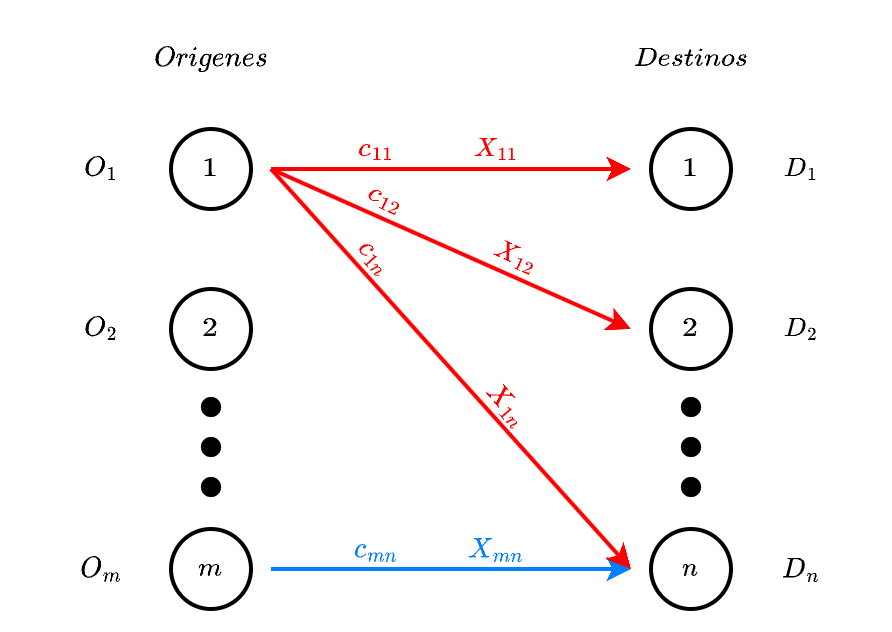
\includegraphics[scale=0.15]{diagram/ProblemaTransporte.png}
\end{figure}
Donde:
\begin{itemize}
    \item m: Origenes con oferta $O_i$.
    \item n: Destinos con demanda $D_j$.
    \item $C_{ij}$: Costos unitarios de transportar desde i hasta j.
    \item $X_{ij}$: Variables de decisión, cantidad de unidades a transportar desde i hasta j. \textcolor{red!50}{(m-n)}
    \item \textbf{Objetivo}: Minimizar costo total de transporte. S.T restricciones. \textcolor{blue!50}{(m+n)} 
\end{itemize}

\subsubsection*{Modelo Lineal}

\begin{figure}[H]
    \centering
    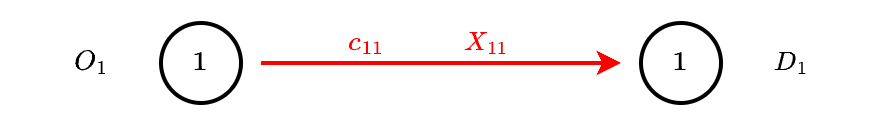
\includegraphics[scale=0.15]{diagram/ModeloLineal.png}
\end{figure}
\begin{equation*}
    c_{11} \times X_{11} = \text{Costo total de 1 a 1}
\end{equation*}

\subsubsection*{Funcion Objetivo:}
\begin{align*}
    \text{Min} \quad Z &= c_{11} \times X_{11} + c_{12} \times X_{12} + ... + c_{mn} \times X_{mn} \\
    \text{Min} \quad Z &= \sum_{i=1}^{m}{\sum_{j=1}^{n}{c_{ij} \times X_{ij}}}
\end{align*}

\newpage
\subsubsection*{Restricciones Ofertas:}
\begin{figure}[H]
    \centering
    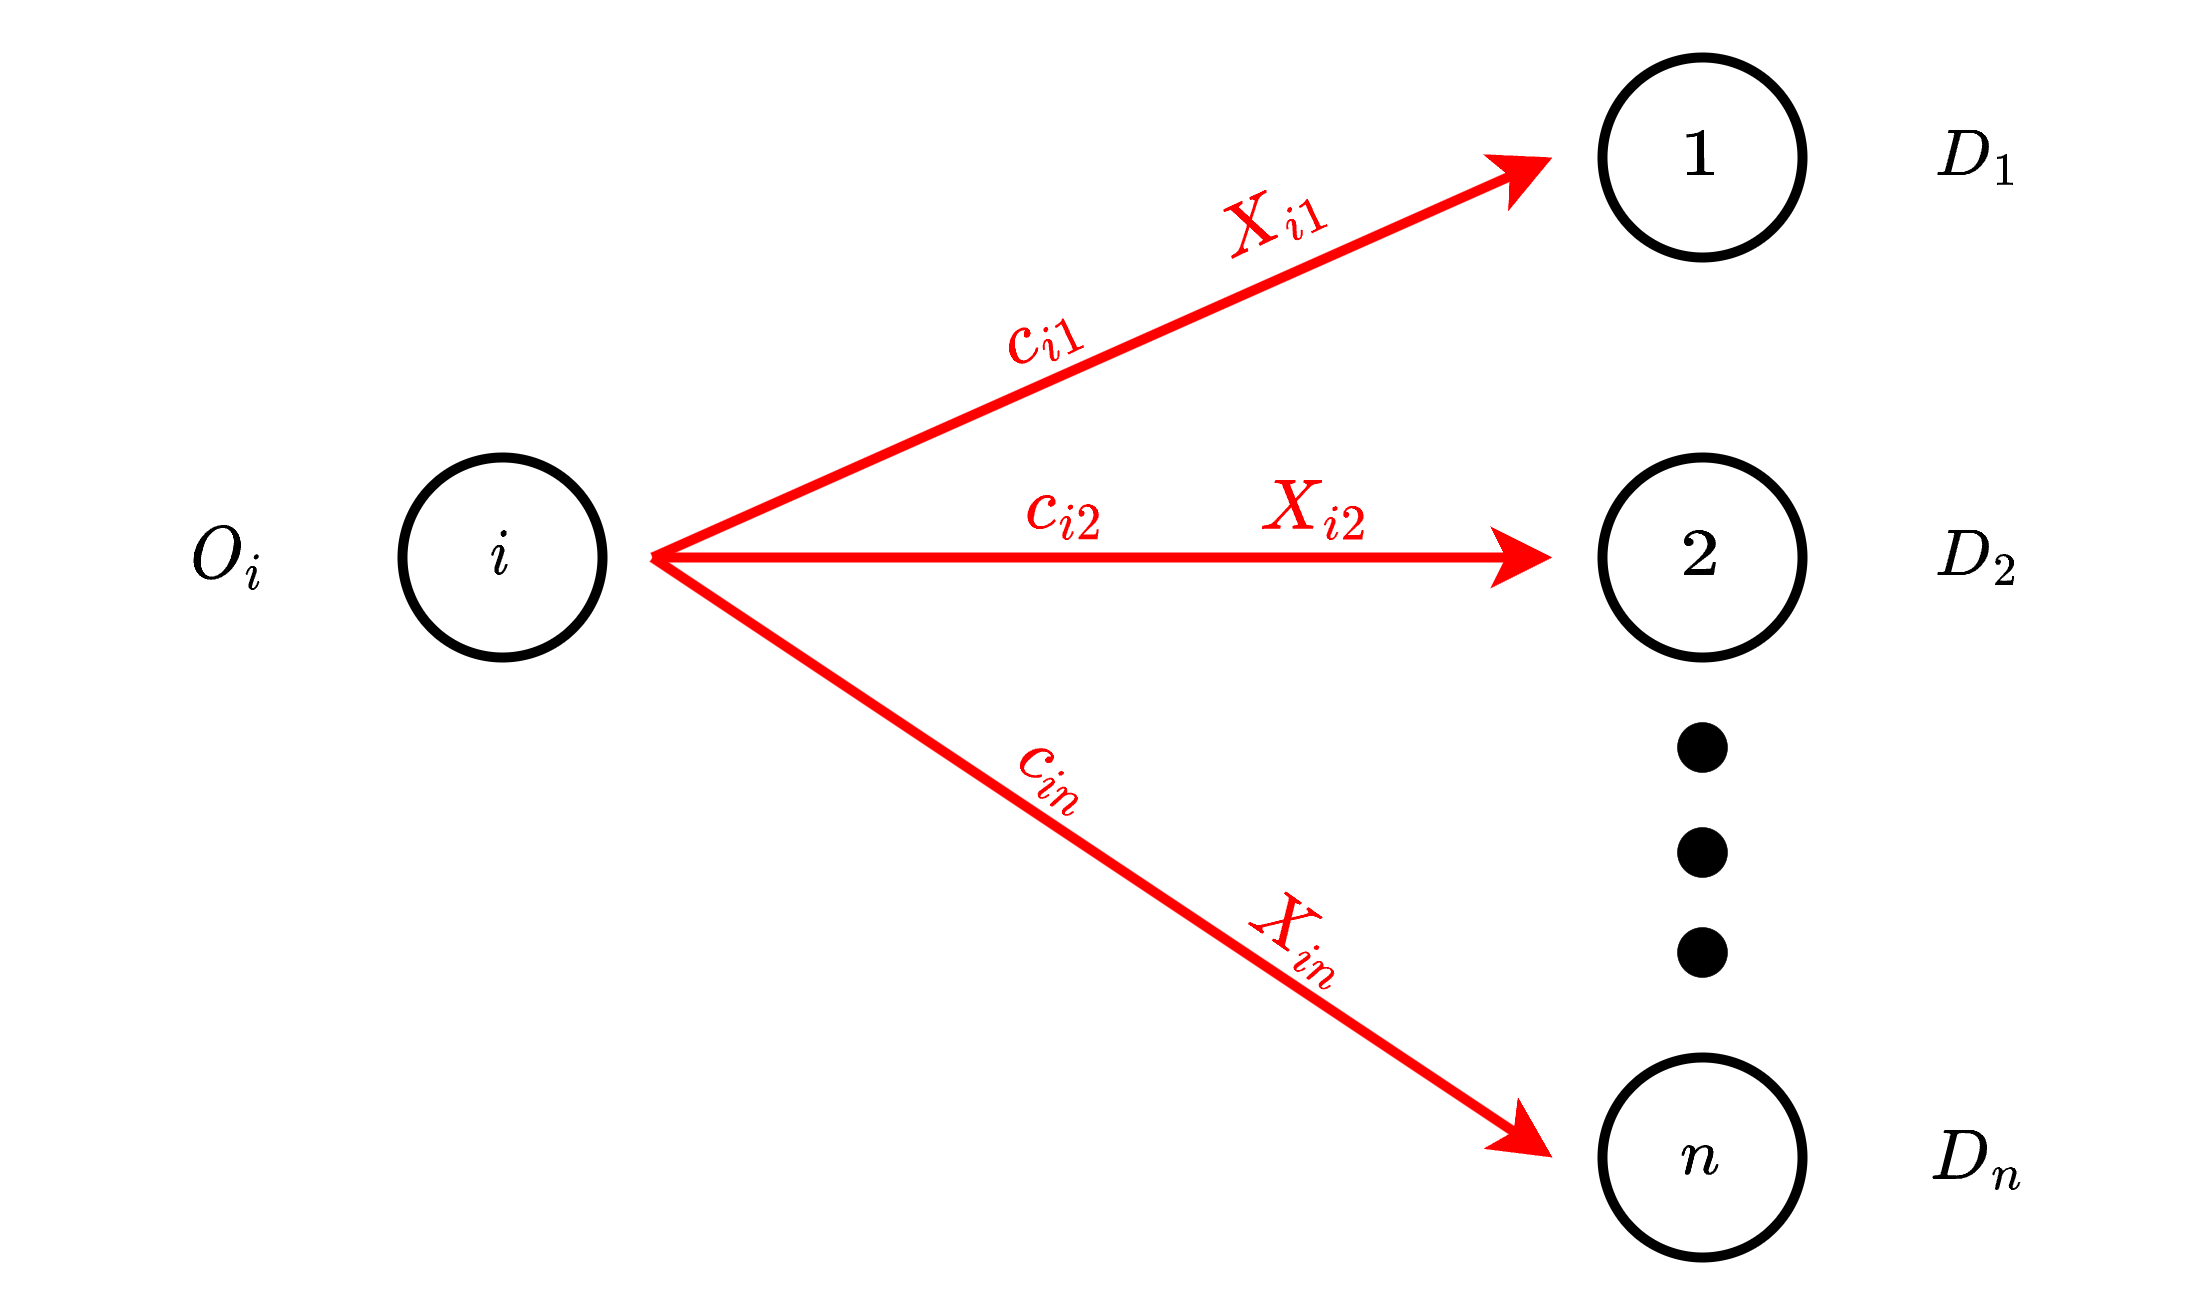
\includegraphics[scale=0.15]{diagram/RestriccionesOferta.png}
\end{figure}
\begin{align*}
    x_{i1} + x_{i2} + ... + x_{in} \leq O_i \quad \forall i = \overline{1,m}
\end{align*}
\begin{equation*}
    \sum_{j=1}^{n}{X_{ij}} \leq O_i \quad \forall i = \overline{1,m}
\end{equation*}

\subsubsection*{Restricciones Demandas:}
\begin{figure}[H]
    \centering
    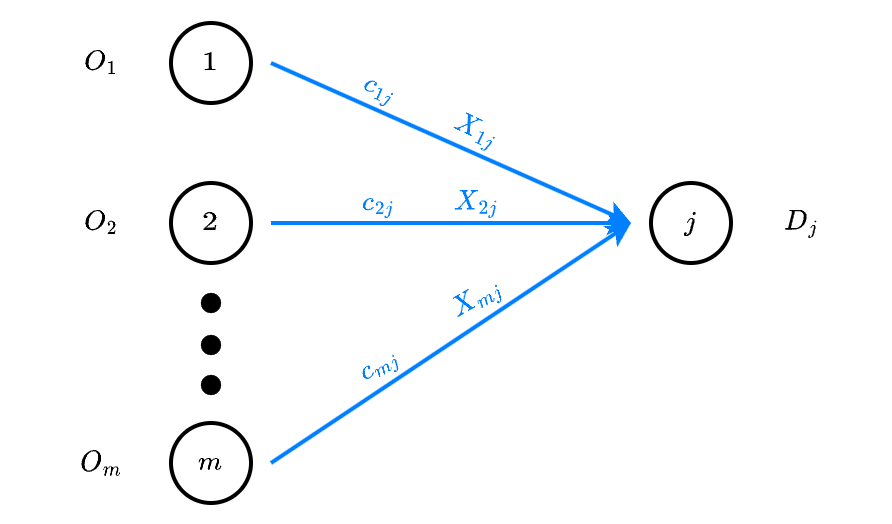
\includegraphics[scale=0.15]{diagram/RestriccionesDemanda.png}
\end{figure}
\begin{align*}
    x_{1j} + x_{2j} + ... + x_{mj} \geq D_j \quad \forall j = \overline{1,n}
\end{align*}
\begin{equation*}
    \sum_{i=1}^{m}{X_{ij}} \geq D_j \quad \forall j = \overline{1,n}
\end{equation*}

\newpage
\subsubsection*{En resumen:}
Los P.T. quedan de la forma:
\begin{align*}
    \text{Min} \quad Z &= \sum_{i=1}^{m}{\sum_{j=1}^{n}{c_{ij} \times X_{ij}}} \\
    \text{s.a} \quad & \sum_{j=1}^{n}{X_{ij}} \leq O_i \quad \forall i = \overline{1,m} \\
    & \sum_{i=1}^{m}{X_{ij}} \geq D_j \quad \forall j = \overline{1,n} \\
    & X_{ij} \geq 0 \quad \forall i = \overline{1,m}, \forall j = \overline{1,n}
\end{align*}

\subsection*{Problema 10: Problema de transporte}
Escribir el M.L. para el siguiente P.T.:
\begin{figure}[H]
    \centering
    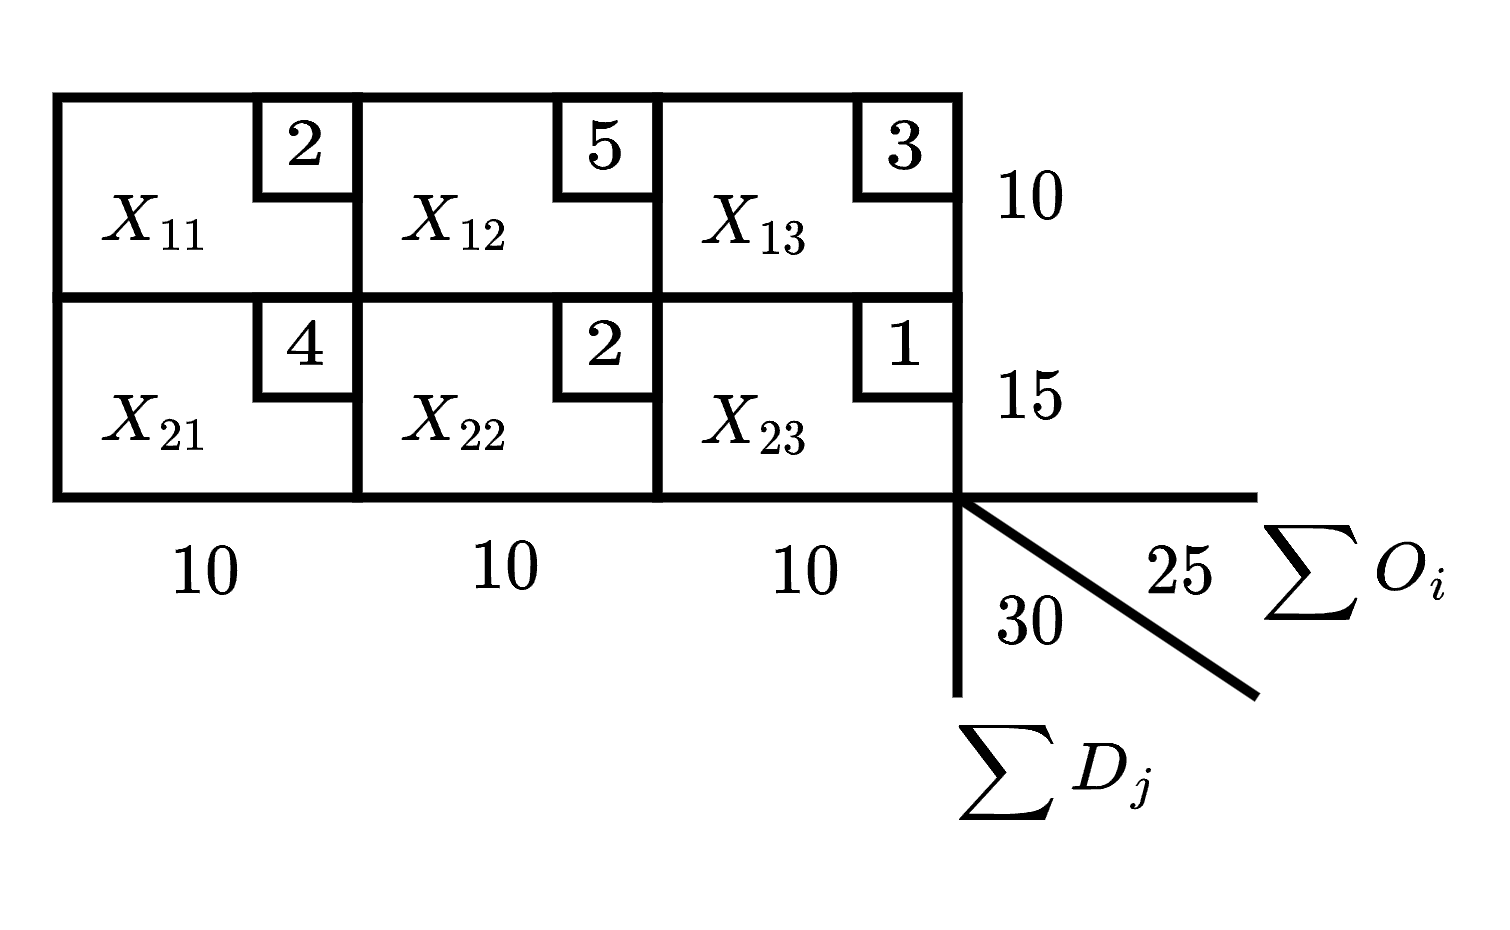
\includegraphics[scale=0.15]{diagram/PTE1.png}
\end{figure}

\subsubsection*{Función Objetivo:}
\begin{equation*}
    \begin{aligned}
        \text{Min} \quad & Z = 2X_{11} + 5X_{12} + 3X_{13} + 4X_{21} + 2X_{22} + X_{23}\\
        \text{s.a} \quad & X_{11} + X_{12} + X_{13} \leq 10 \\
        & X_{21} + X_{22} + X_{23} \leq 15 \\
        & X_{11} + X_{21} \geq 10 \\
        & X_{12} + X_{22} \geq 10 \\
        & X_{13} + X_{23} \geq 10 \\
        & X_{ij} \geq 0 \quad \forall i = \overline{1,2}, \forall j = \overline{1,4}
    \end{aligned}
\end{equation*}
\begin{itemize}
    \item Si en un P.T. $\sum{D_j} = \sum{O_i}$, diremos que el P.T. \underline{esta balanceado}.
\end{itemize}

\newpage
\begin{itemize}
    \item Si un P.T. \underline{esta desbalanceado} se puede balancear incorporando una restricción con coeficientes de costo nulo.
\end{itemize}
\begin{figure}[H]
    \centering
    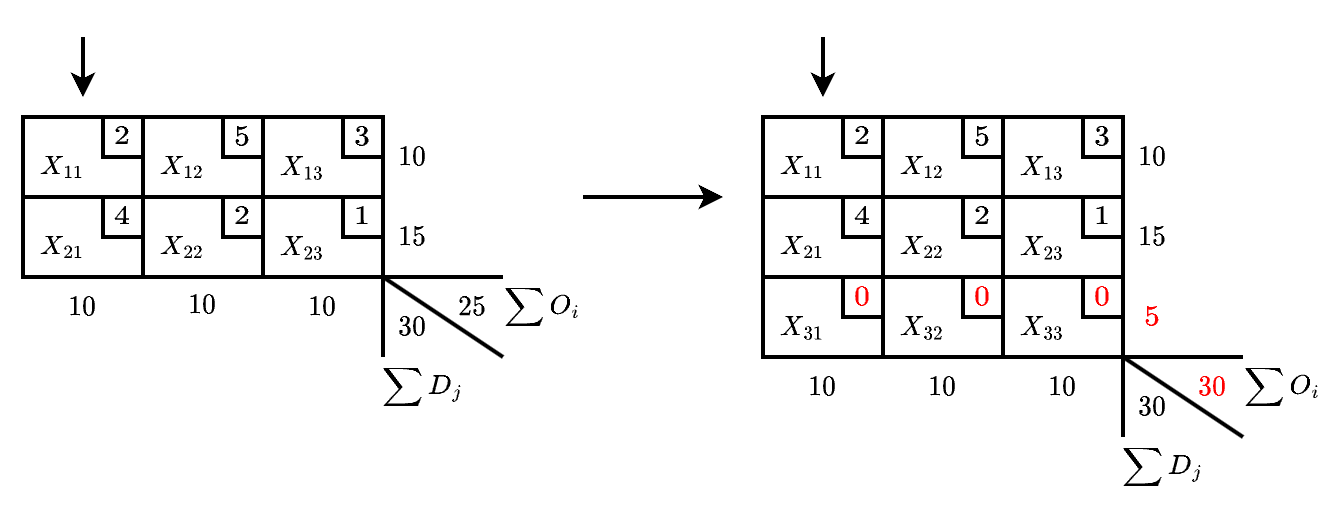
\includegraphics[scale=0.125]{diagram/PTE1B.png}
\end{figure}

\subsubsection*{Teorema}
En un P.T. balanceado, todas las restricciones son Activas.
\begin{itemize}
    \item Las soluciones basicas factibles tienen $m+n-1$ variables básicas.
\end{itemize}

\begin{equation*}
    \textbf{S.B.F.I.} = \left\{
        \begin{array}{l} \text{Regla Nor-Oeste} \\
            \text{Costo Mínimo} \\
            \text{Vogël}
        \end{array}
    \right.
\end{equation*}

\subsection*{Problema 11: Regla Nor-Oeste, Costo Mínimo y Vogël}
Sea el siguiente P.T.:
\begin{figure}[H]
    \centering
    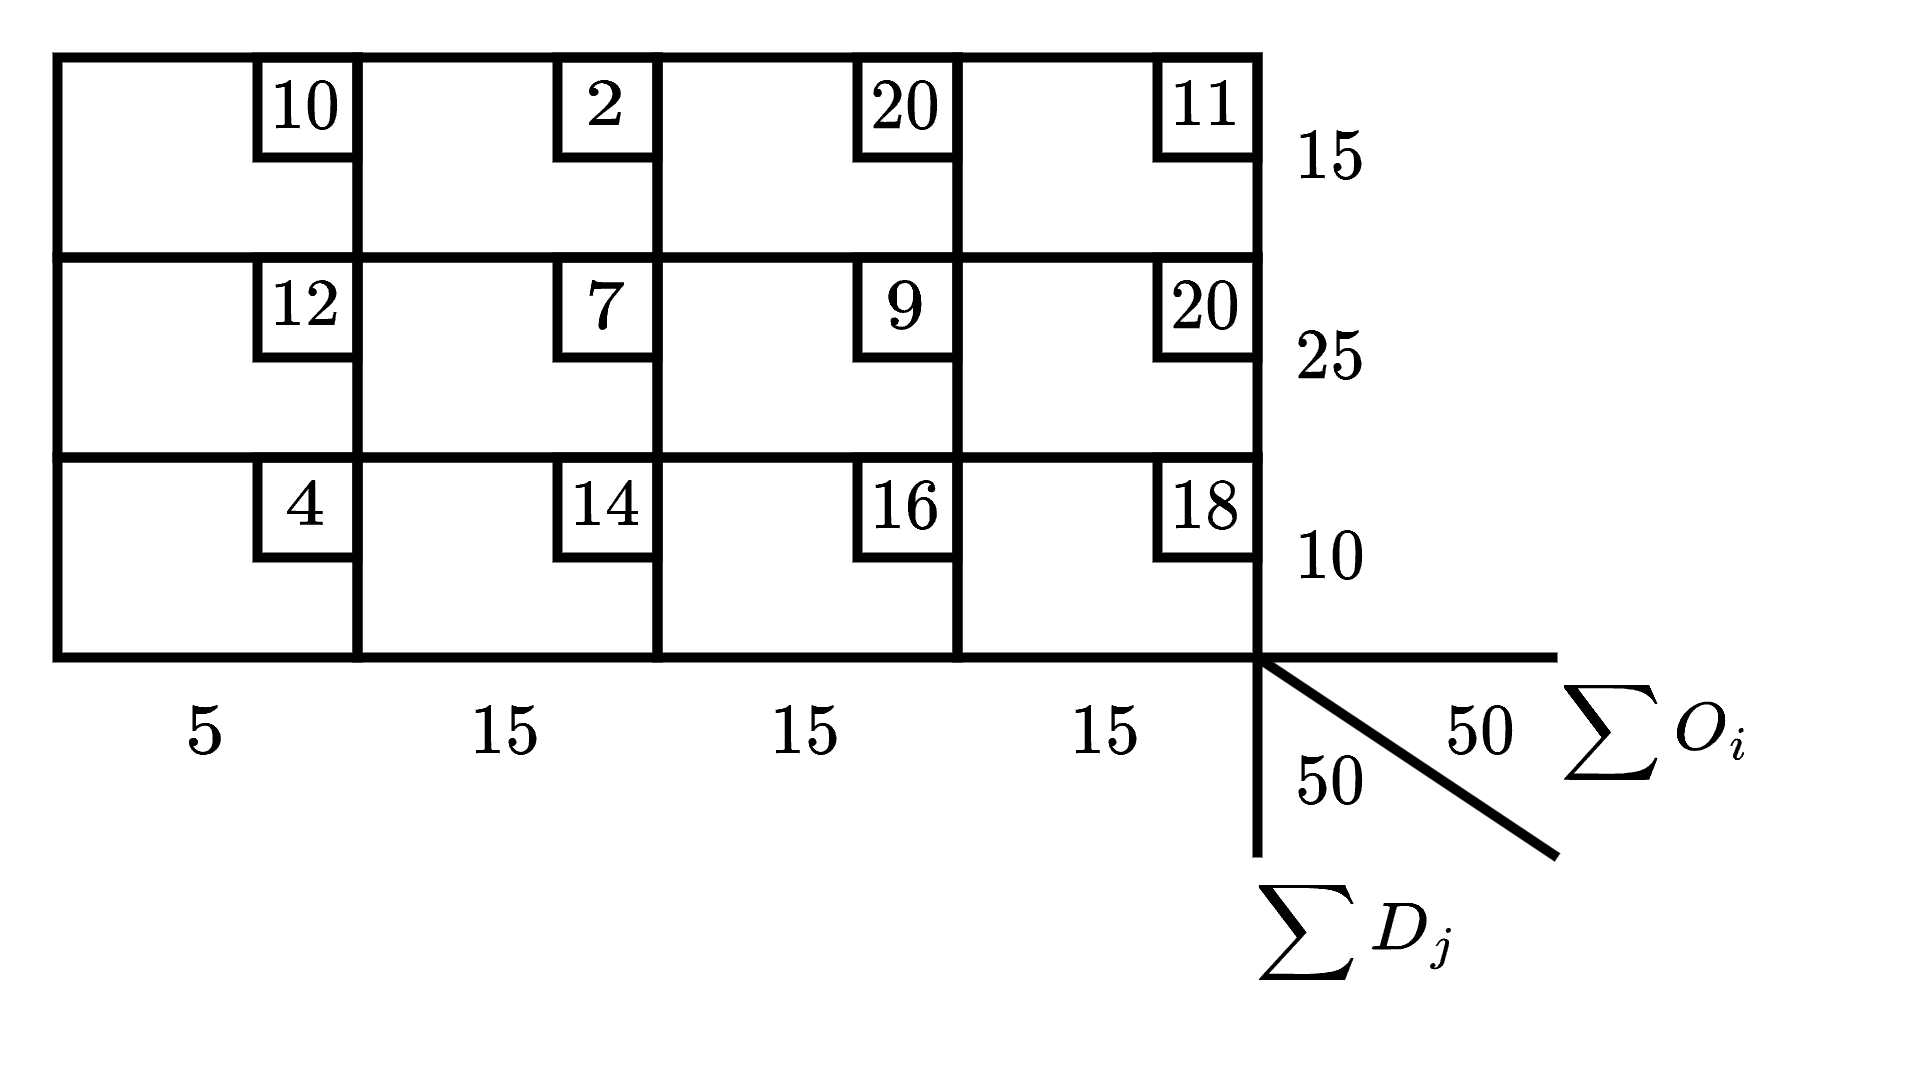
\includegraphics[scale=0.15]{diagram/PTE2RNO.png}
\end{figure}

\newpage
\subsubsection*{Por Regla Nor-Oeste}

Algoritmo:
\begin{itemize}
    \item Elegir una celda desde la esquina Nor-Oeste, le damos el máximo valor de oferta y demanda posible, para rellenar la fila y/o columna que no sea posible darle más.
    \begin{figure}[H]
        \centering
        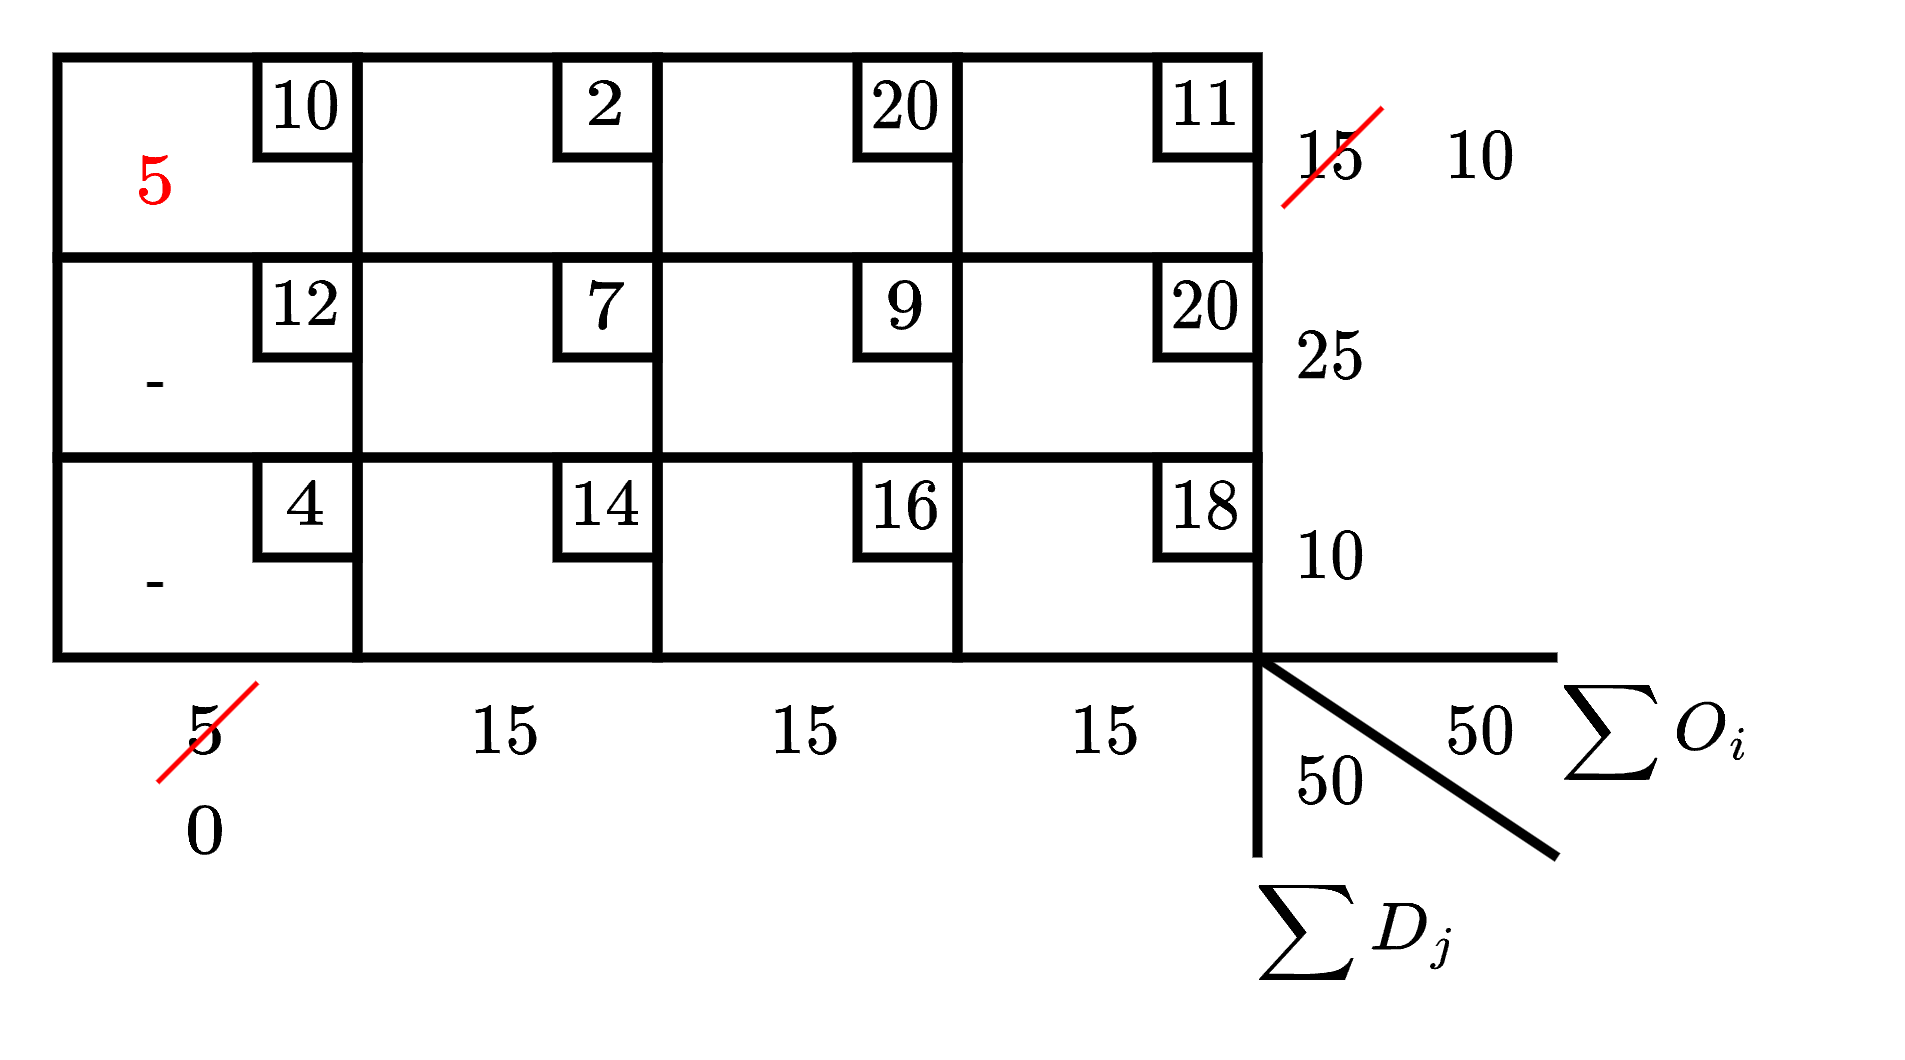
\includegraphics[scale=0.15]{diagram/PTE2RNO1.png}
    \end{figure}

    \item Repetimos hasta que se cumplan todas las restricciones.
    \begin{figure}[H]
        \centering
        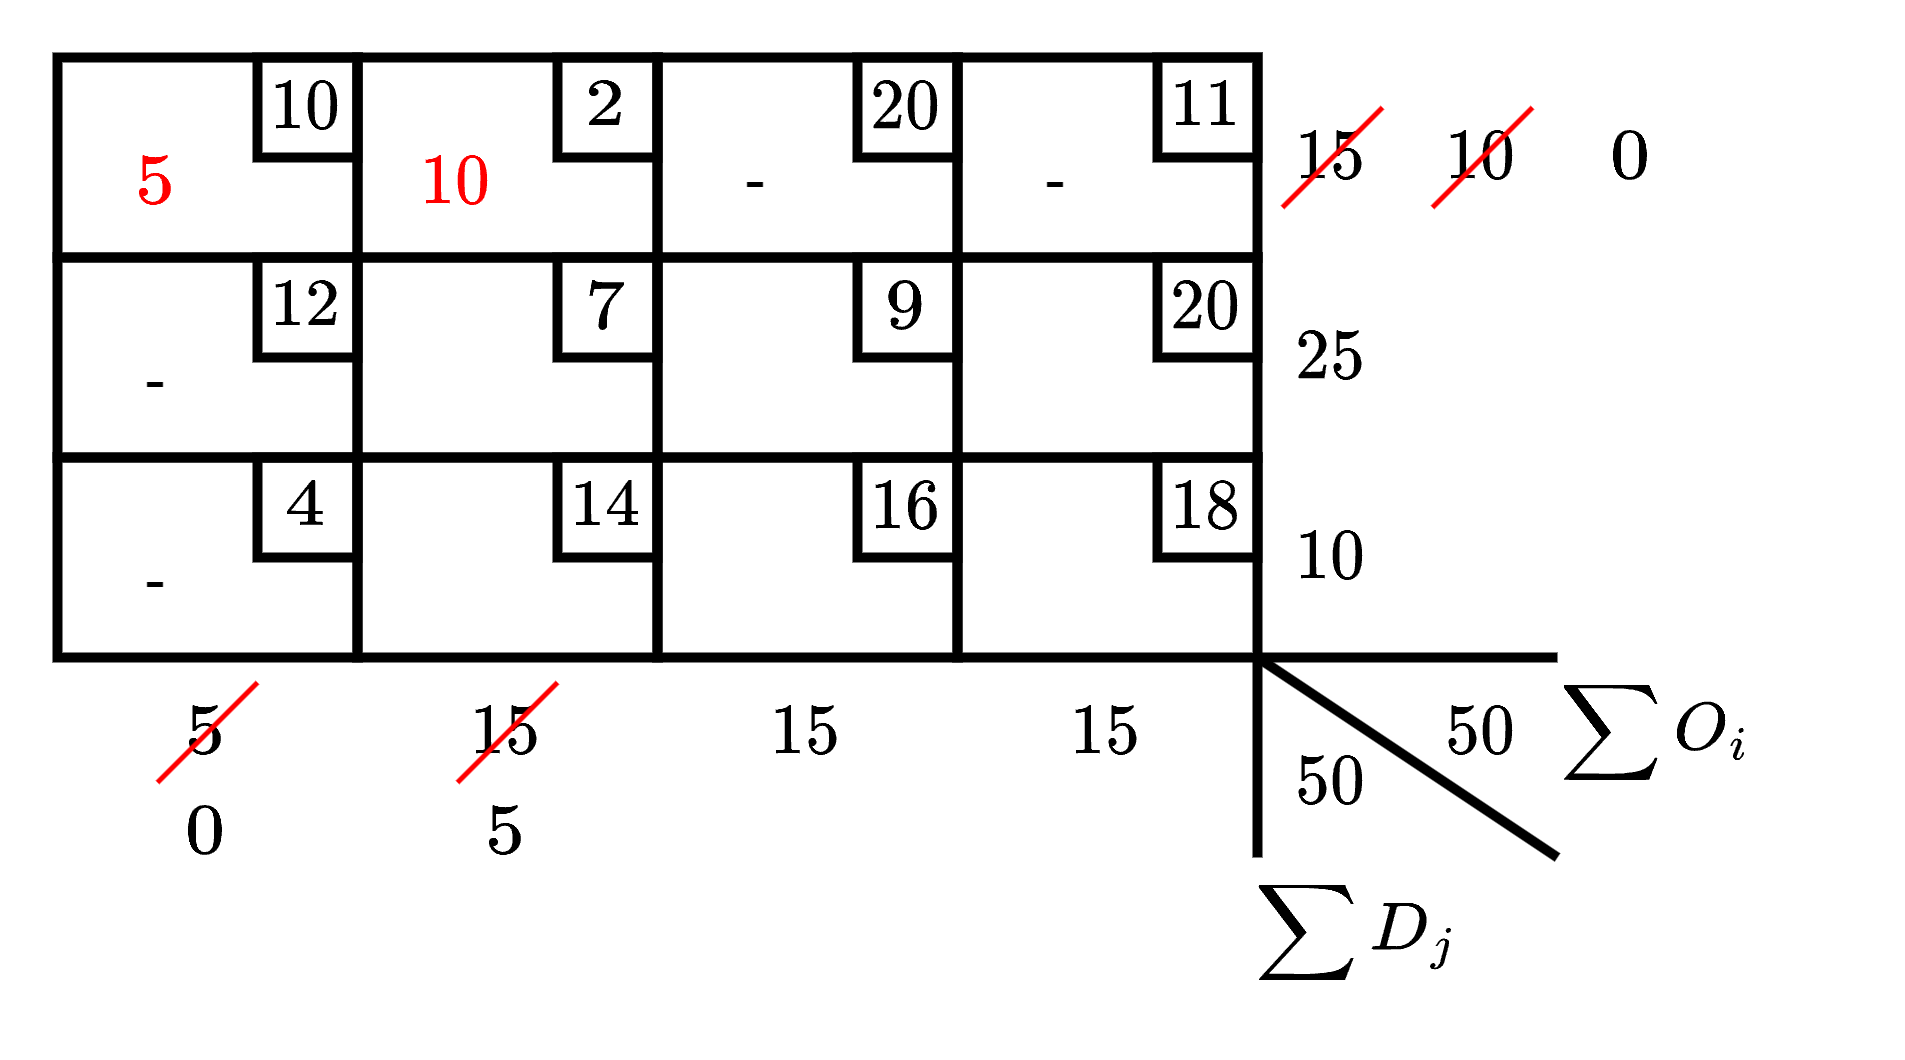
\includegraphics[scale=0.15]{diagram/PTE2RNO2.png}
    \end{figure}

    \begin{figure}[H]
        \centering
        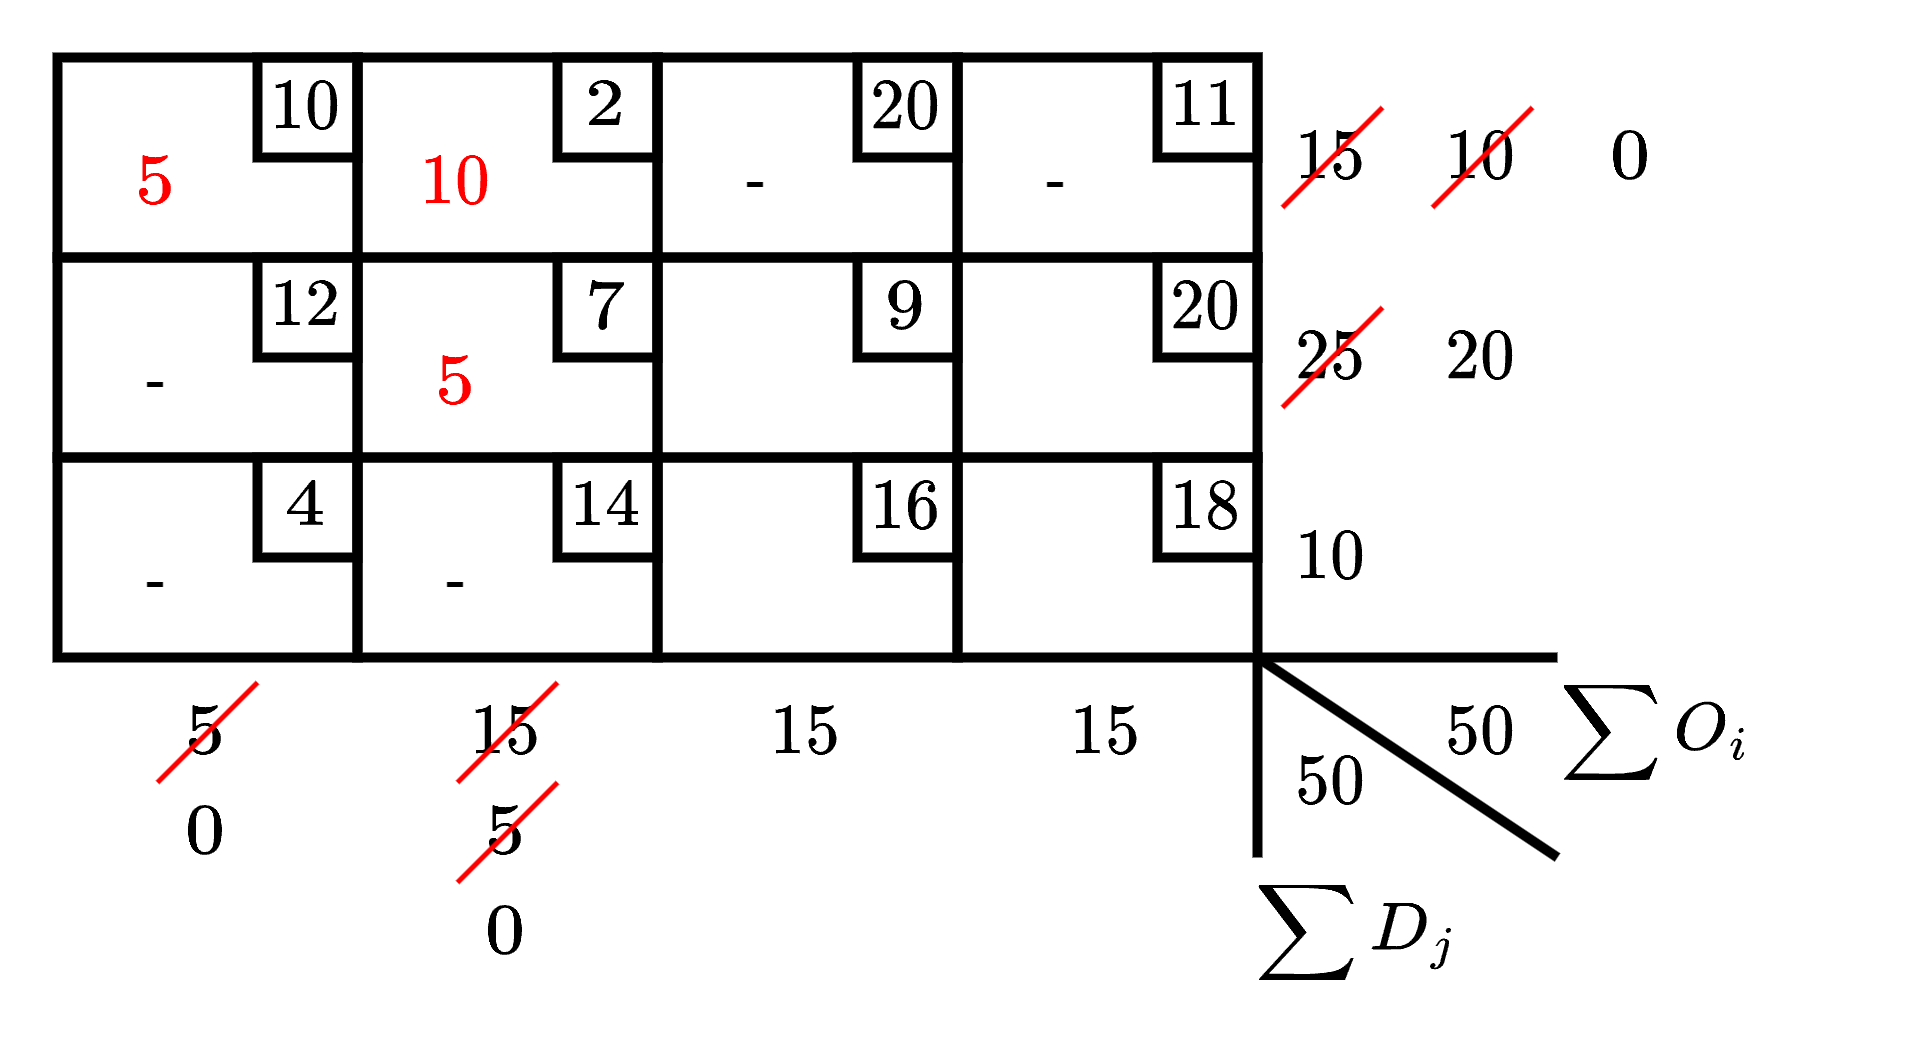
\includegraphics[scale=0.15]{diagram/PTE2RNO3.png}
    \end{figure}

    \begin{figure}[H]
        \centering
        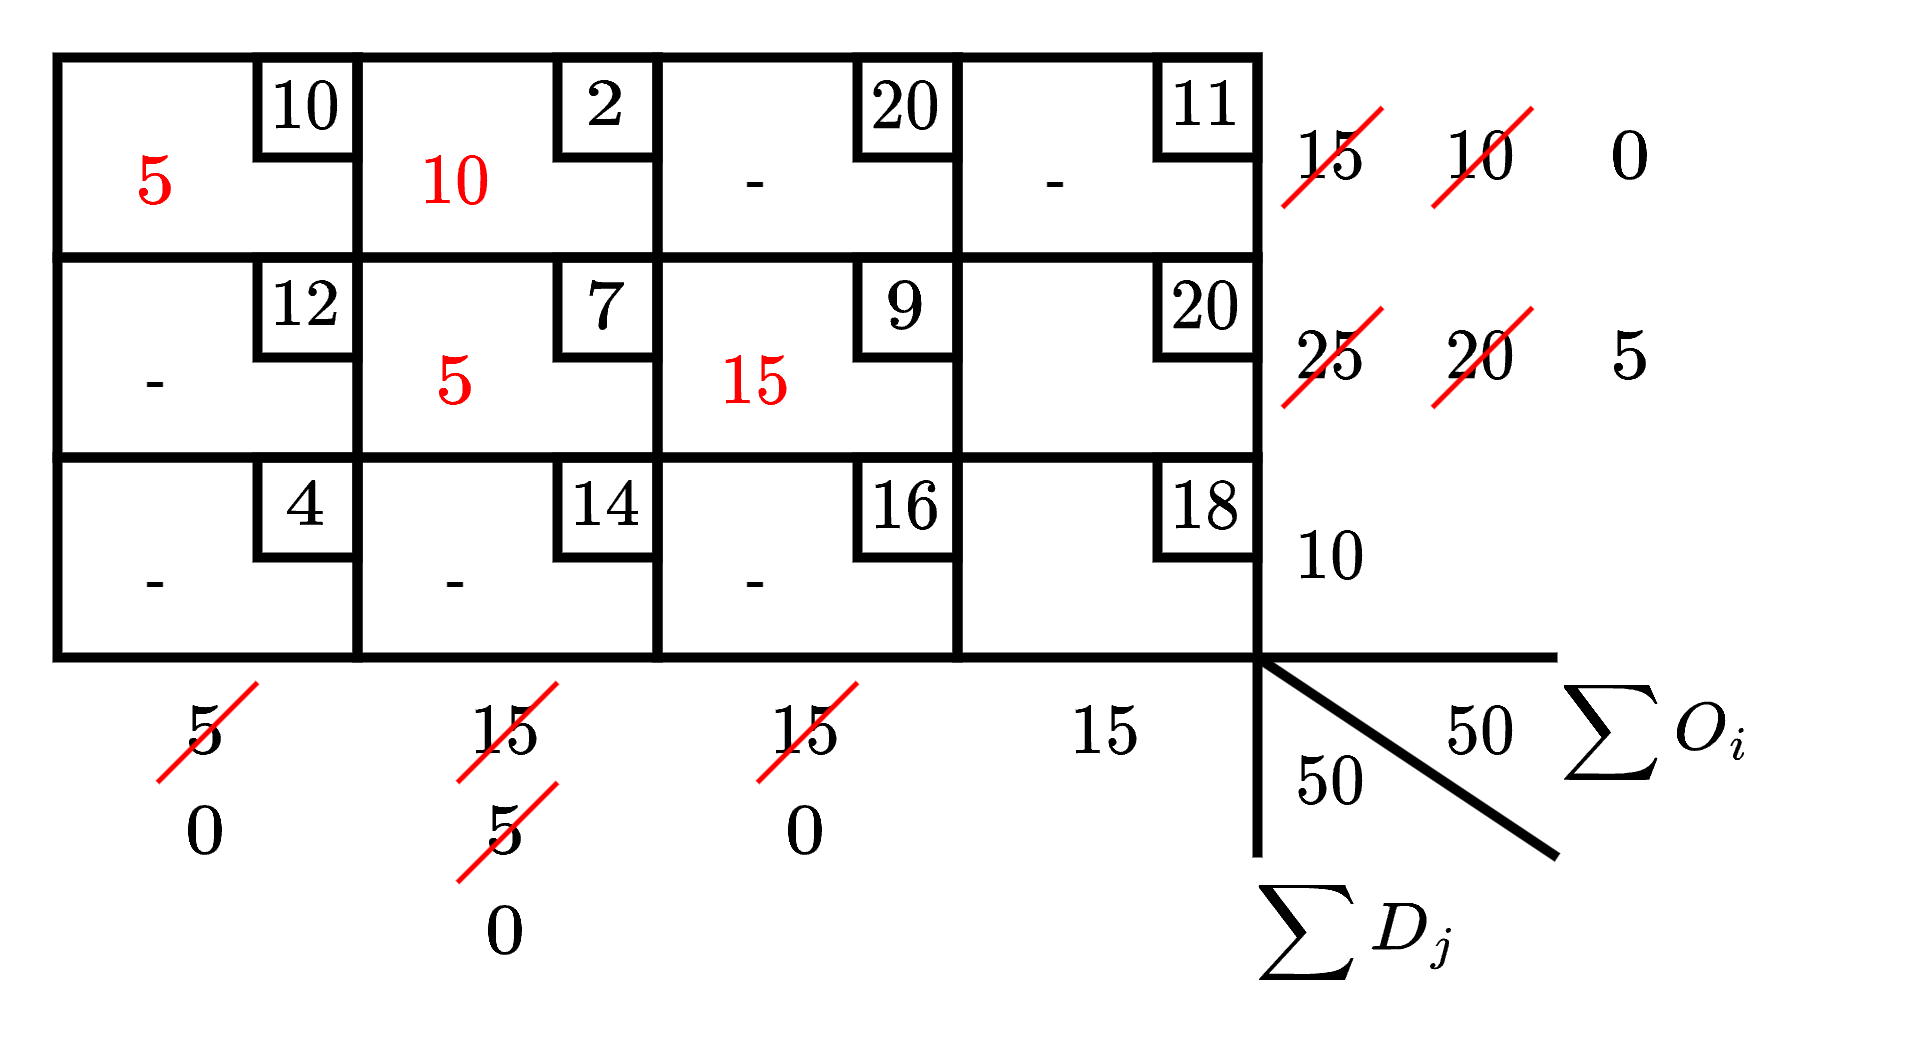
\includegraphics[scale=0.15]{diagram/PTE2RNO4.png}
    \end{figure}

    \begin{figure}[H]
        \centering
        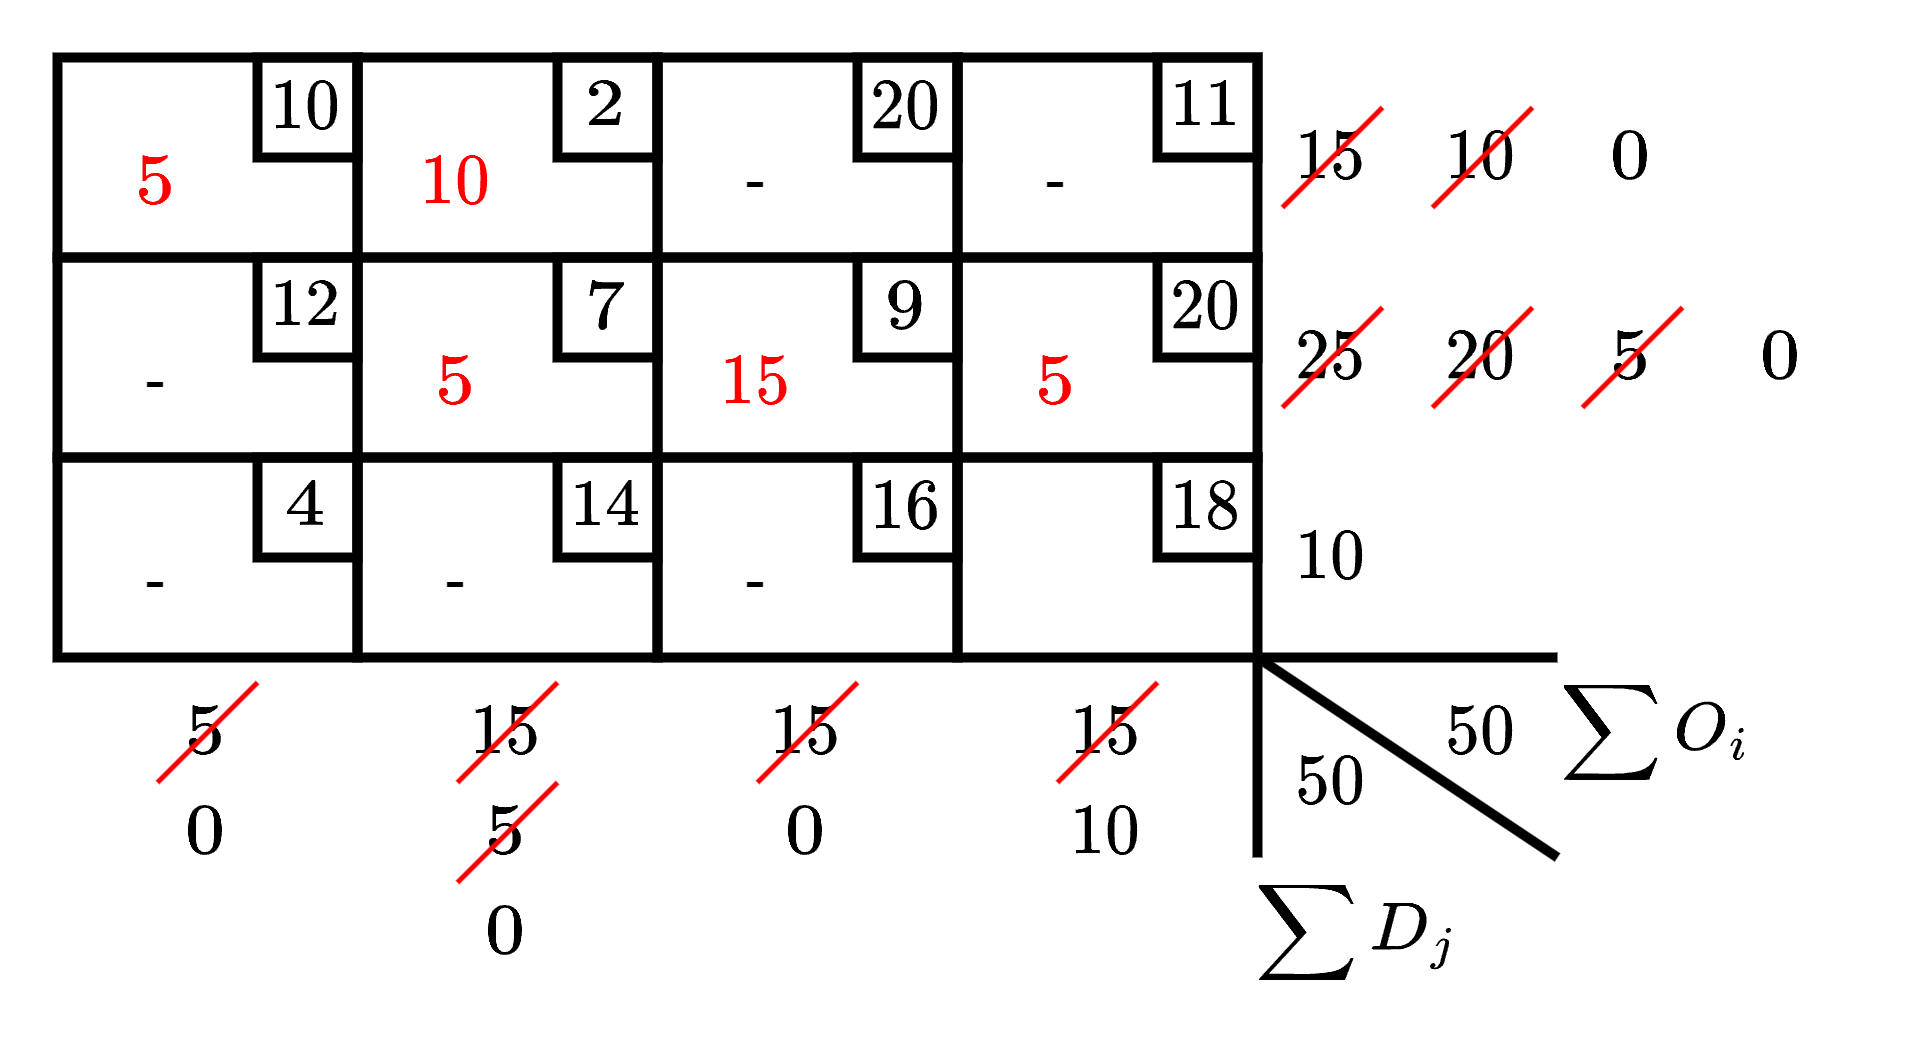
\includegraphics[scale=0.15]{diagram/PTE2RNO5.png}
    \end{figure}

    \begin{figure}[H]
        \centering
        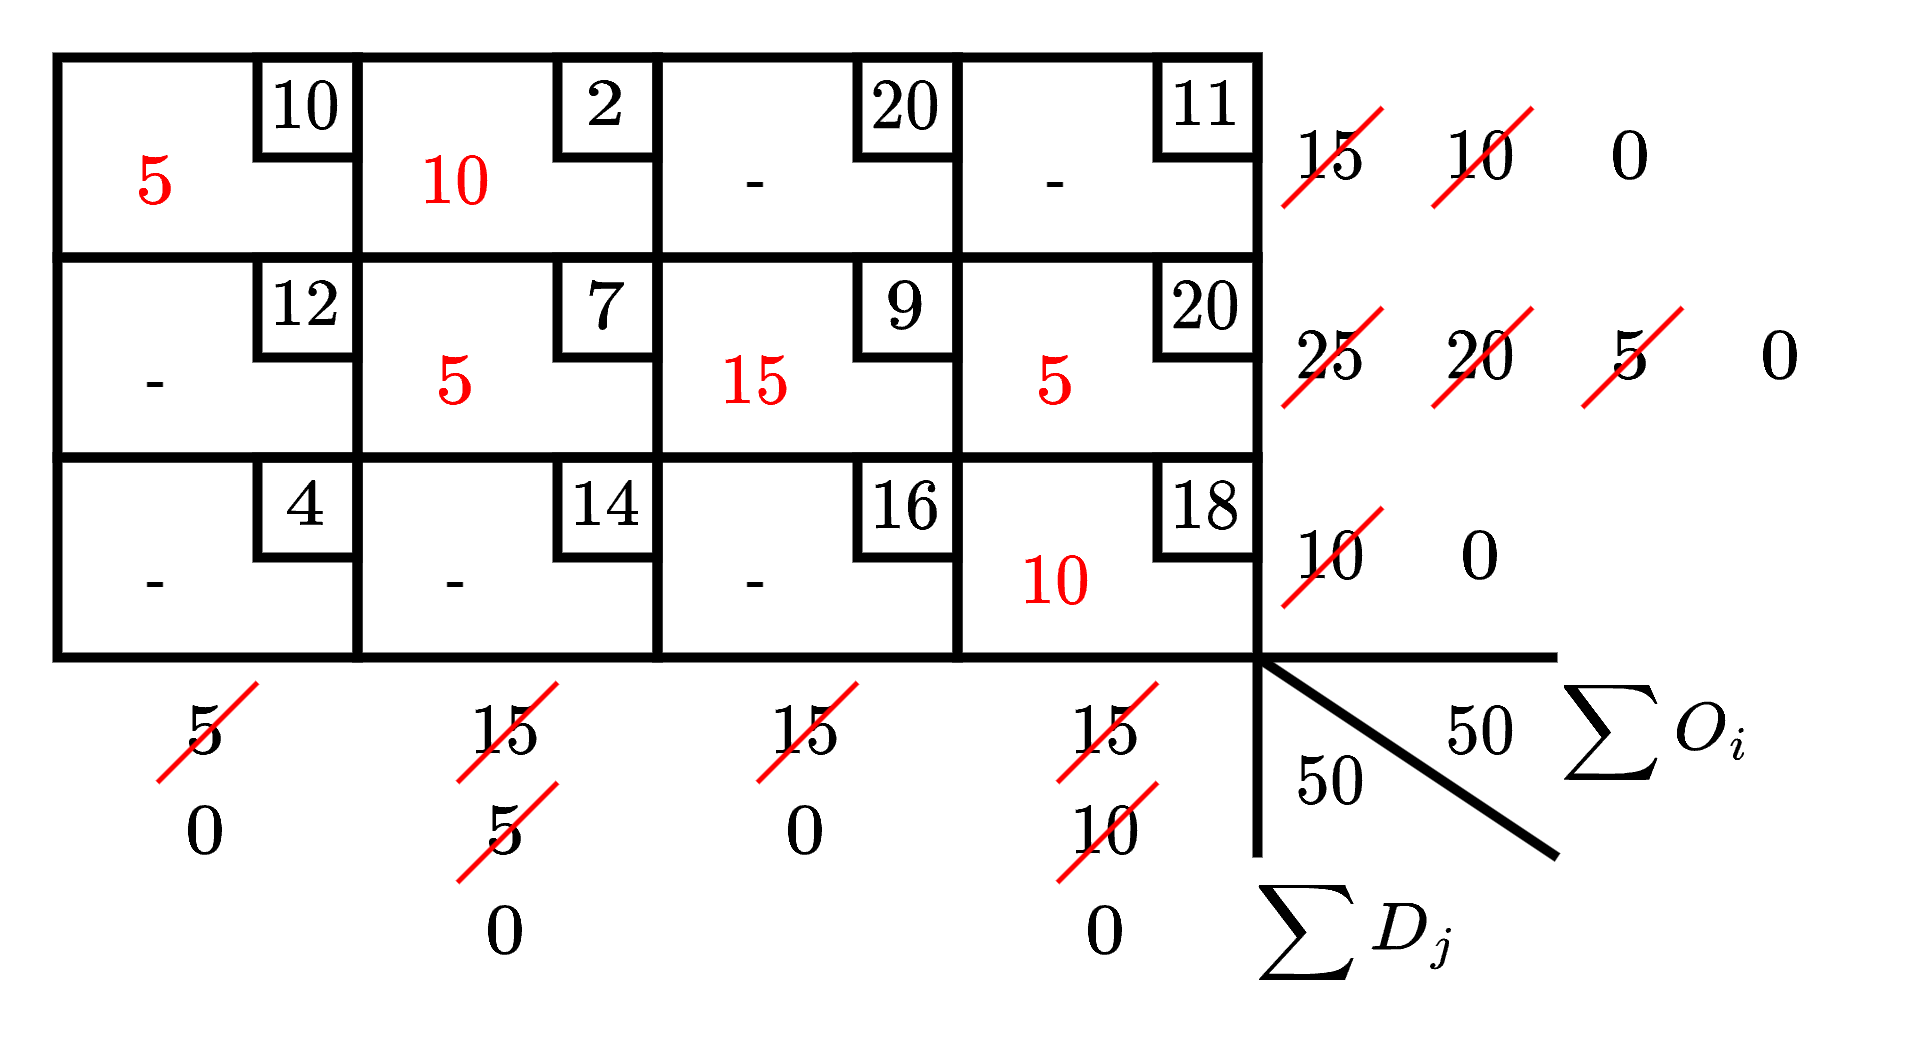
\includegraphics[scale=0.15]{diagram/PTE2RNO6.png}
    \end{figure}

    \item Verificamos la cantidad de soluciones factibles.
    \begin{equation*}
        \text{S.F.} = m+n-1 = 6
    \end{equation*}

    \item Calculamos el valor de la función objetivo.
    \begin{align*}
        Z &= 5 \cdot 10 + 10 \cdot 2 + 5 \cdot 7 + 15 \cdot 9 + 5 \cdot 20 + 10 \cdot 18 \\
        &= 50 + 20 + 35 + 135 + 100 + 180 \\
        &= 520 
    \end{align*}
\end{itemize}

\newpage
\subsubsection*{Por costo mínimo}
Algoritmo:
\begin{itemize}
    \item Elegimos el $c_{ij}$ más pequeño, le damos el valor maximo posible de oferta y demanda, luego elegimos fila o columna a rellenar con - de los demas $X_{ij}$.
    \begin{figure}[H]
        \centering
        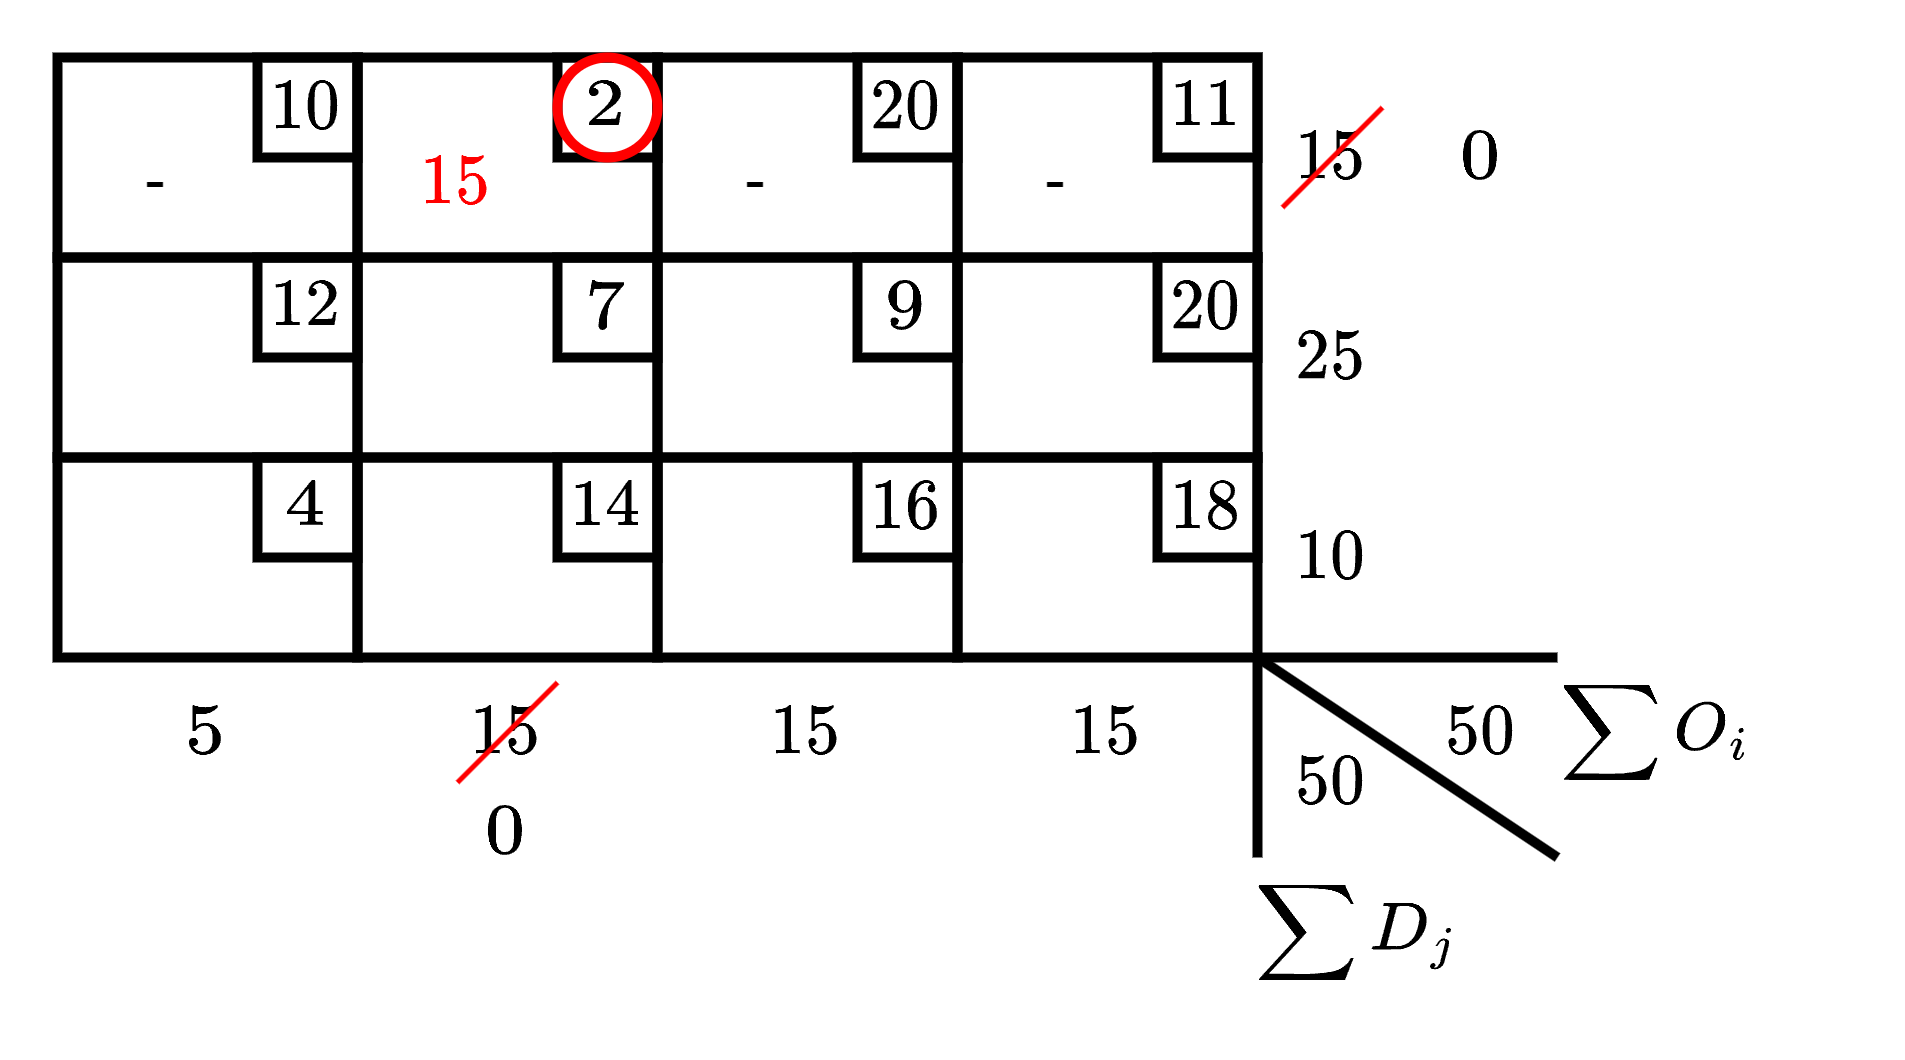
\includegraphics[scale=0.15]{diagram/PTE2CM1.png}
    \end{figure}
    
    \item Y repetimos lo anterior, hasta que se cumplan todas las restricciones.
    \begin{figure}[H]
        \centering
        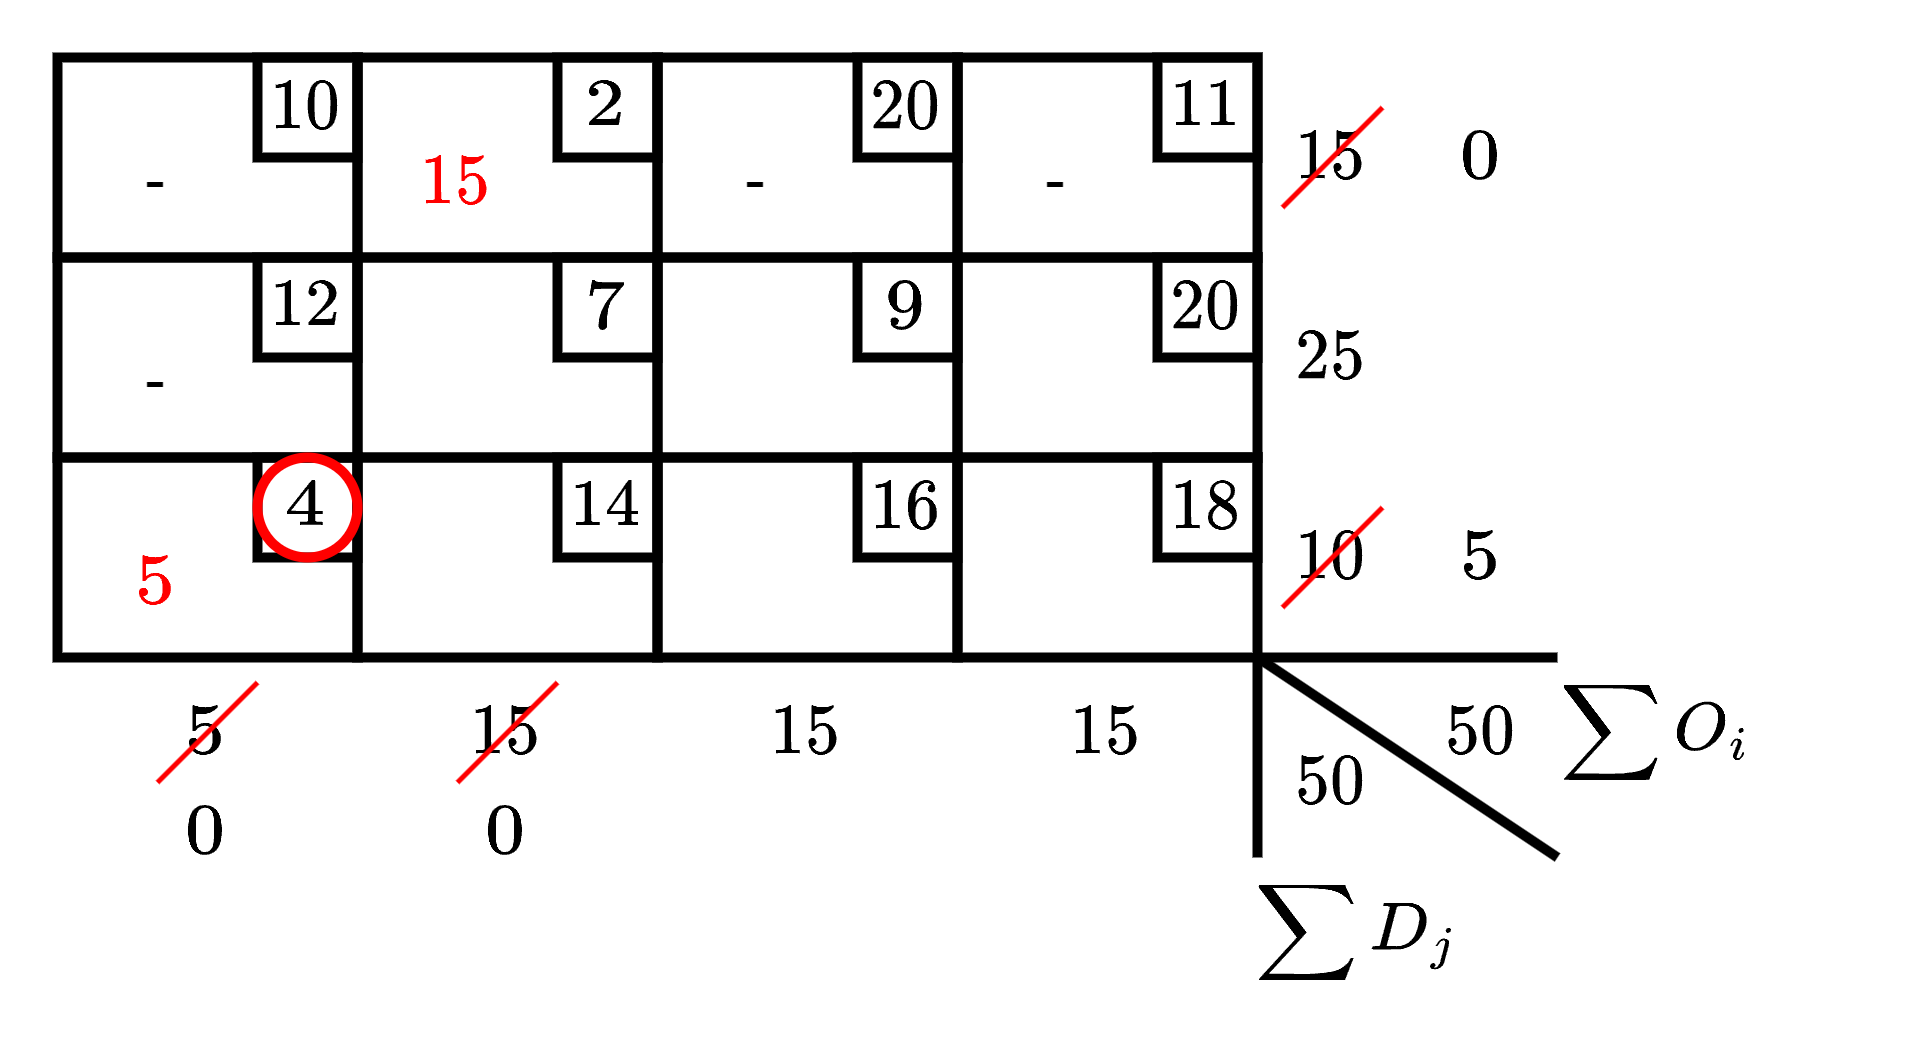
\includegraphics[scale=0.15]{diagram/PTE2CM2.png}
    \end{figure}

    \begin{figure}[H]
        \centering
        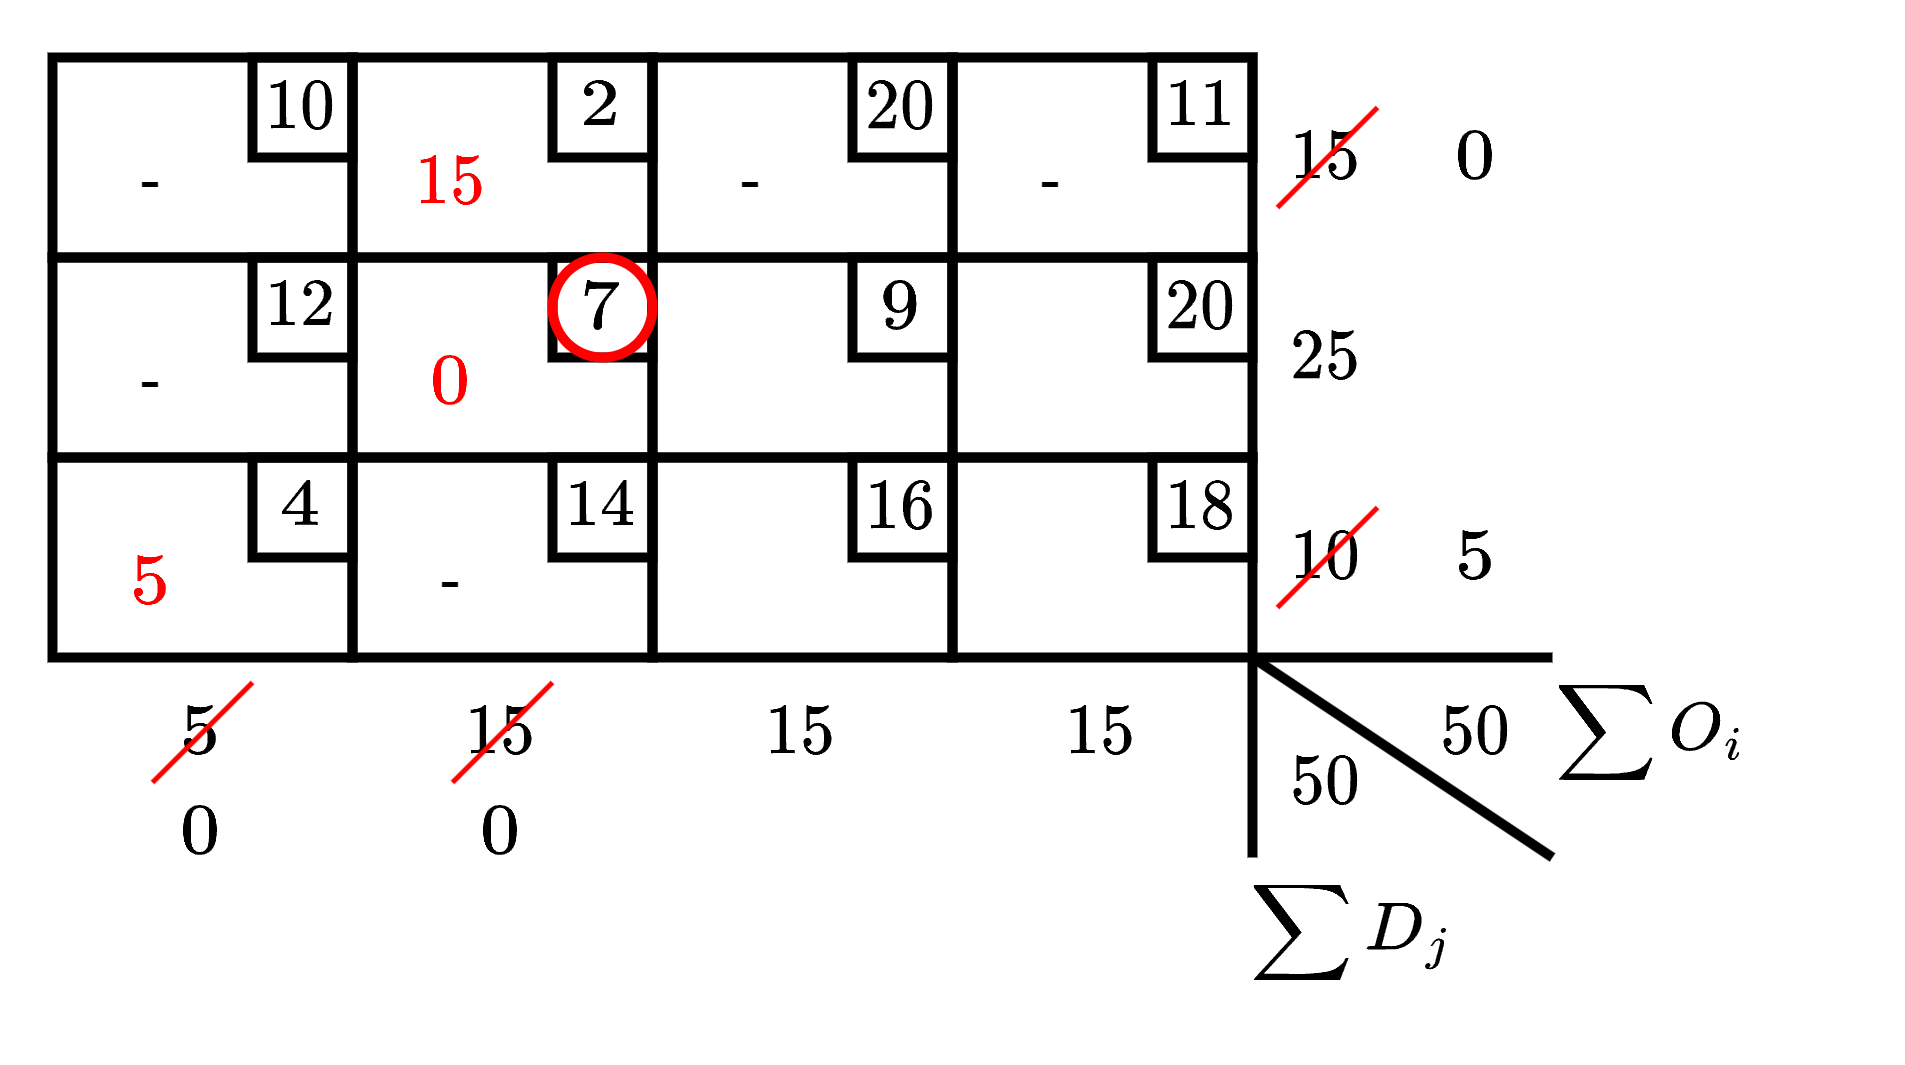
\includegraphics[scale=0.15]{diagram/PTE2CM3.png}
    \end{figure}

    \begin{figure}[H]
        \centering
        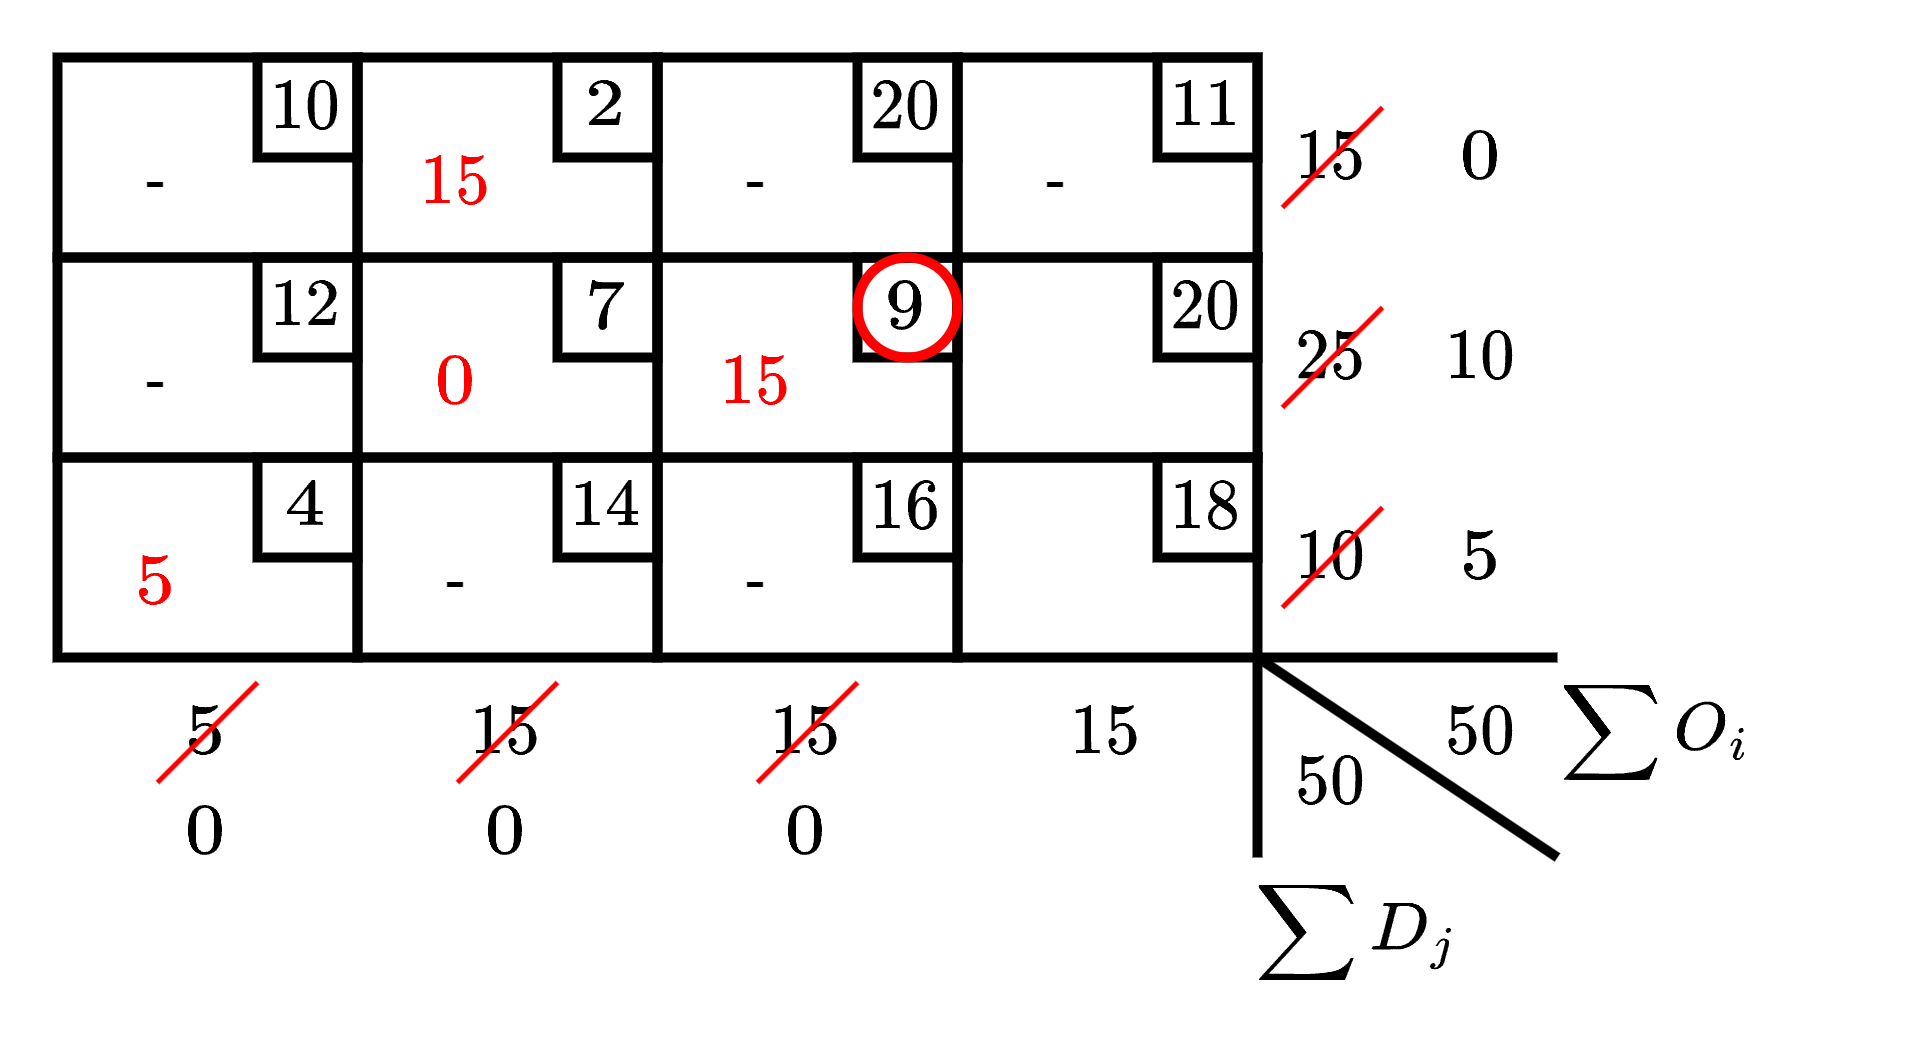
\includegraphics[scale=0.15]{diagram/PTE2CM4.png}
    \end{figure}
    
    \begin{figure}[H]
        \centering
        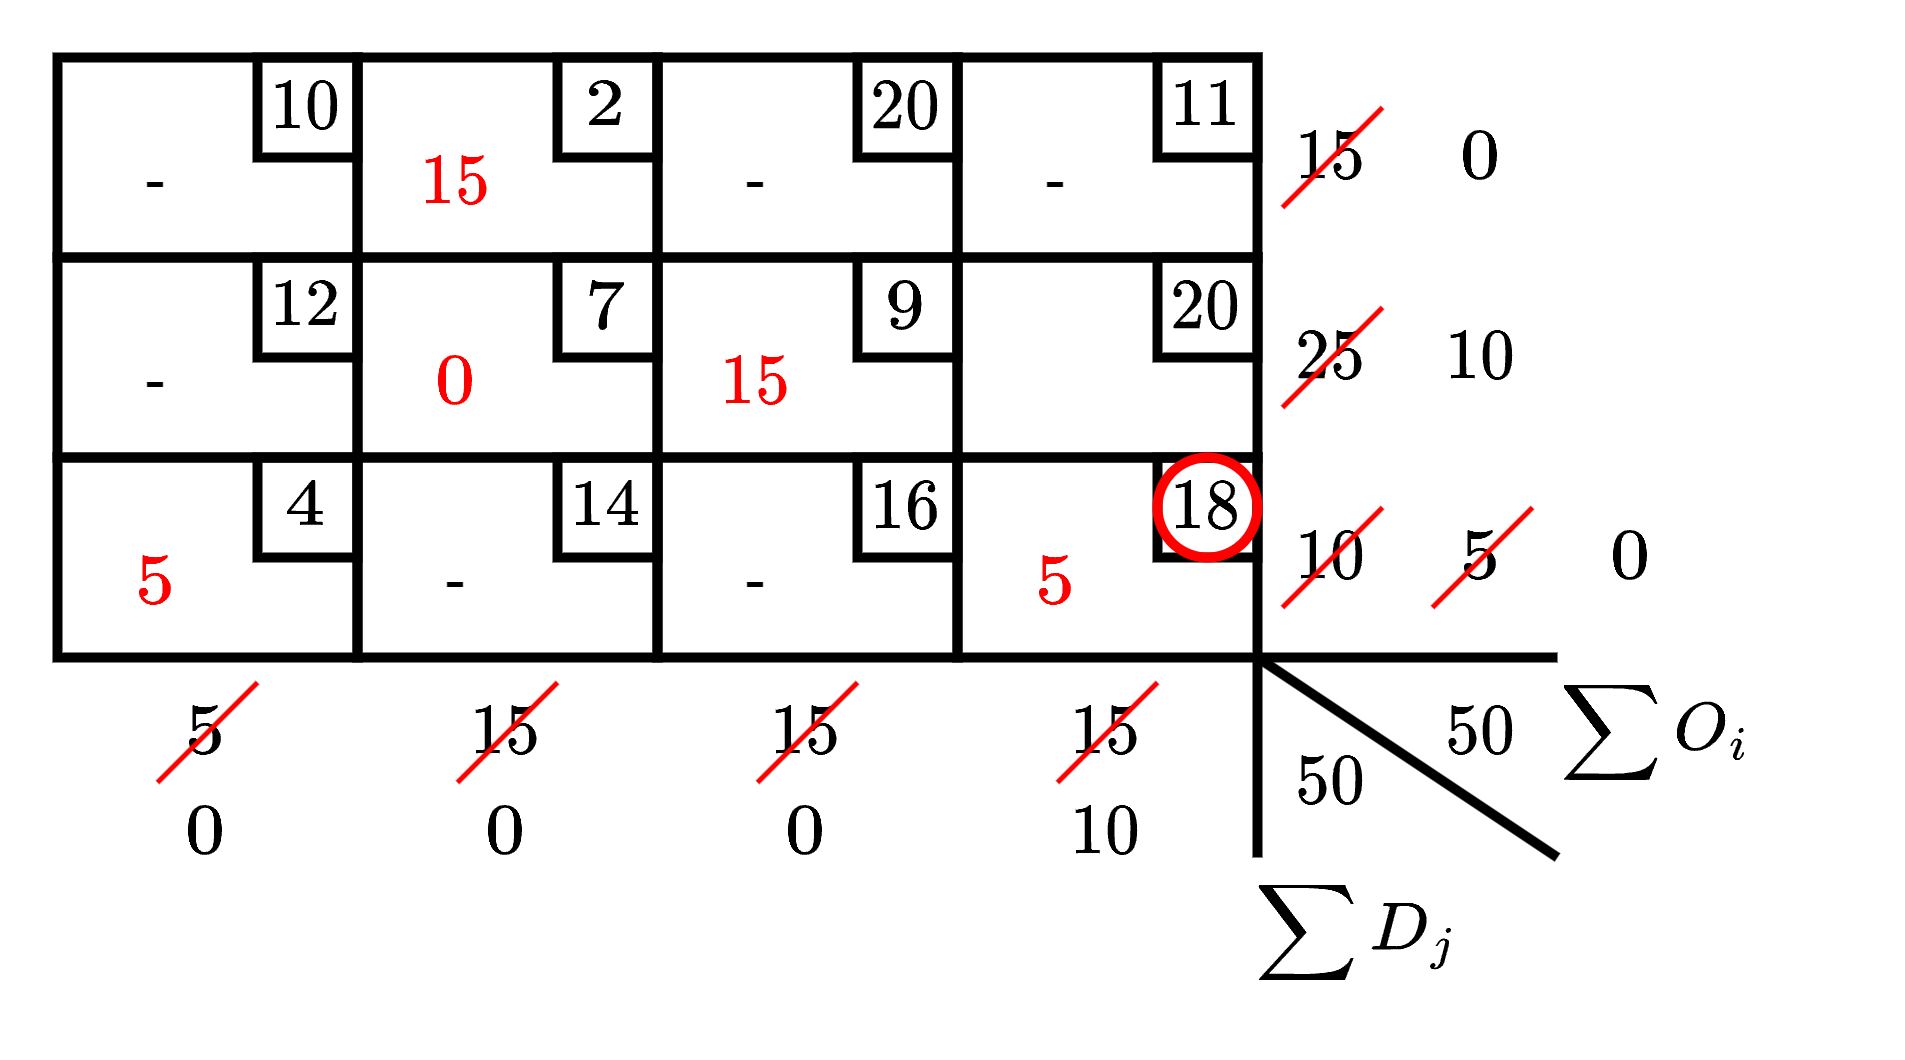
\includegraphics[scale=0.15]{diagram/PTE2CM5.png}
    \end{figure}
    
    \begin{figure}[H]
        \centering
        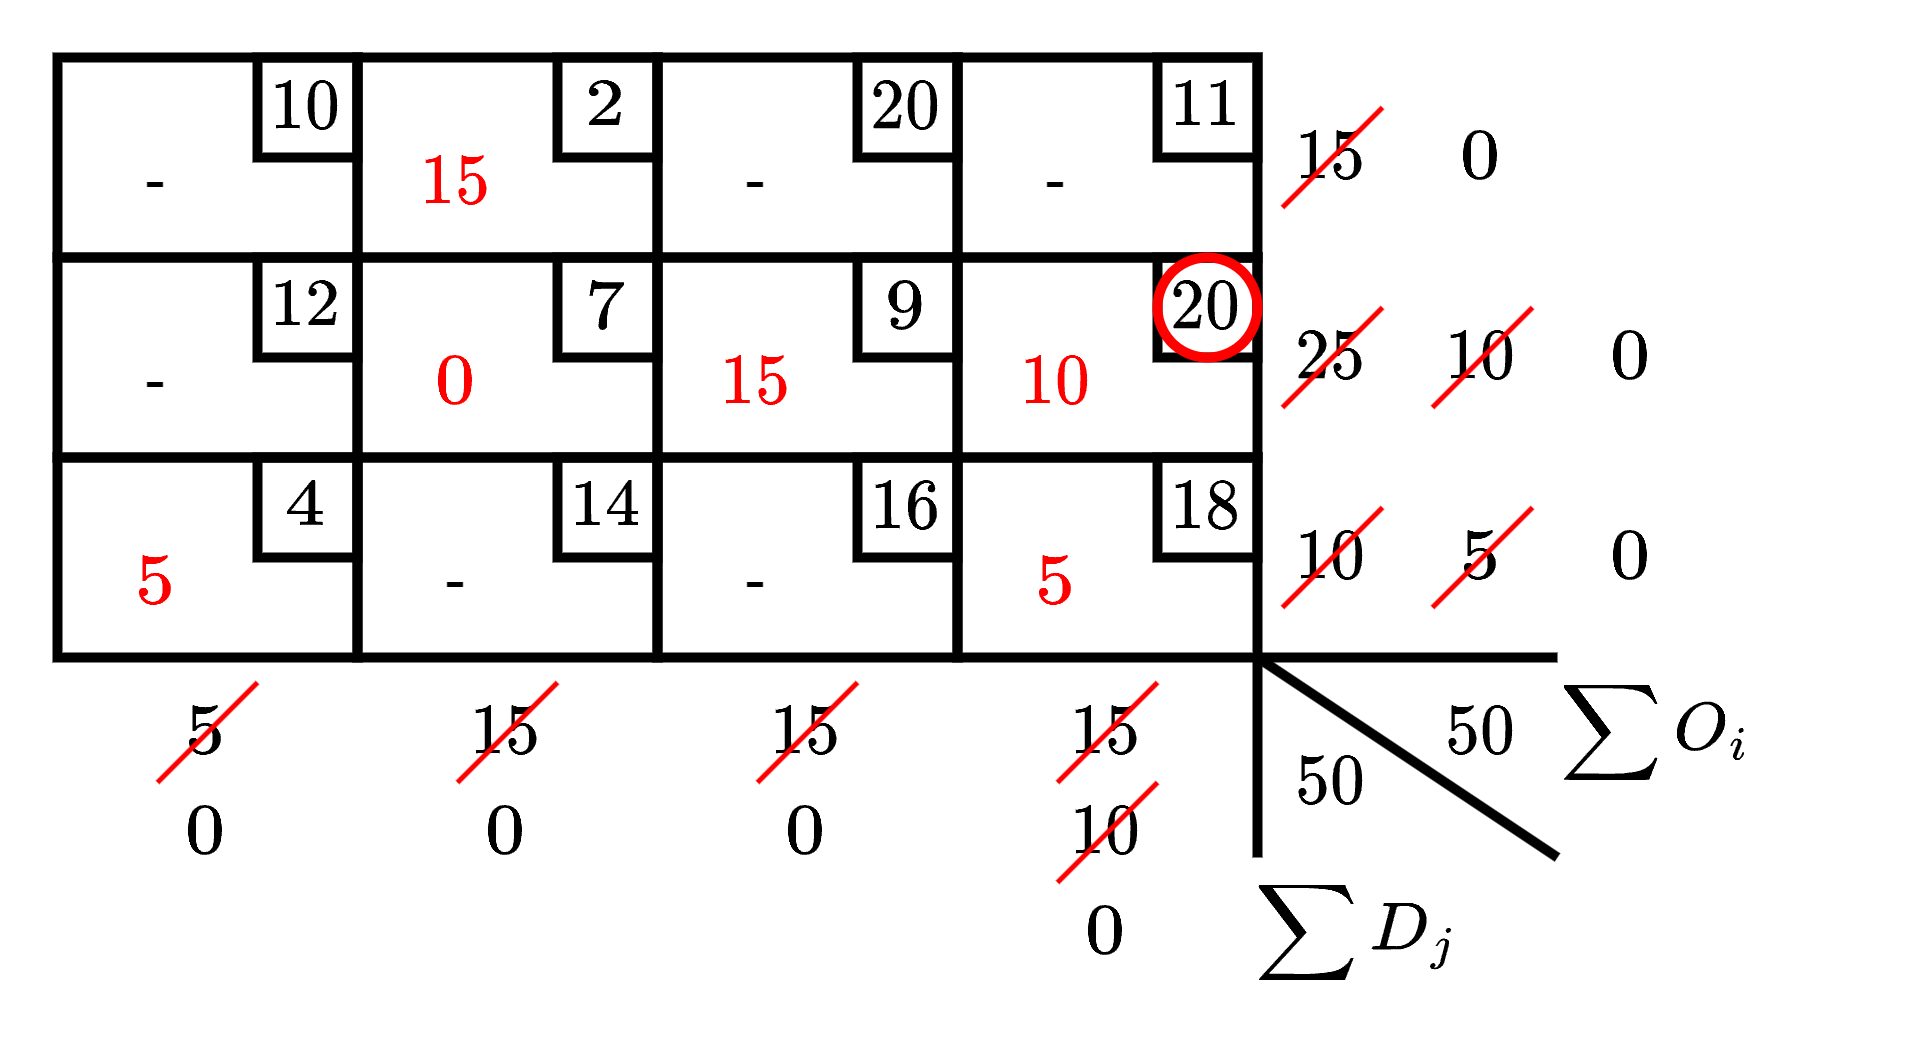
\includegraphics[scale=0.15]{diagram/PTE2CM6.png}
    \end{figure}

    \item Luego se verifica la cantidad de soluciónes factibles.
    \begin{equation*}
        \text{S.F.} = m+n-1 = 6
    \end{equation*}

    \item Para finalizar se calcula el valor de la función objetivo.
    \begin{align*}
        Z &= 15 \cdot 2 + 0 \cdot 7 + 15 \cdot 9 + 10 \cdot 20 + 5 \cdot 4 + 5 \cdot 18\\
        &= 30 + 0 + 135 + 200 + 20 + 90 \\
        &= 475
    \end{align*}
\end{itemize}

\newpage
\subsubsection*{Por Vogël}
Algoritmo:
\begin{itemize}
    \item Se calculan las diferencias de costo entre las celdas con un coste más pequeño, de cada fila y columna, para elegir la mayor diferencia de costo \textit{(penalización)}.
    \begin{figure}[H]
        \centering
        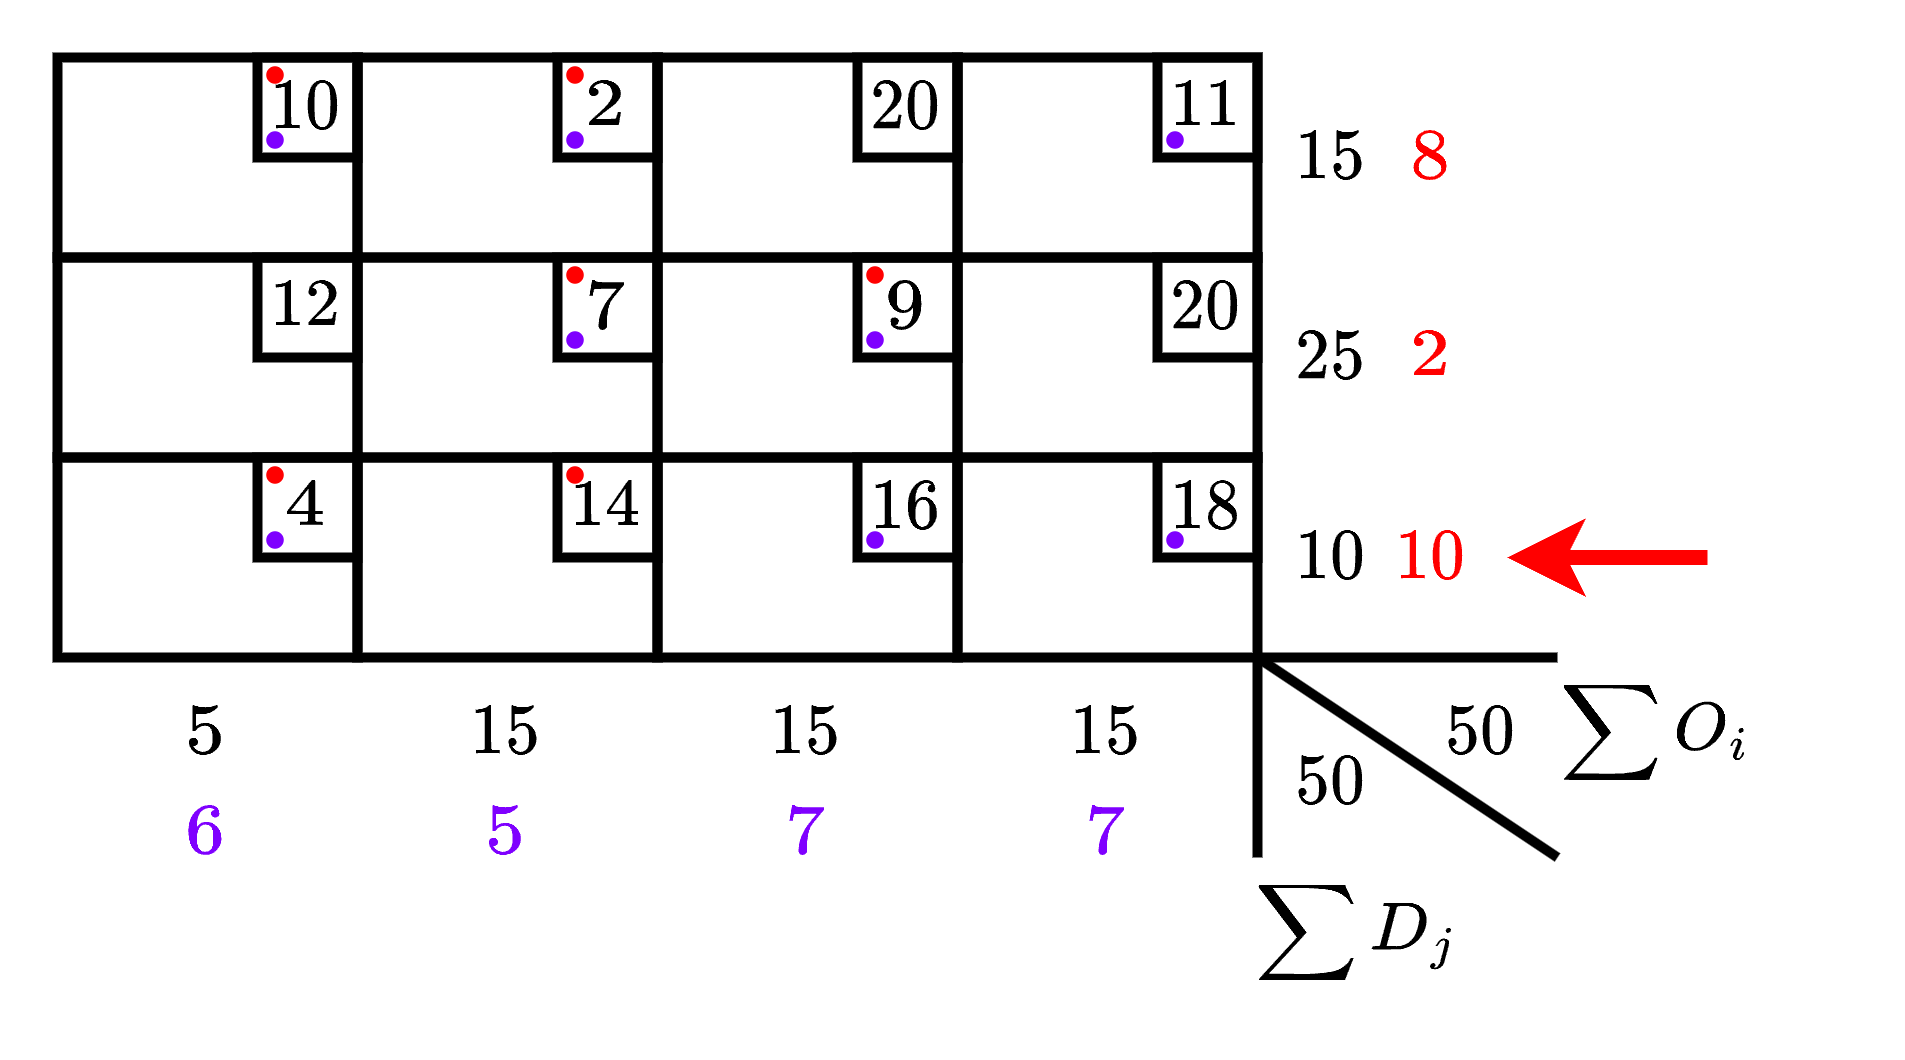
\includegraphics[scale=0.15]{diagram/PTE2V1.png}
    \end{figure}

    \item Se elige la celda con menor $c_{ij}$ de la fila o columna con mayor \textit{penalización}, para asignarle el valor maximo posible de oferta y demanda, luego se elige la fila o columna a rellenar con - de los demas $X_{ij}$.
    \begin{figure}[H]
        \centering
        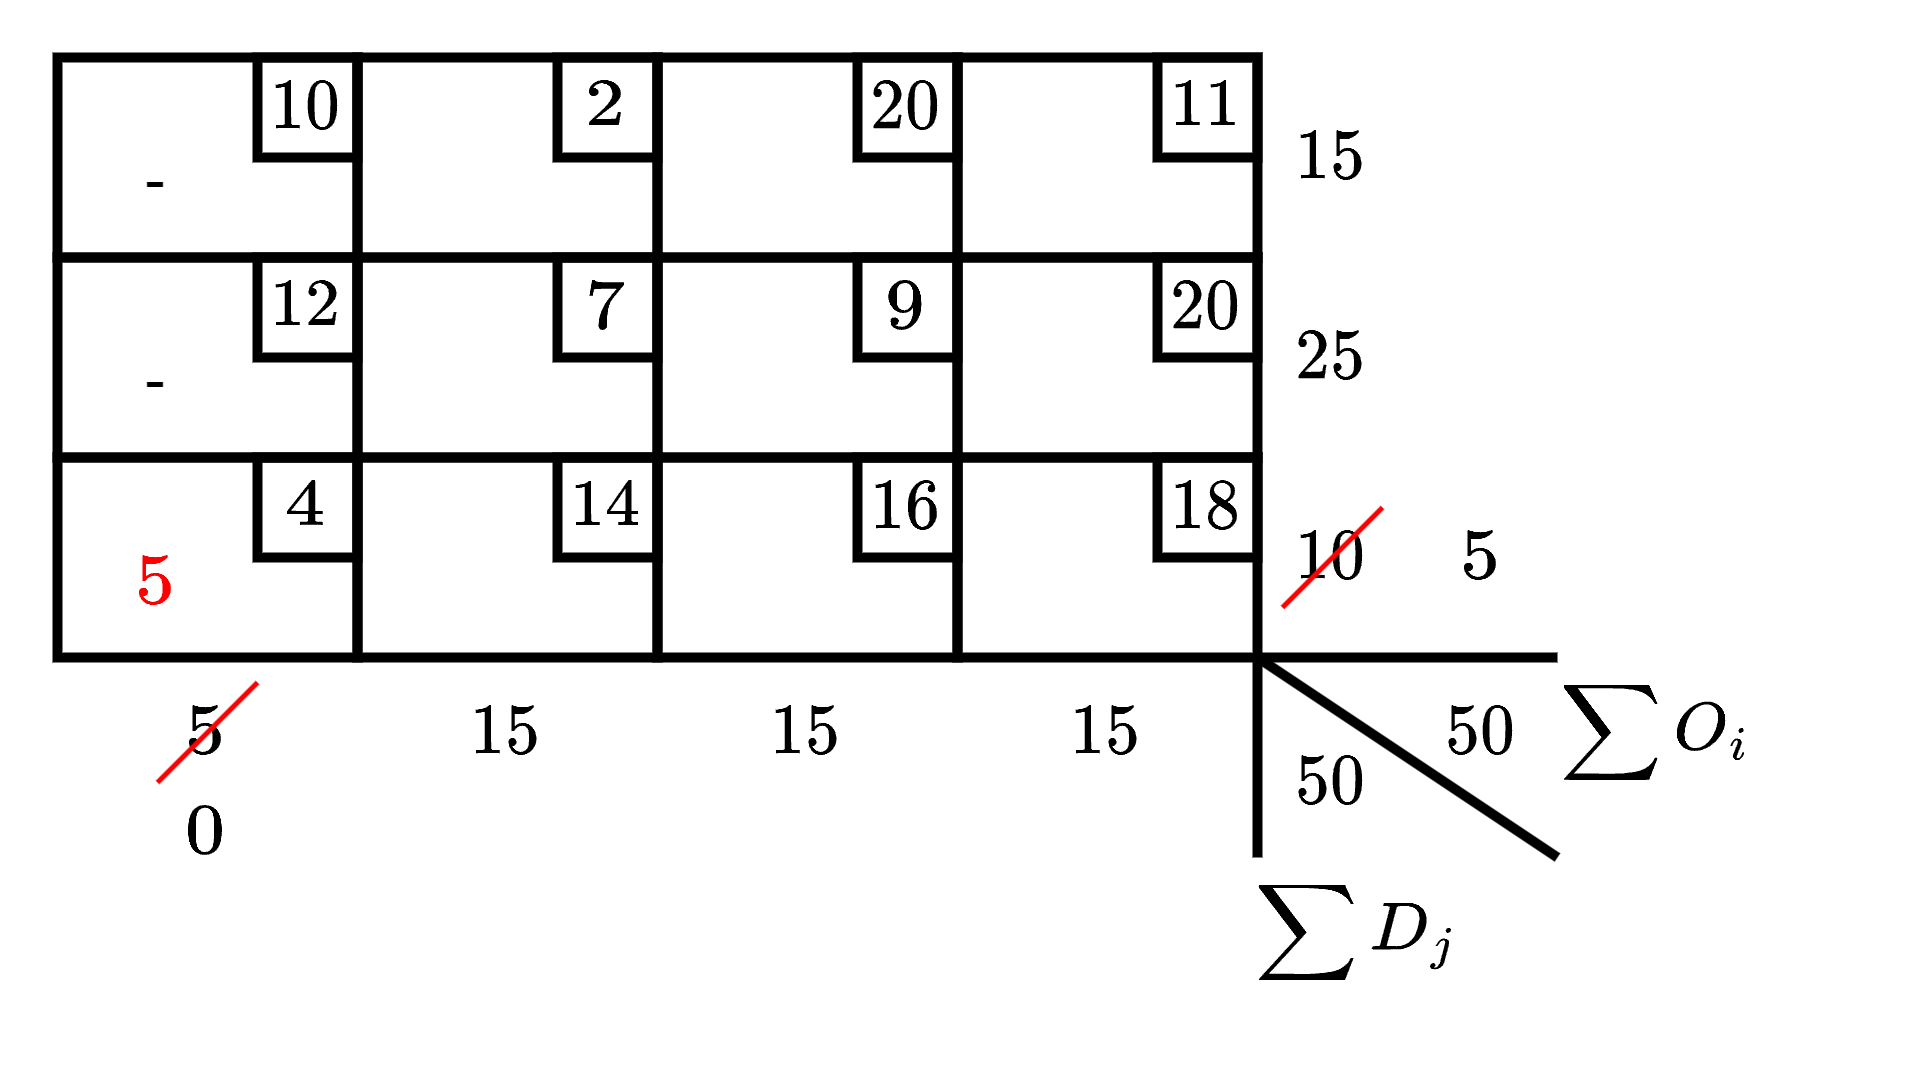
\includegraphics[scale=0.15]{diagram/PTE2V2.png}
    \end{figure}

    \item Se repite el proceso (La fila/columna con - no se utiliza para calcular la \textit{penalización}).
    \begin{figure}[H]
        \centering
        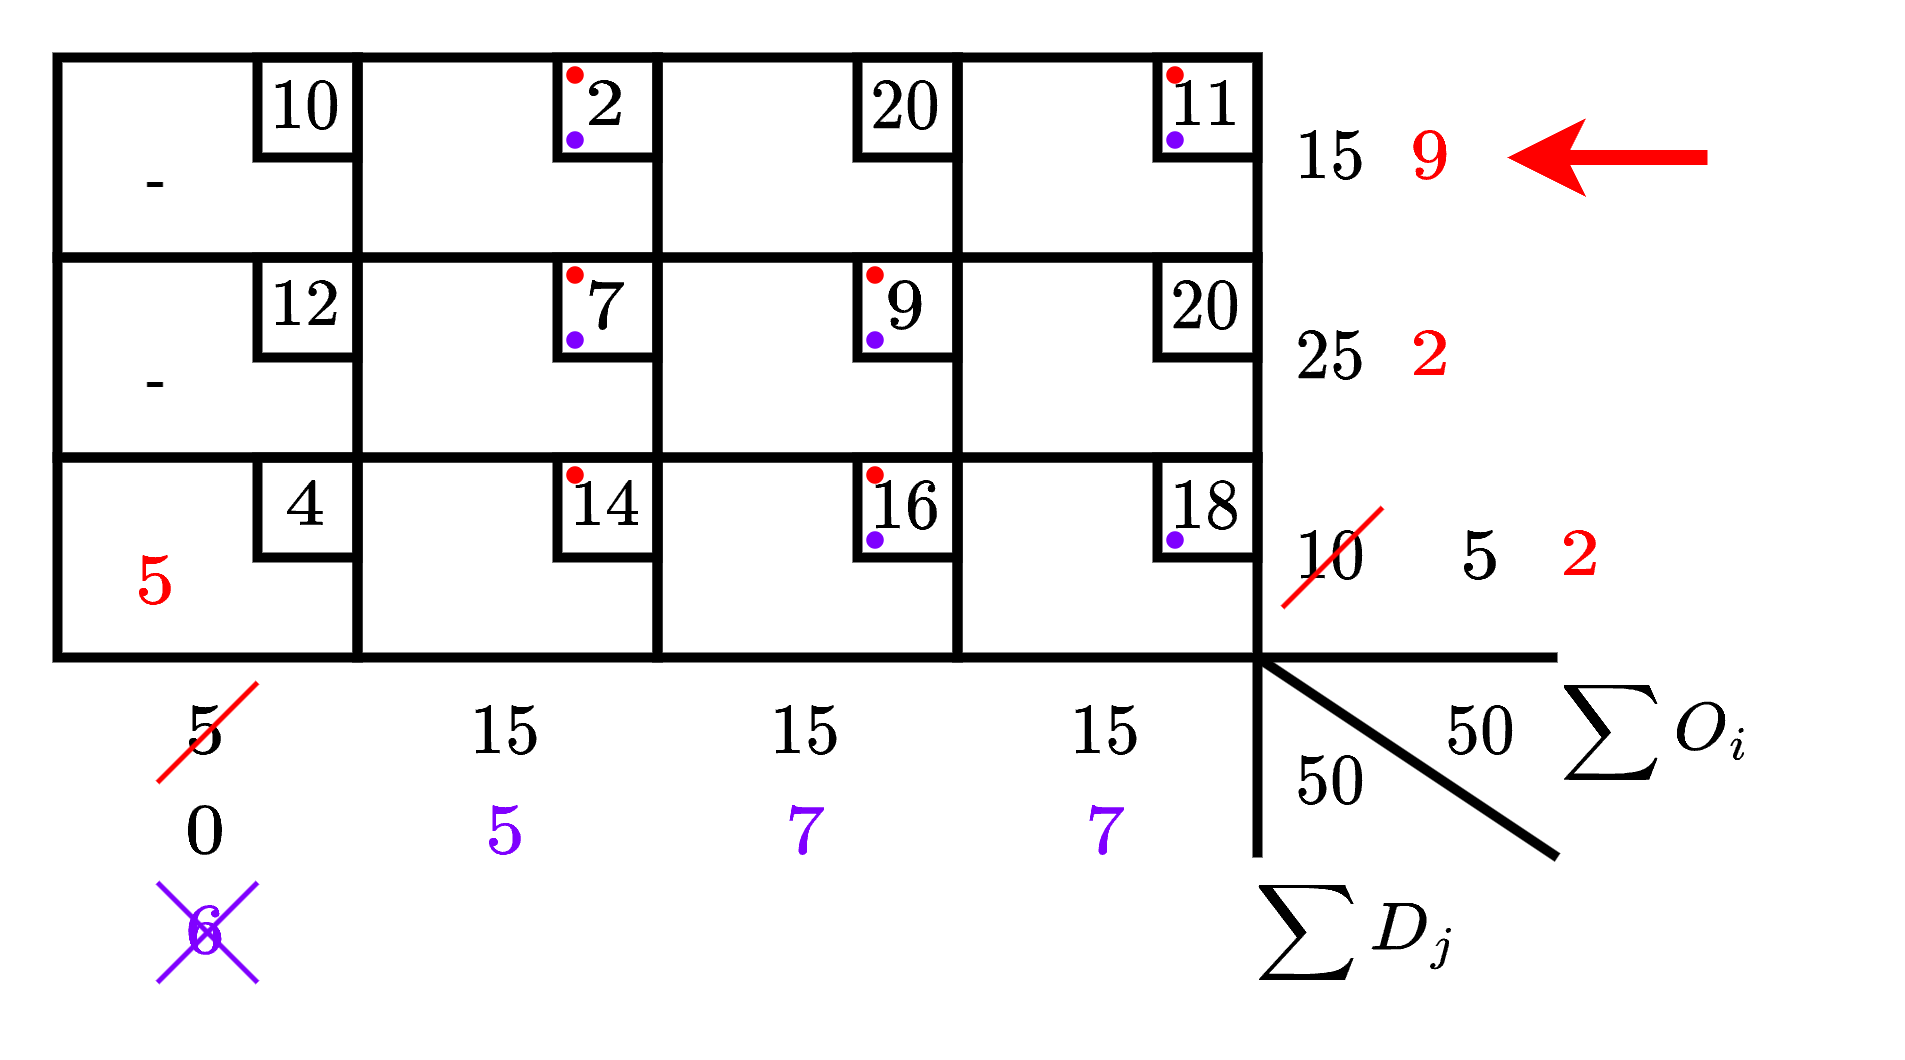
\includegraphics[scale=0.15]{diagram/PTE2V3.png}
    \end{figure}

    \begin{figure}[H]
        \centering
        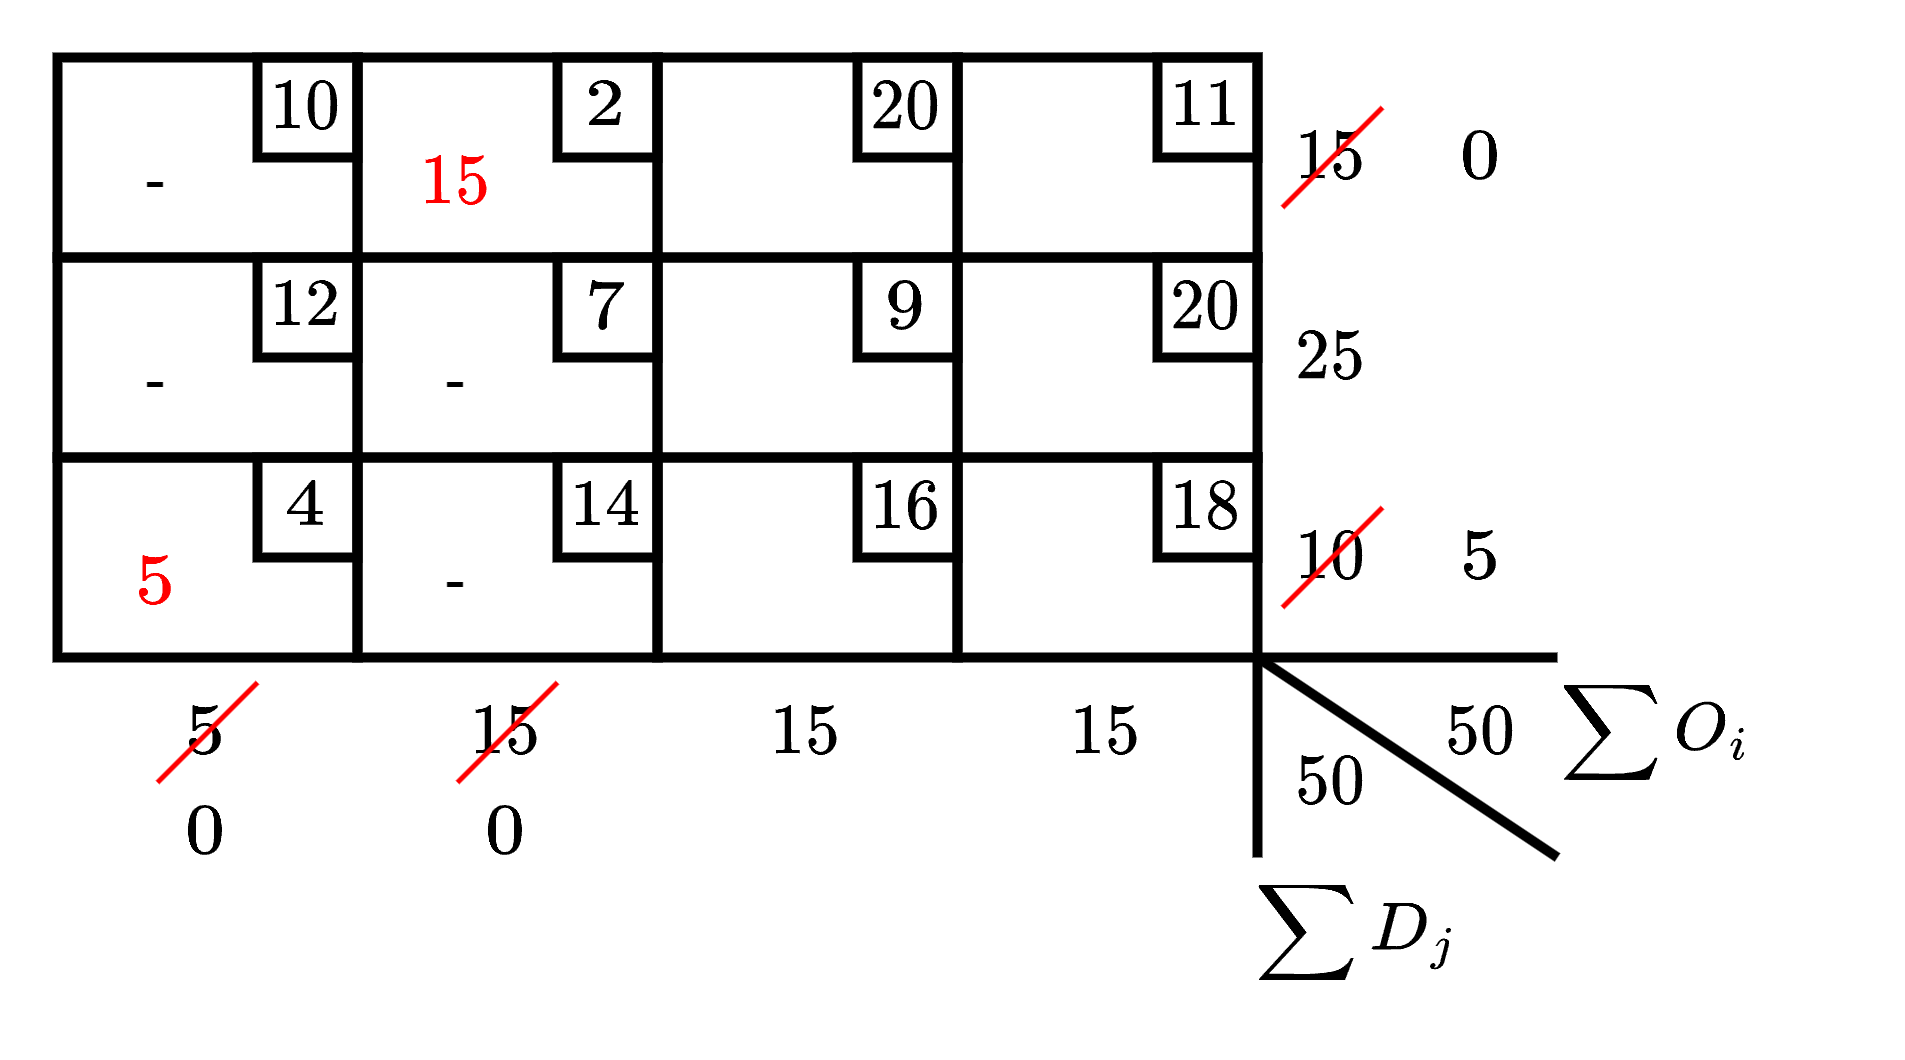
\includegraphics[scale=0.15]{diagram/PTE2V4.png}
    \end{figure}

    \begin{figure}[H]
        \centering
        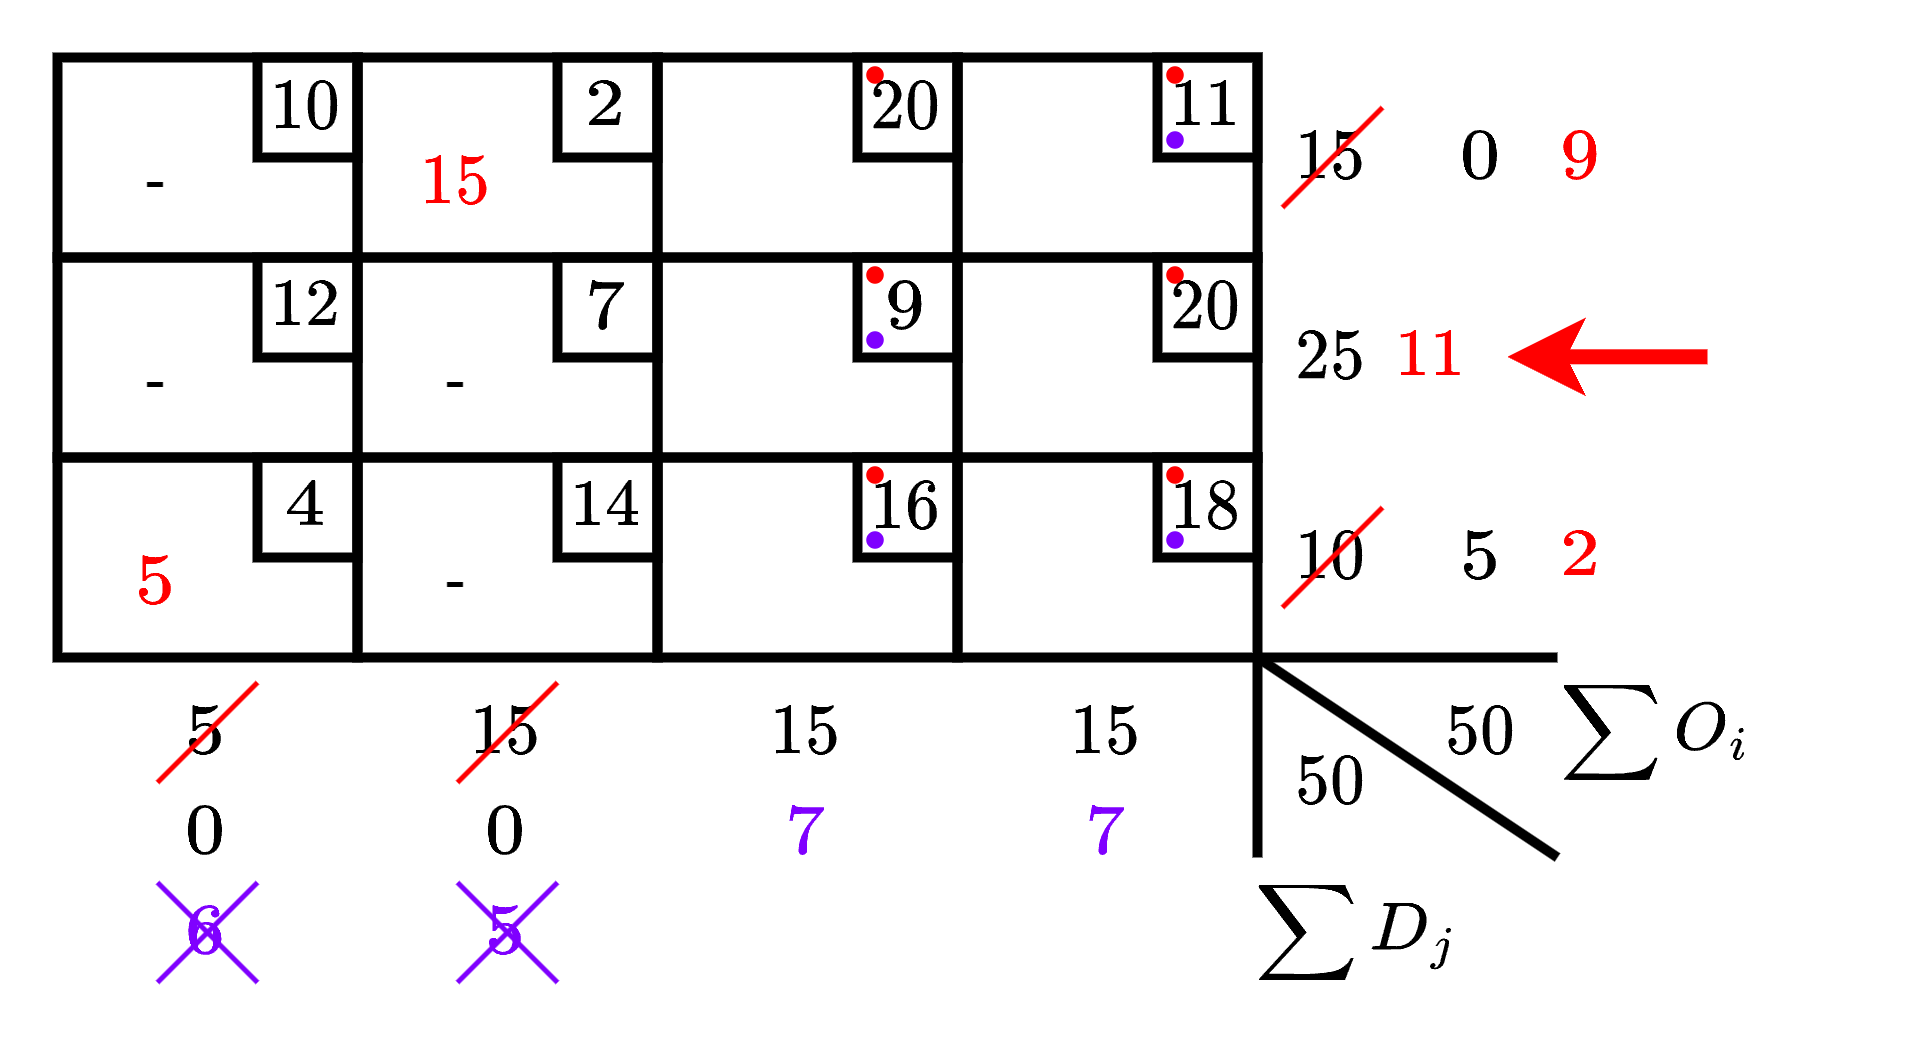
\includegraphics[scale=0.15]{diagram/PTE2V5.png}
    \end{figure}

    \begin{figure}[H]
        \centering
        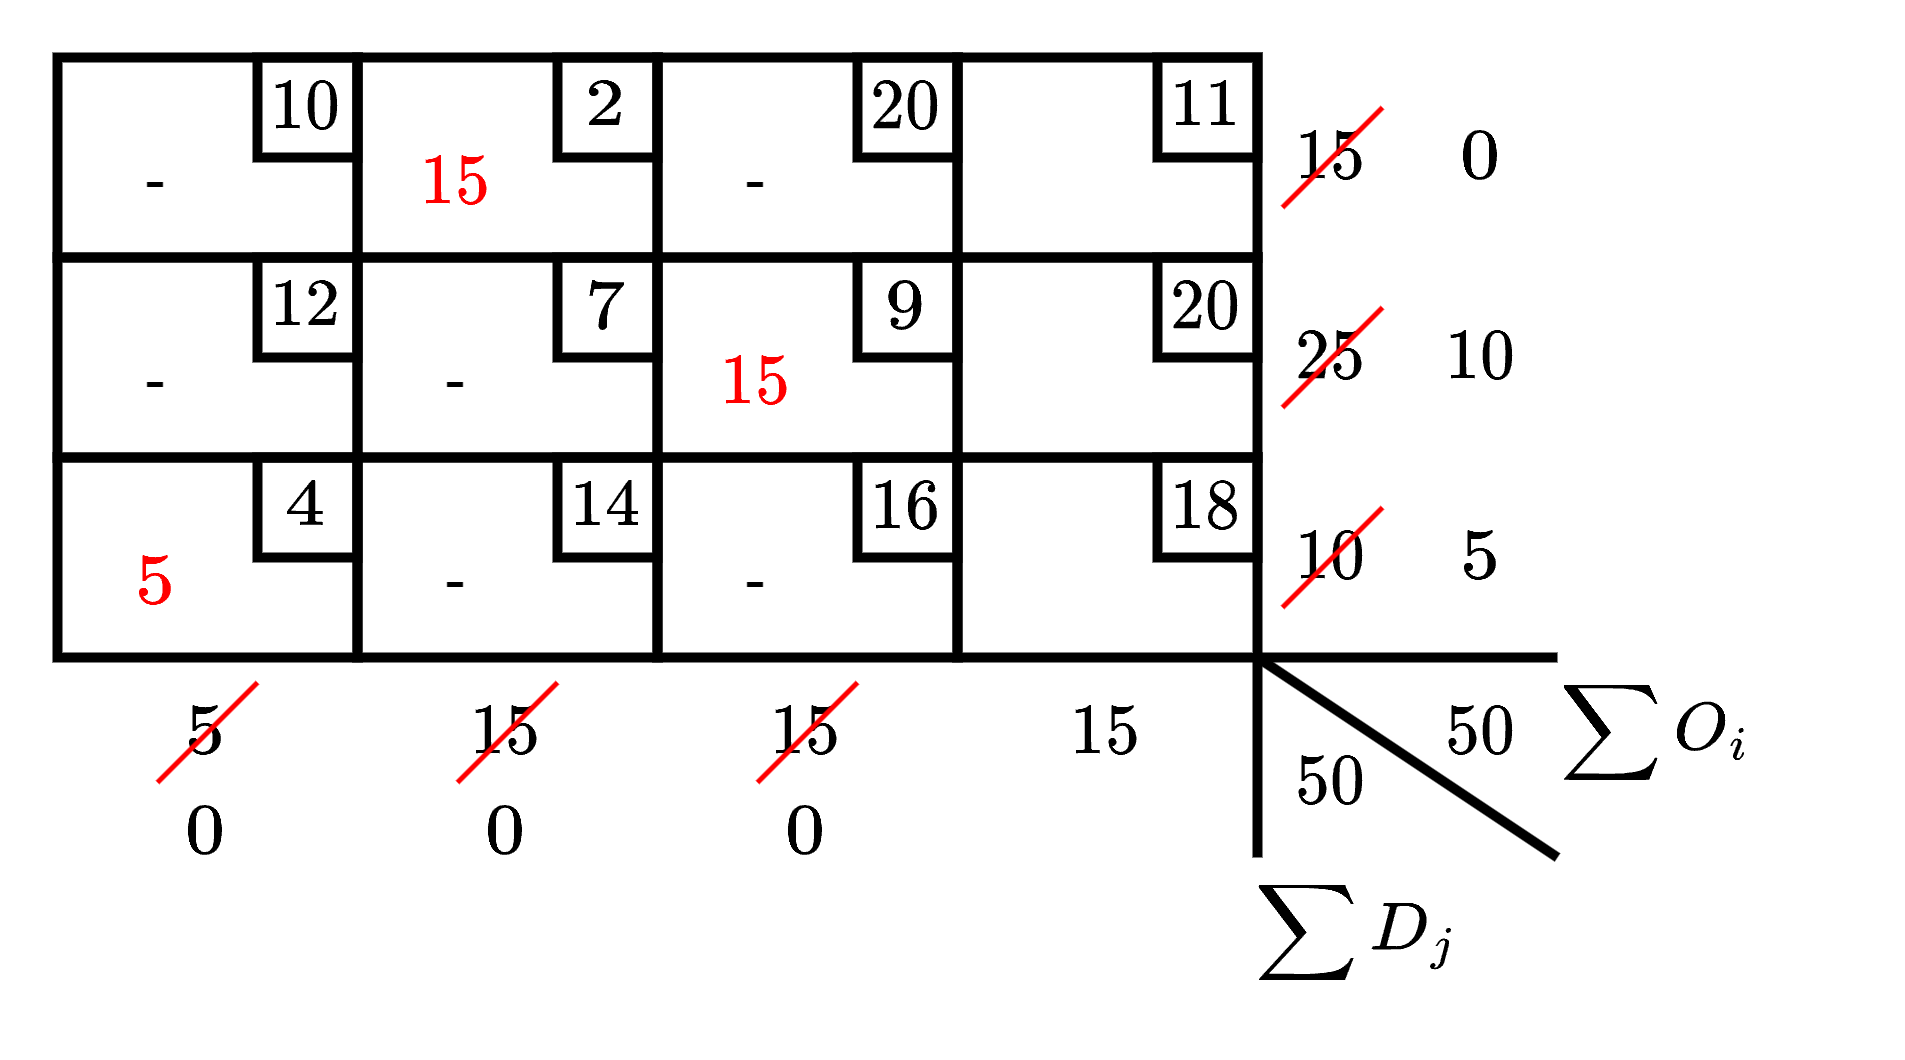
\includegraphics[scale=0.15]{diagram/PTE2V6.png}
    \end{figure}

    \newpage
    \item Al tener las filas o columnas con - se procede a rellenarlas para cumplir con las restricciones y con la cantidad de soluciones factibles.
    \begin{figure}[H]
        \centering
        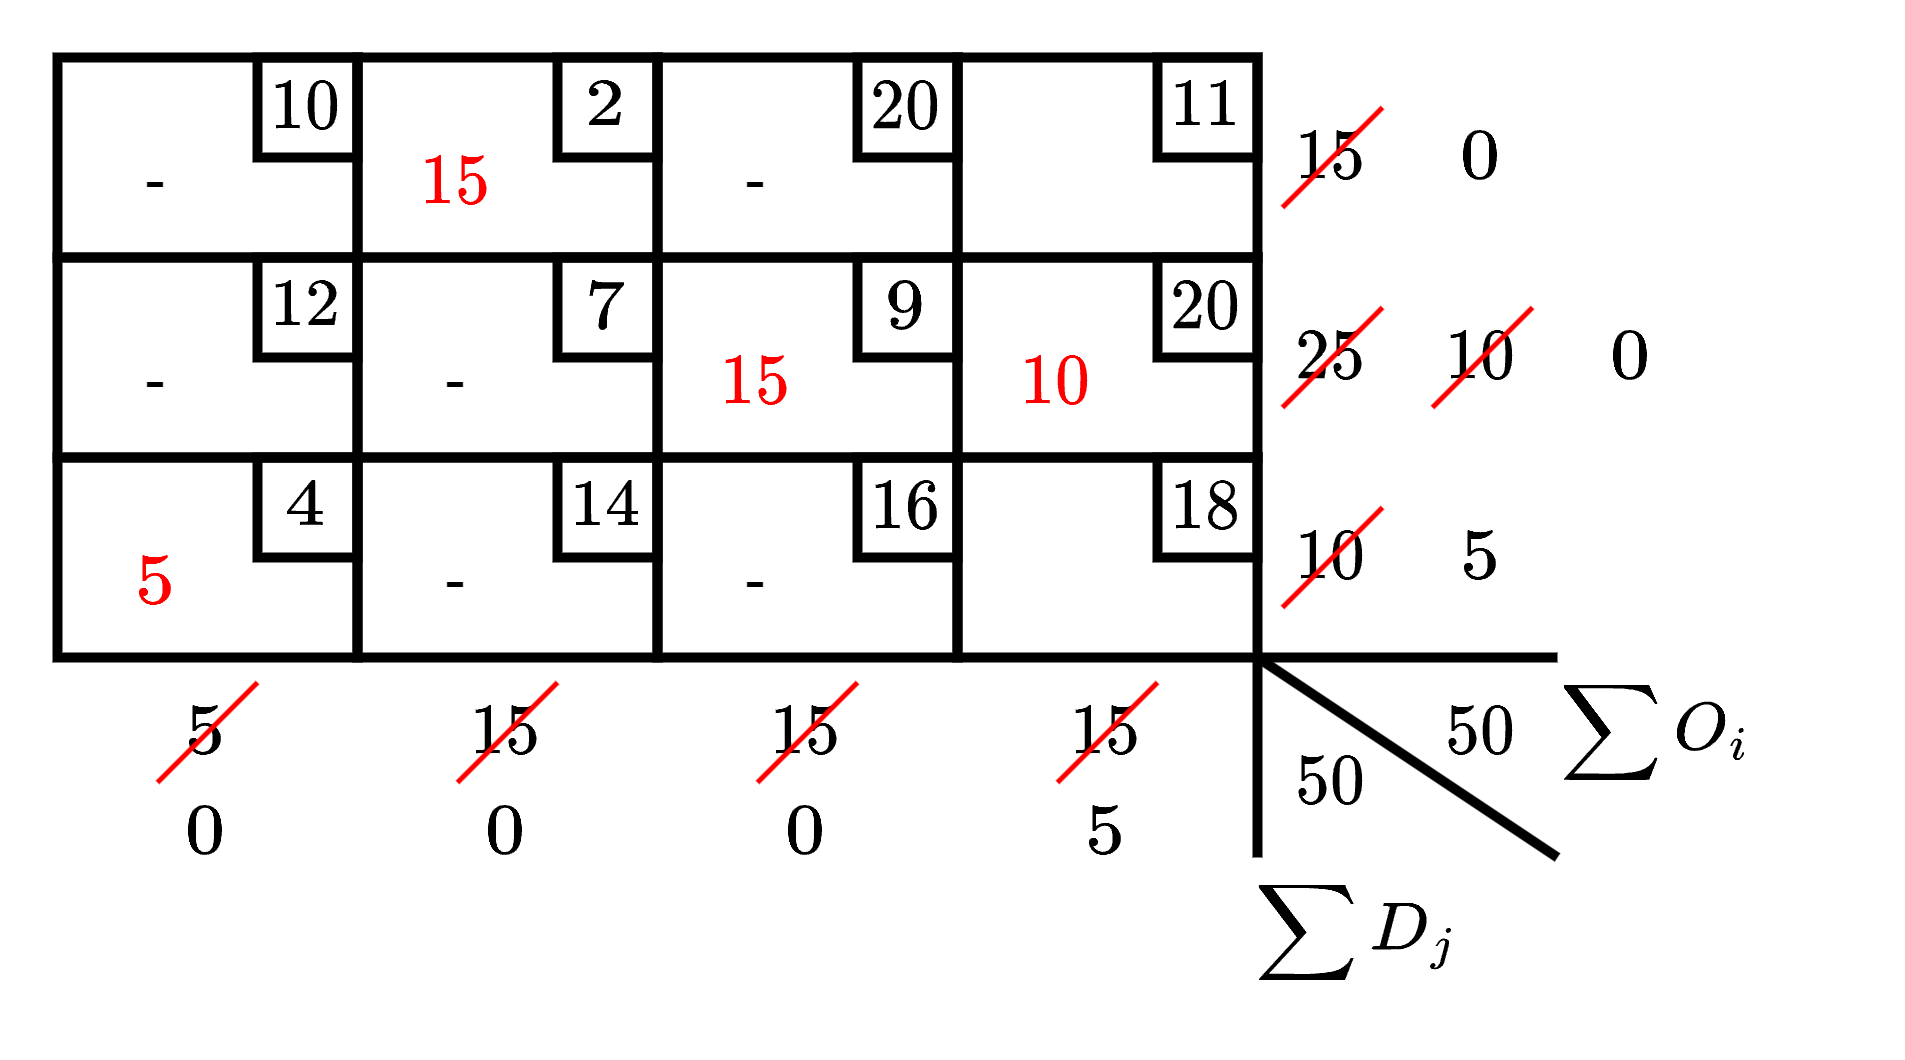
\includegraphics[scale=0.15]{diagram/PTE2V7.png}
    \end{figure}

    \begin{figure}[H]
        \centering
        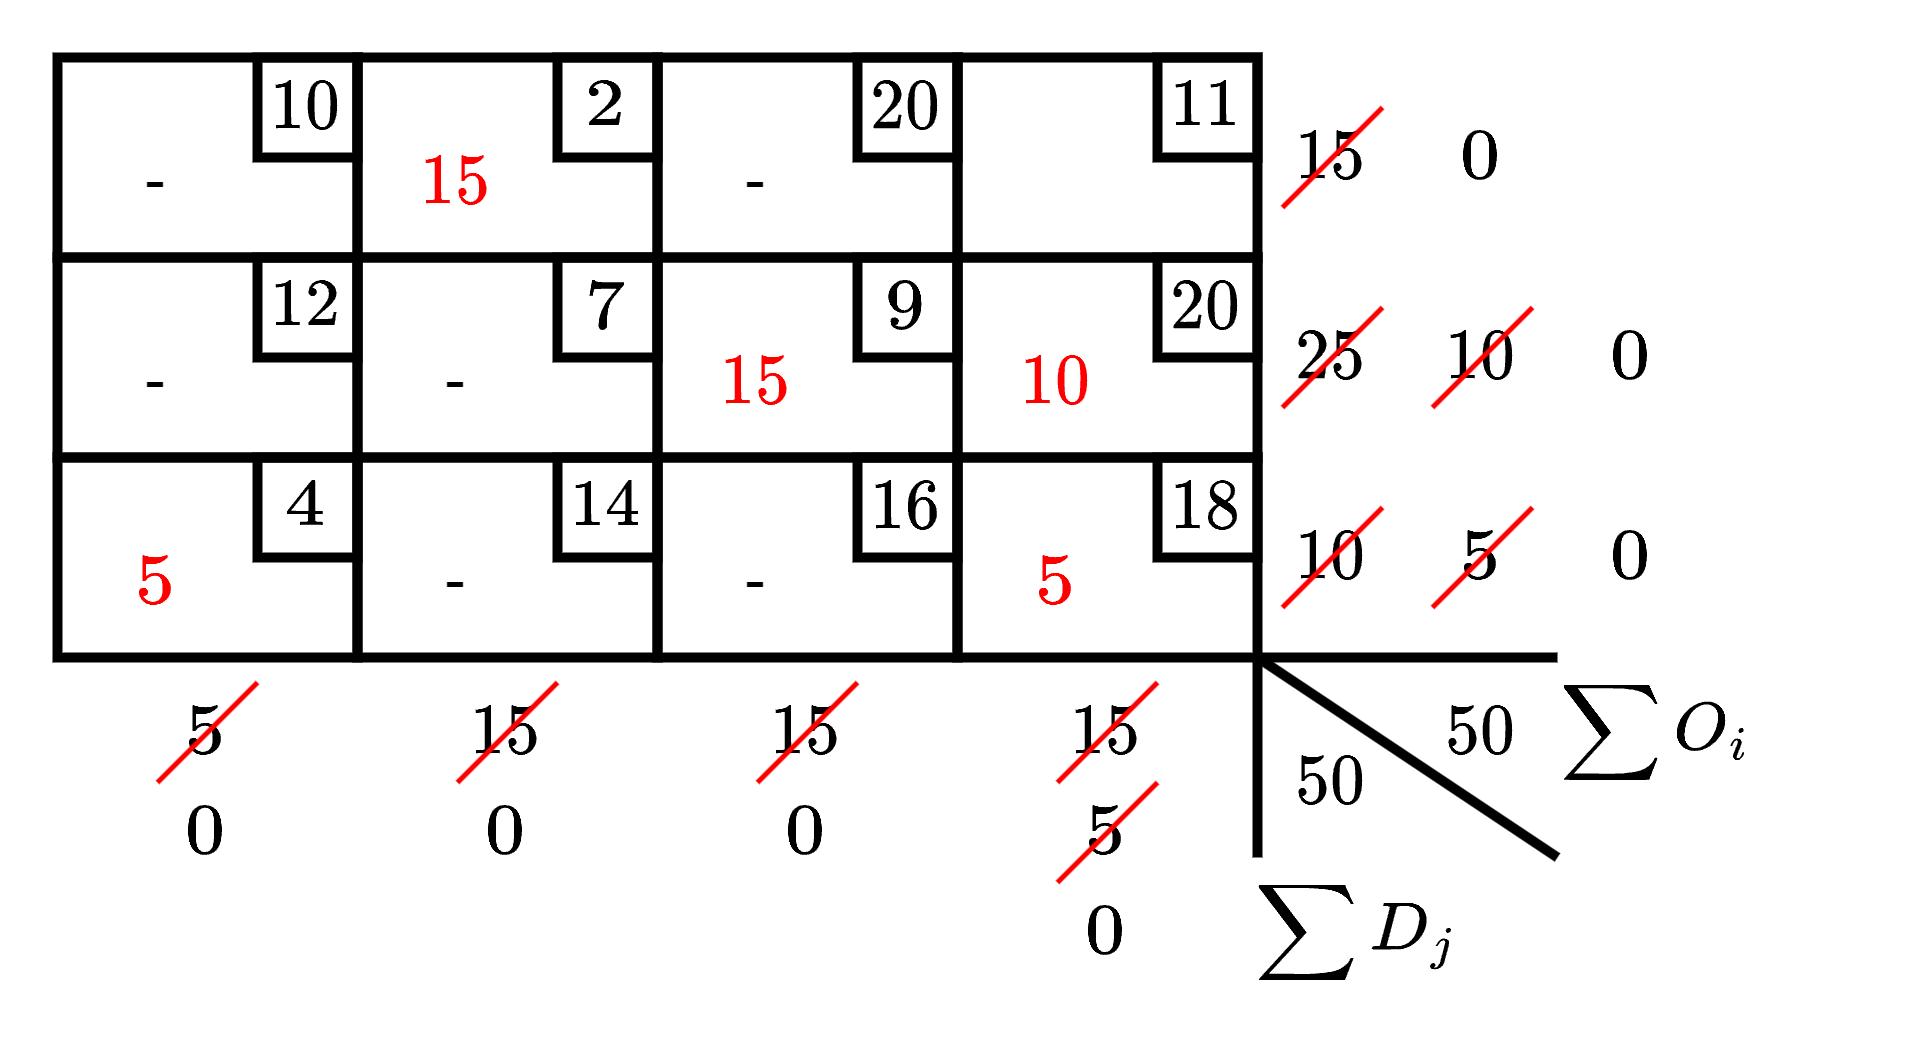
\includegraphics[scale=0.15]{diagram/PTE2V8.png}
    \end{figure}
    
    \begin{figure}[H]
        \centering
        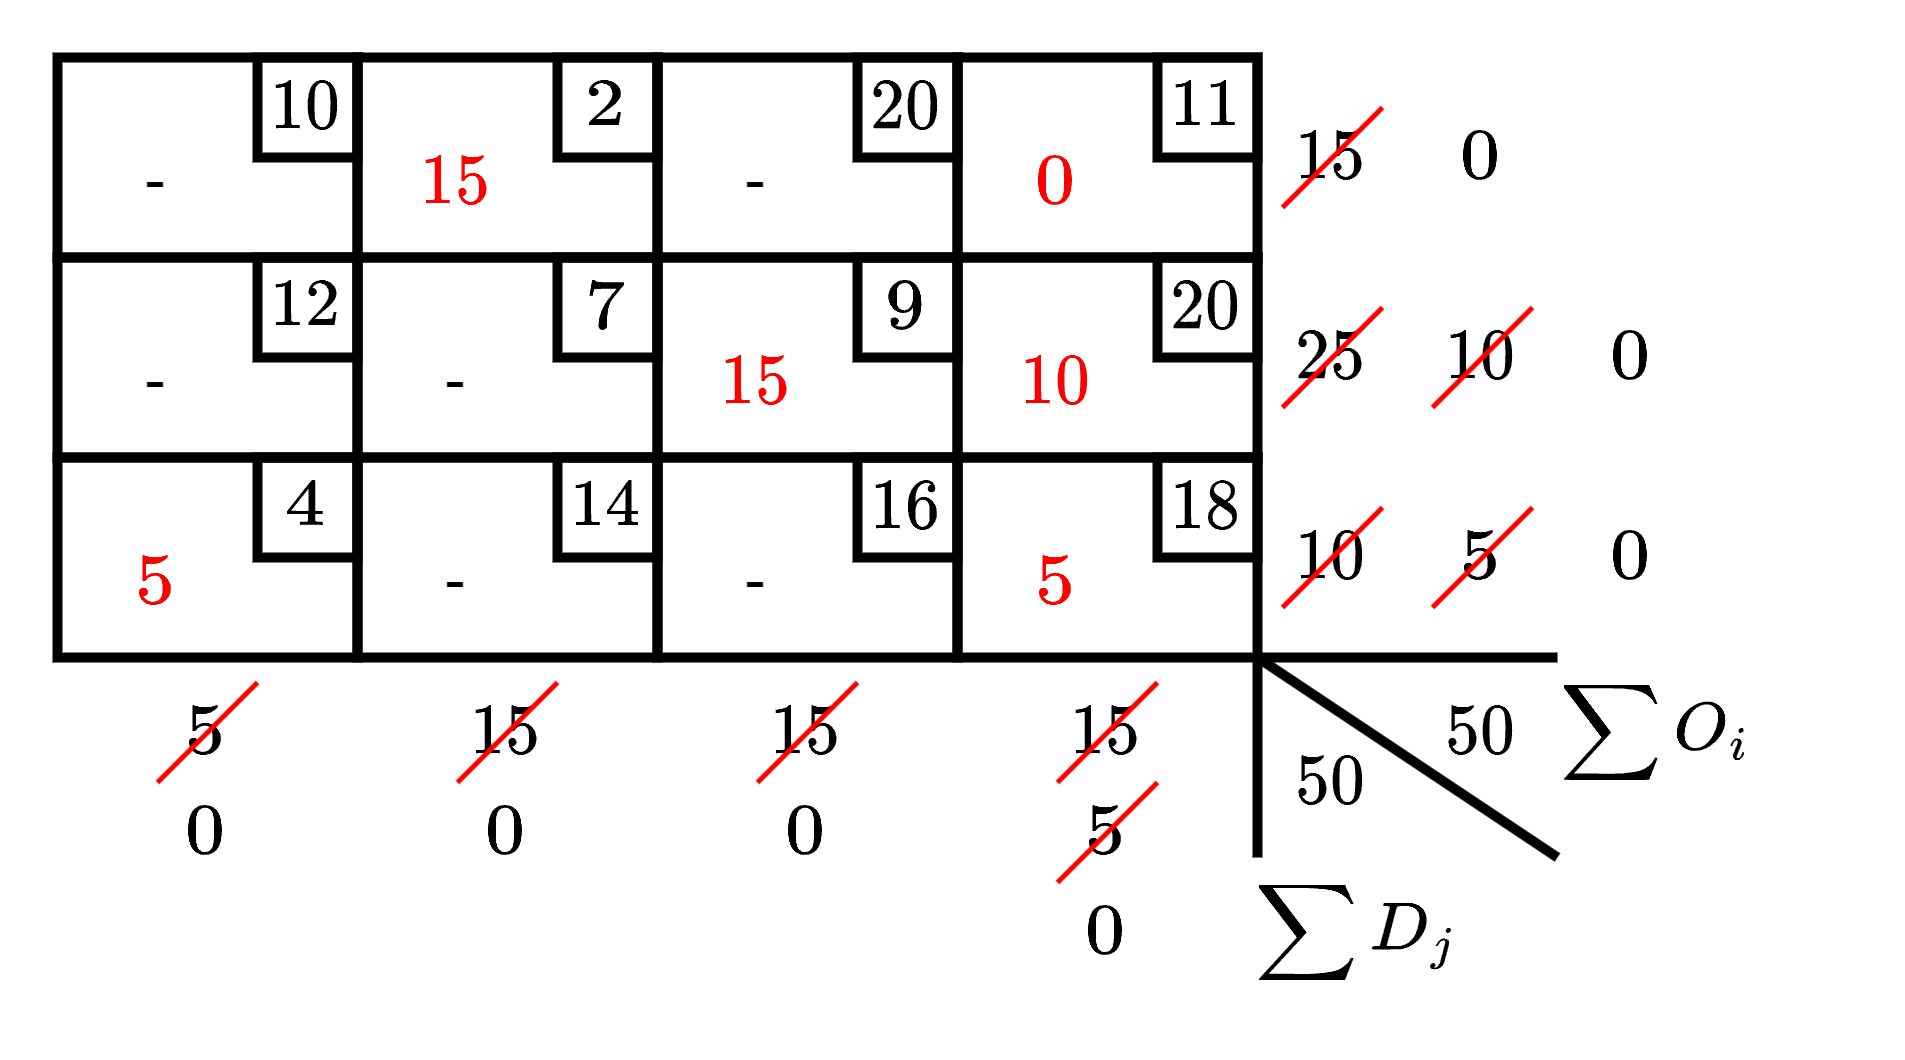
\includegraphics[scale=0.15]{diagram/PTE2V9.png}
    \end{figure}

    \item Se verifica la cantidad de soluciones factibles.
    \begin{equation*}
        \text{S.F.} = m+n-1 = 6
    \end{equation*}

    \item Se calcula el valor de la función objetivo.
    \begin{align*}
        Z &= 15 \cdot 2 + 0 \cdot 11 + 15 \cdot 9 + 10 \cdot 20 + 5 \cdot 4 + 5 \cdot 18\\
        &= 30 + 0 + 135 + 200 + 20 + 90 \\
        &= 475
    \end{align*}
\end{itemize}

\subsubsection*{Para finalizar}
\begin{itemize}
    \item Se comparan los valores de la función objetivo de cada método.
    \begin{align*}
        \text{Regla Nor-Oeste:} \quad Z &= 520 \\
        \text{Costo Mínimo:} \quad Z &= 475 \\
        \text{Vogël:} \quad Z &= 475
    \end{align*}

    \item Se elige el método con el menor valor de la función objetivo.
    \begin{equation*}
        \text{Costo Mínimo y Vogël}
    \end{equation*}
\end{itemize}

\subsection*{Problema 12: Problema de transporte}
Escribir el M.L. para el siguiente P.T.:
\begin{figure}[H]
    \centering
    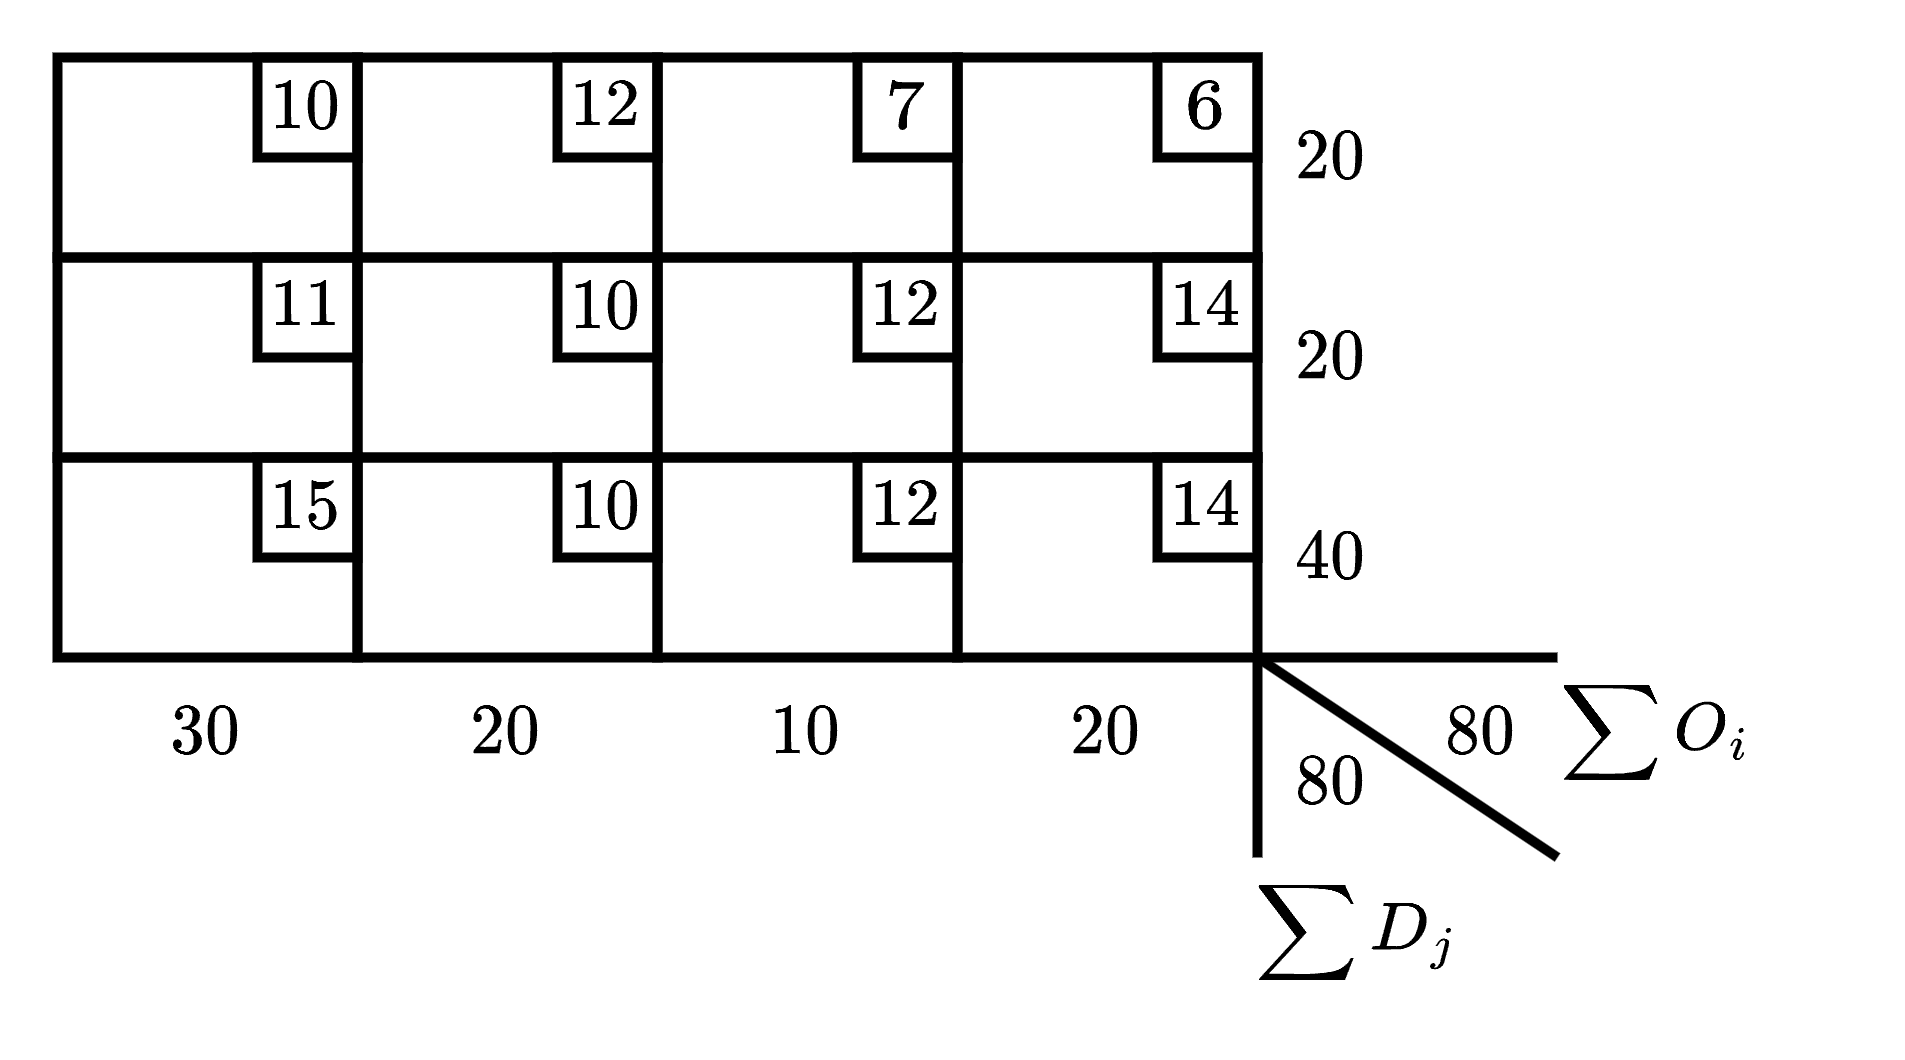
\includegraphics[scale=0.15]{diagram/PTE3.png}
\end{figure}

Donde:
\begin{equation*}
    \text{S.F.} = m+n-1 = 6
\end{equation*}

\newpage
\subsubsection*{Por Regla Nor-Oeste}
\begin{figure}[H]
    \centering
    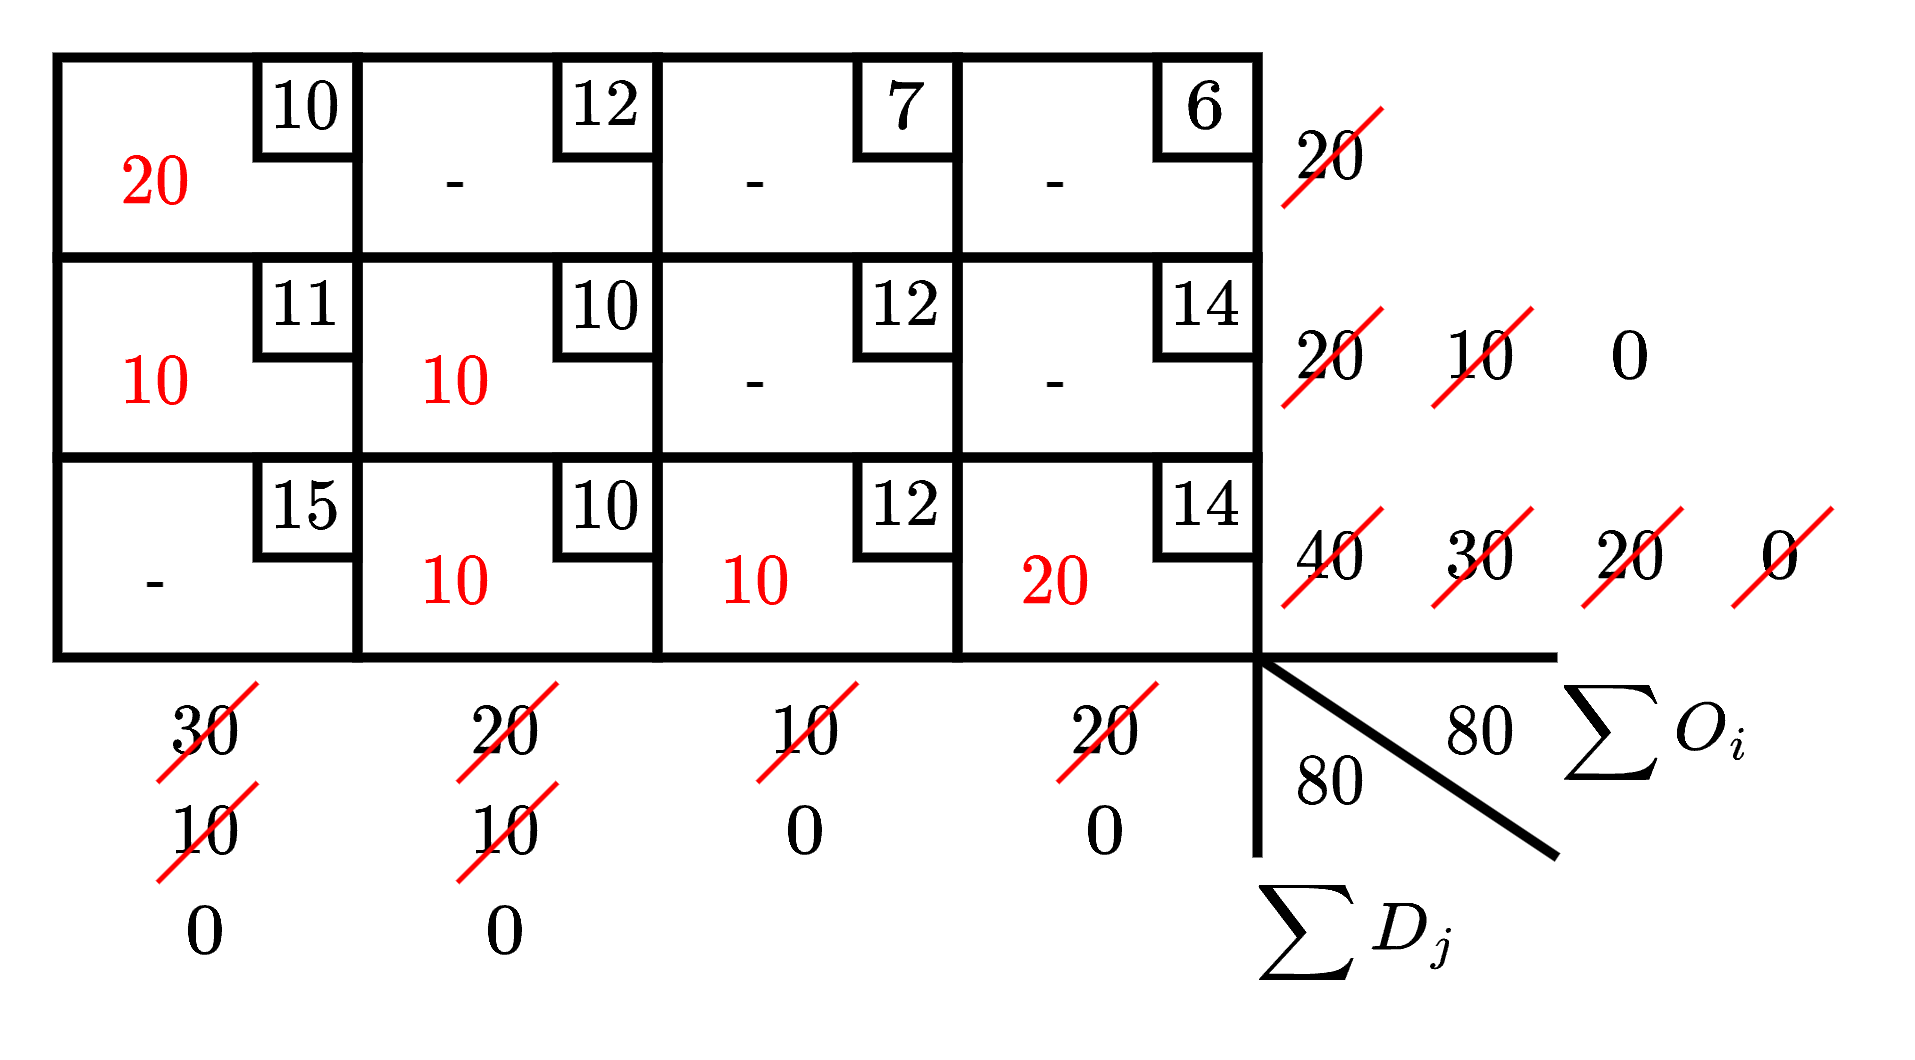
\includegraphics[scale=0.15]{diagram/PTE3RNO.png}
\end{figure}
Valor de la función objetivo:
\begin{align*}
    Z &= 20 \cdot 10 + 10 \cdot 11 + 10 \cdot 10 + 10 \cdot 10 + 10 \cdot 12 + 20 \cdot 14 \\
    &= 200 + 110 + 100 + 100 + 120 + 280 \\
    &= 910
\end{align*}

\subsubsection*{Por Costo Mínimo}
\begin{figure}[H]
    \centering
    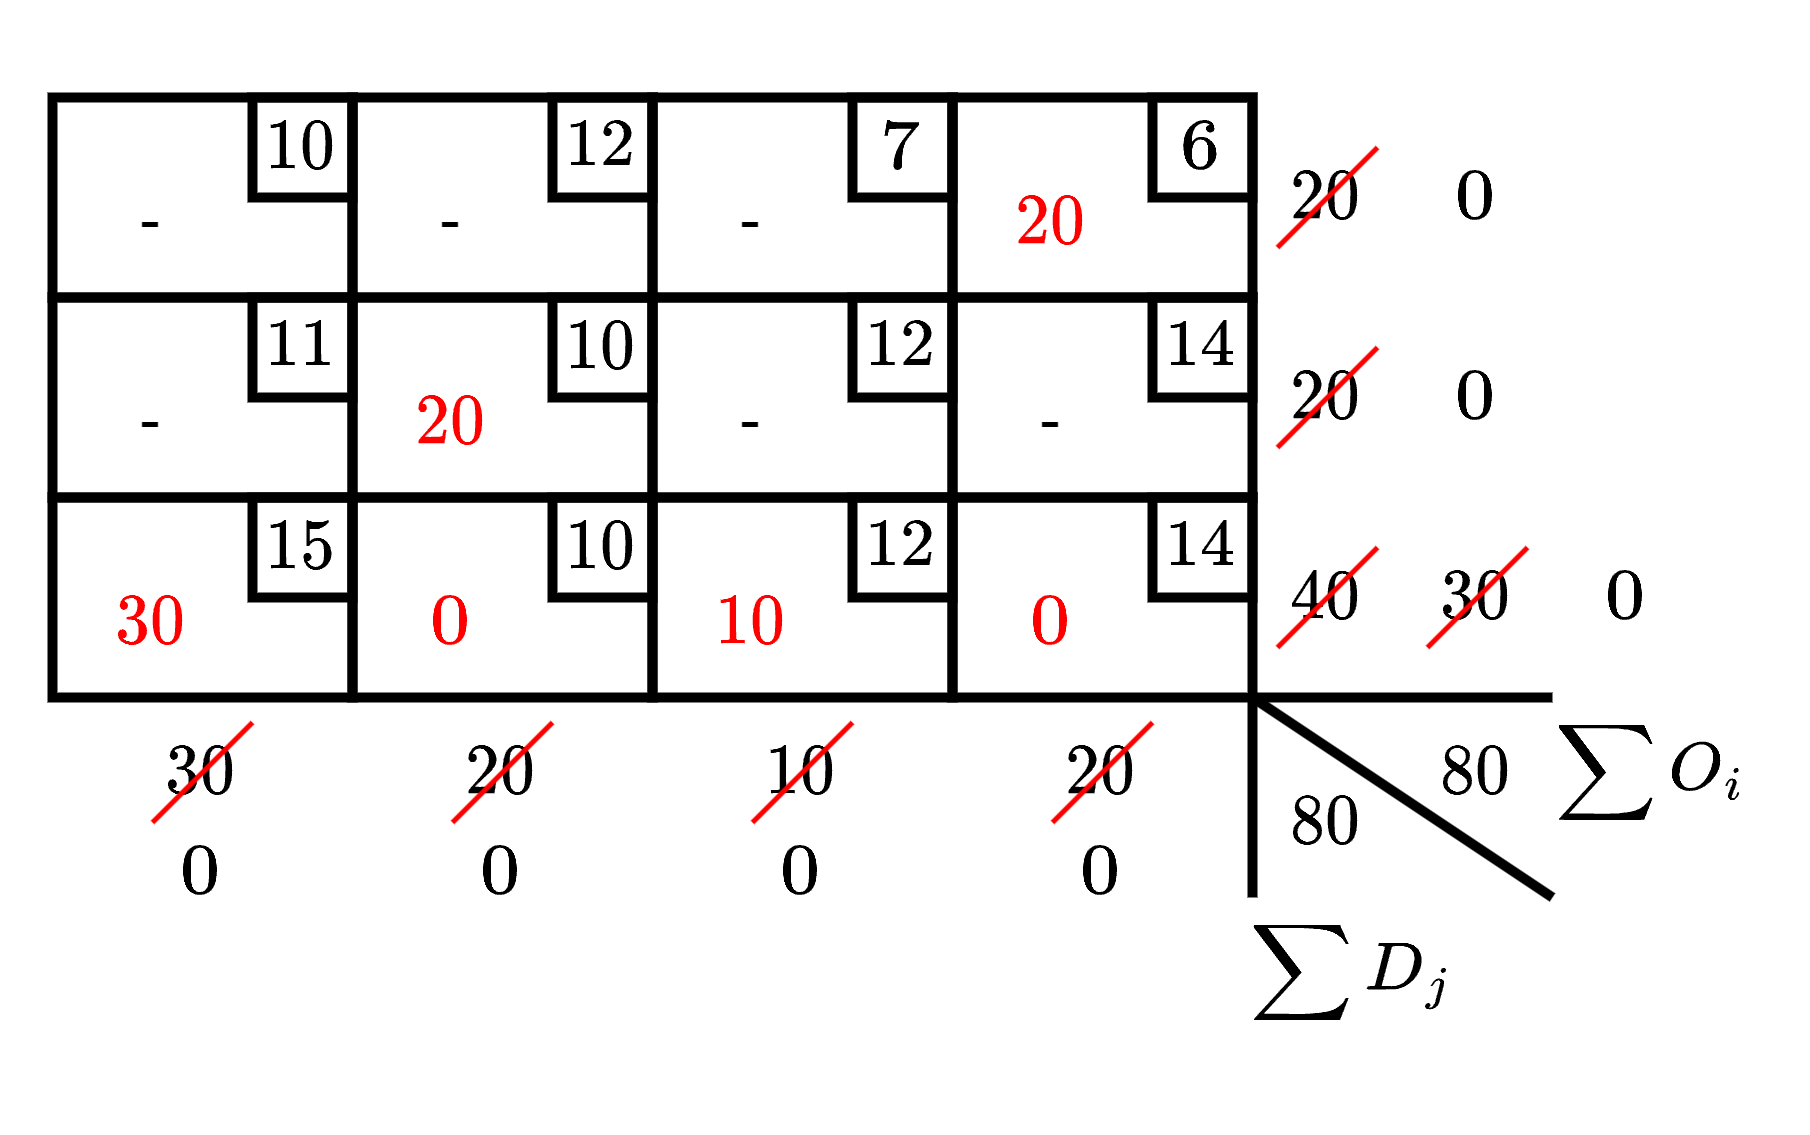
\includegraphics[scale=0.15]{diagram/PTE3CM.png}
\end{figure}
Valor de la función objetivo:
\begin{align*}
    Z &= 20 \cdot 6 + 20 \cdot 10 + 30 \cdot 15 + 0 \cdot 10 + 10 \cdot 12 + 0 \cdot 14 \\
    &= 120 + 200 + 450 + 0 + 120 + 0 \\
    &= 890
\end{align*}

\subsubsection*{Por Vogël}
\begin{figure}[H]
    \centering
    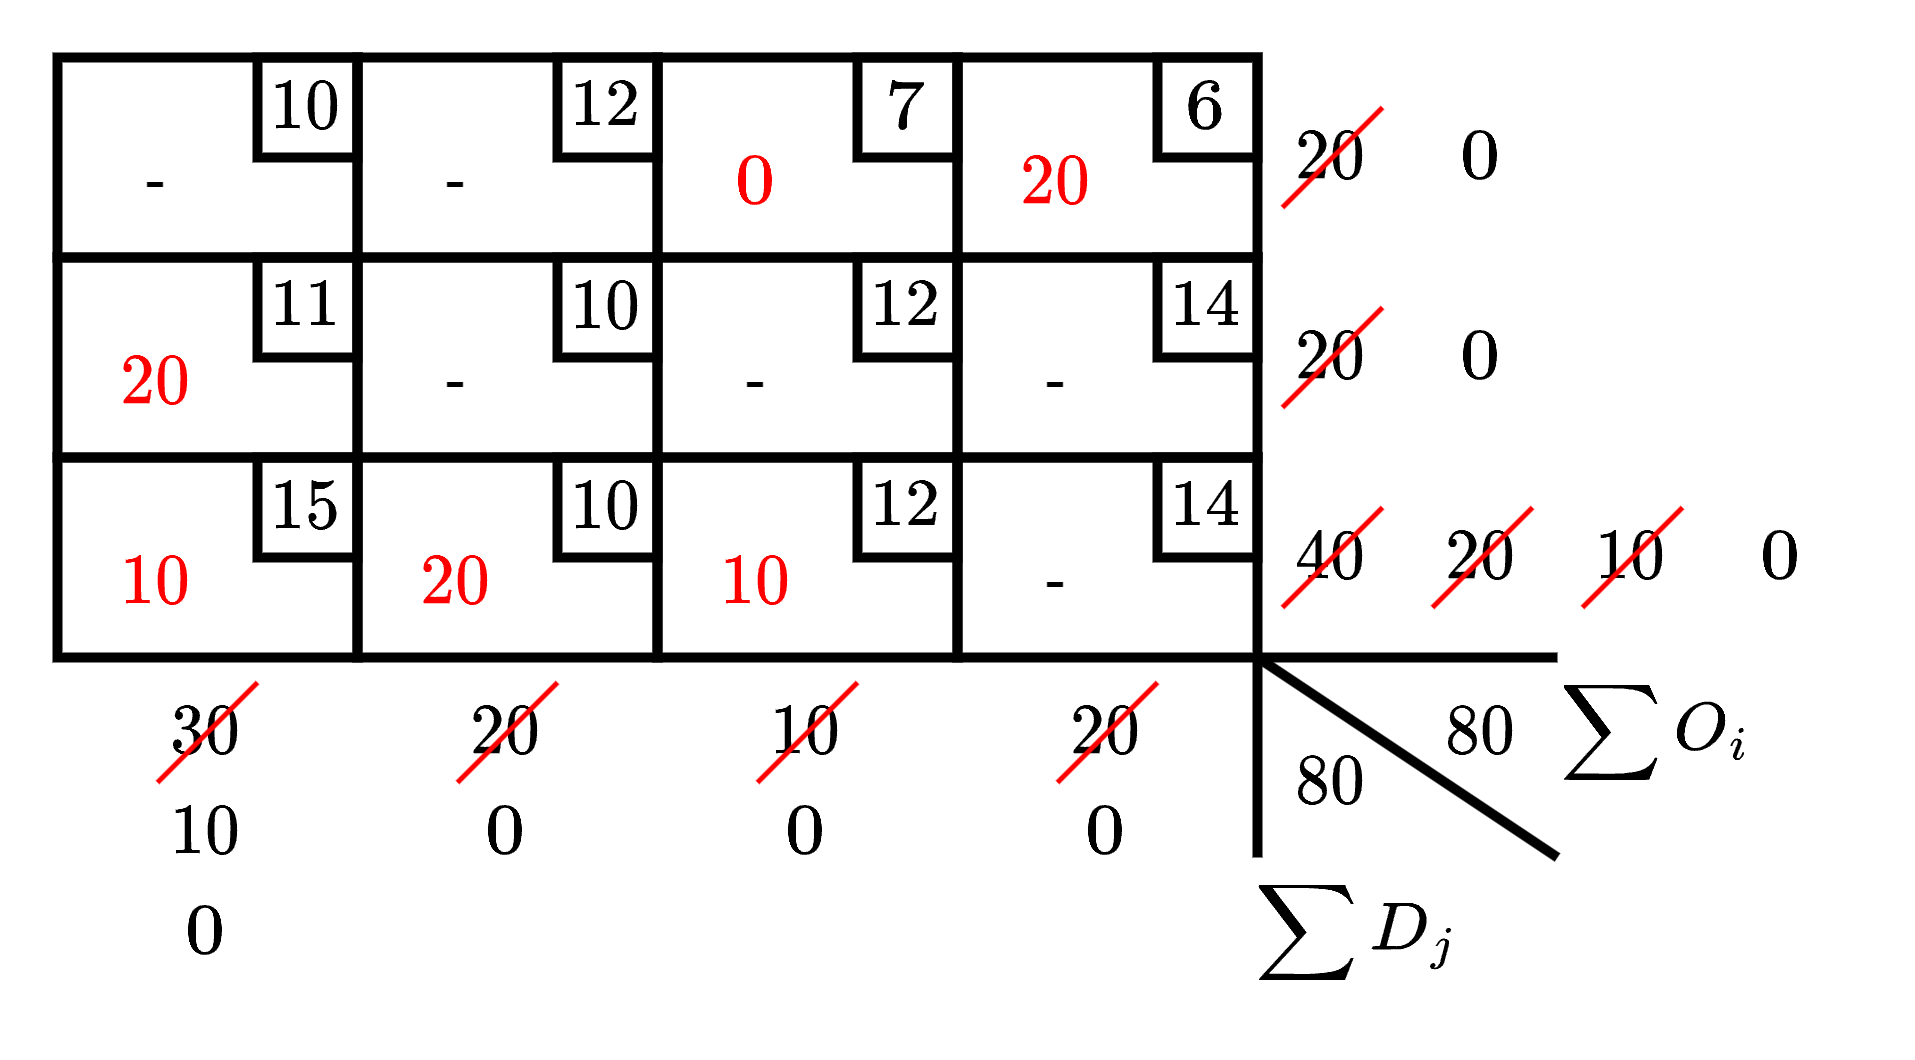
\includegraphics[scale=0.15]{diagram/PTE3V.png}
\end{figure}
Valor de la función objetivo:
\begin{align*}
    Z &= 0 \cdot 7 + 20 \cdot 6 + 20 \cdot 11 + 10 \cdot 15 + 20 \cdot 10 + 10 \cdot 12 \\
    &= 0 + 120 + 220 + 150 + 200 + 120 \\
    &= 810
\end{align*}

\newpage
\subsection*{Problema 13: Relación entre Tabla Simplex Primal y Problema de Transporte [Criterios]}
Sea el siguiente P.T. resuelto por Regla Nor-Oeste:
\begin{figure}[H]
    \centering
    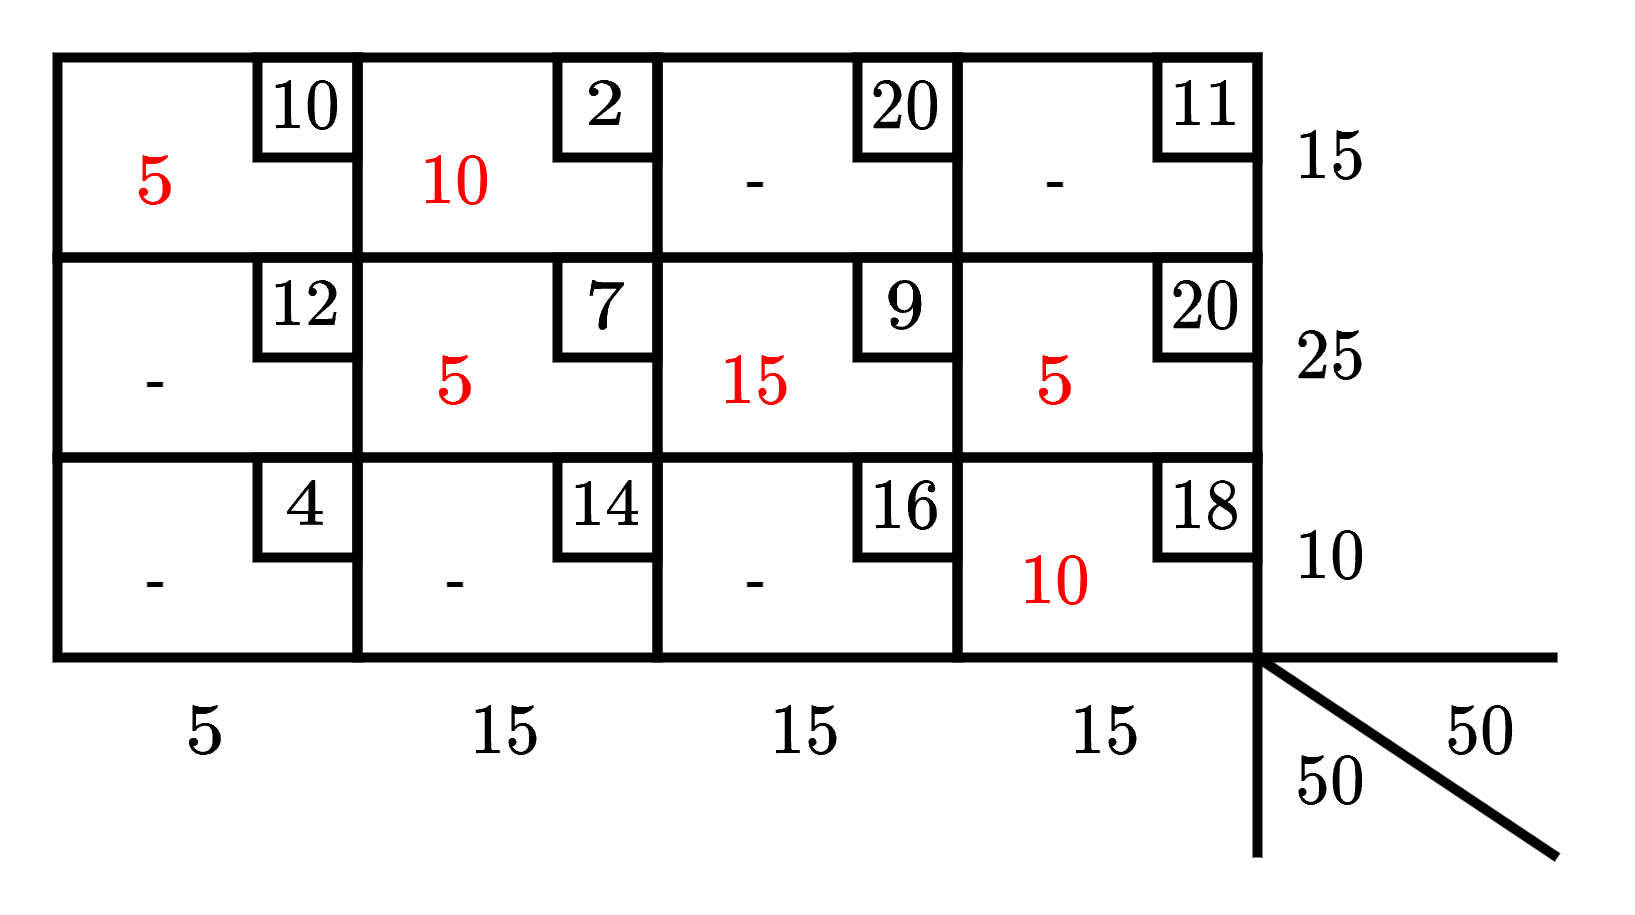
\includegraphics[scale=0.15]{diagram/PTE4.png}
\end{figure}
\begin{align*}
    Z &= 5 \cdot 10 + 10 \cdot 2 + 5 \cdot 7 + 15 \cdot 9 + 5 \cdot 20 + 10 \cdot 18\\
    &= 50 + 20 + 35 + 135 + 100 + 180 \\
    &= 520
\end{align*}
Tabla Simplex Primal:
\begin{center}
    \begin{tabular}{|c|c|c|c|c|c|c|c|c|c|c|c|c|c|c|}
        \hline
        $C_j$ & & 10 & 2 & 20 & 11 & 12 & 7 & 9 & 20 & 4 & 14 & 16 & 18 & \\ \hline
        & \textbf{V.B} & $x_{11}$ & $x_{12}$ & $x_{13}$ & $x_{14}$ & $x_{21}$ & $x_{22}$ & $x_{23}$ & $x_{24}$ & $x_{31}$ & $x_{32}$ & $x_{33}$ & $x_{34}$ & RHS \\ \hline
        10 & $x_{11}$ & 1 & 0 & & & & 0 & 0 & 0 & & & & 0 & 5 \\ \hline
        2 & $x_{12}$ & 0 & 1 & & & & 0 & 0 & 0 & & & & 0 & 10 \\ \hline
        7 & $x_{22}$ & 0 & 0 & & & & 1 & 0 & 0 & & & & 0 & 5 \\ \hline
        9 & $x_{23}$ & 0 & 0 & & & & 0 & 1 & 0 & & & & 0 & 15 \\ \hline
        20 & $x_{24}$ & 0 & 0 & & & & 0 & 0 & 1 & & & & 0 & 5 \\ \hline
        18 & $x_{34}$ & 0 & 0 & & & & 0 & 0 & 0 & & & & 1 & 10 \\ \hline
        & $Z_j$ & 10 & 2 & & & & 7 & 9 & 20 & & & & 18 & 520 \\ \hline
        & $C_j - Z_j$ & 0 & 0 & \textcolor{morado}{16} & \textcolor{morado}{-4} & \textcolor{morado}{-3} & 0 & 0 & 0 & \textcolor{morado}{-9} & \textcolor{morado}{9}& \textcolor{morado}{9} & 0 & \\ \hline
    \end{tabular}
\end{center}

\subsubsection*{Criterio de Optimalidad}

\begin{itemize}
    \item \textbf{Costo reducido}
    \begin{equation*}
        \overline{C_{ij}} = C_{ij} - u_i - v_j
    \end{equation*}

    \begin{align*}
        u_i + v_j &= C_{ij} \quad \forall (i,j) \quad \text{Básica} \\
        u_1 &= 0
    \end{align*}
    *OBS:
    \begin{itemize}
        \item Para facilitar la busqueda de las demas variables, se empieza un $u_1 = 0$.
        \item Luego se calculan los costos reducidos de las celdas que no tiene valor.
    \end{itemize}
\end{itemize}

\newpage
\subsubsection*{Paso a paso:}
\begin{itemize}
    \item \textbf{Paso 1:} Calcular los costos reducidos de las celdas que no tienen valor. 
    \begin{itemize}
        \item \textbf{Paso 1.1:} Para ello calculamos primero los valores de $u_i$ y $v_j$, usando $u_1 = 0$ en las celdas que tiene valor.
        \begin{equation*}
            v_j = C_{ij} - u_i \quad \forall (i,j) \quad \text{Básica} \Leftrightarrow u_i = C_{ij} - v_j \quad \forall (i,j) \quad \text{Básica}
        \end{equation*}
        \begin{figure}[H]
            \centering
            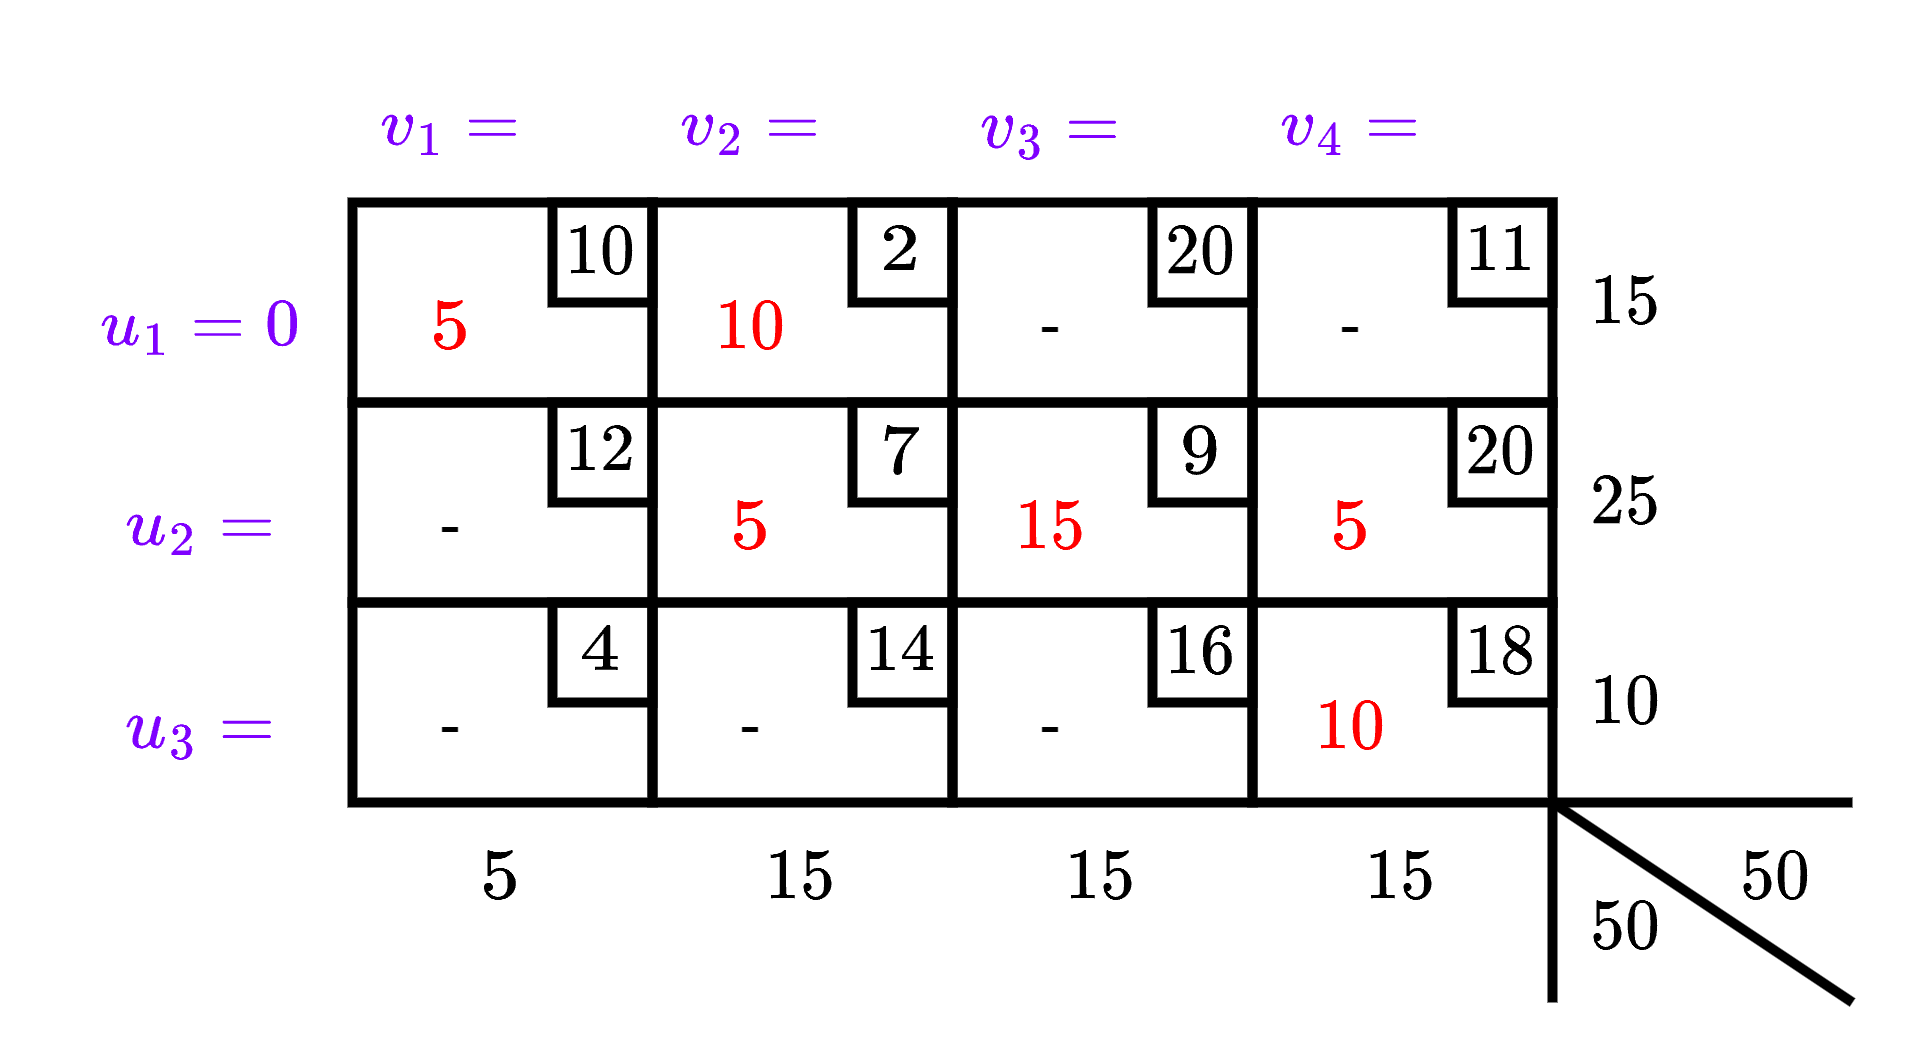
\includegraphics[scale=0.15]{diagram/PTE4-1.png}
        \end{figure}
        \begin{minipage}{0.6\textwidth}
            \begin{figure}[H]
                \centering
                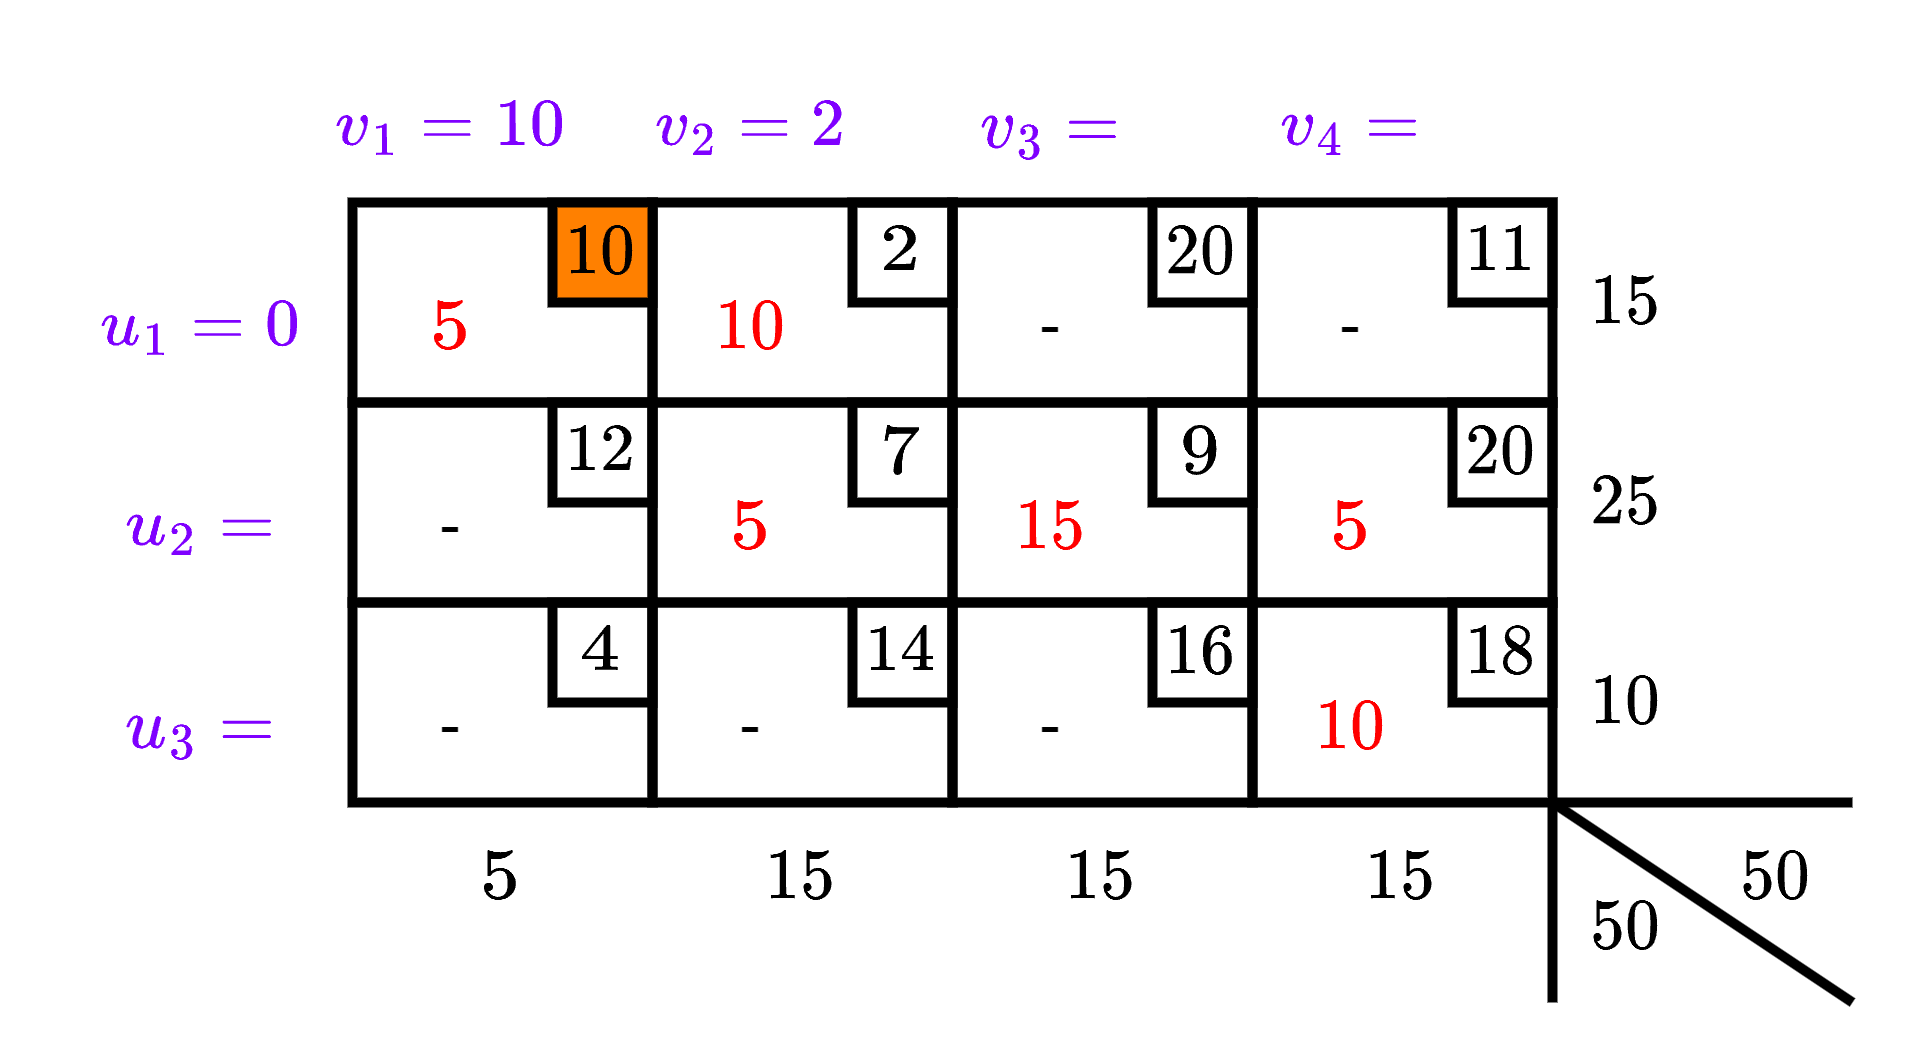
\includegraphics[scale=0.15]{diagram/PTE4-2.png}
            \end{figure}
        \end{minipage}
        \begin{minipage}{0.3\textwidth}
            \begin{equation*}
                v_1 = \colorbox{orange}{10} - 0 = 10
            \end{equation*}
            \begin{equation*}
                v_2 = 2 - 0 = 2
            \end{equation*}
        \end{minipage}
        
        \begin{minipage}{0.6\textwidth}
            \begin{figure}[H]
                \centering
                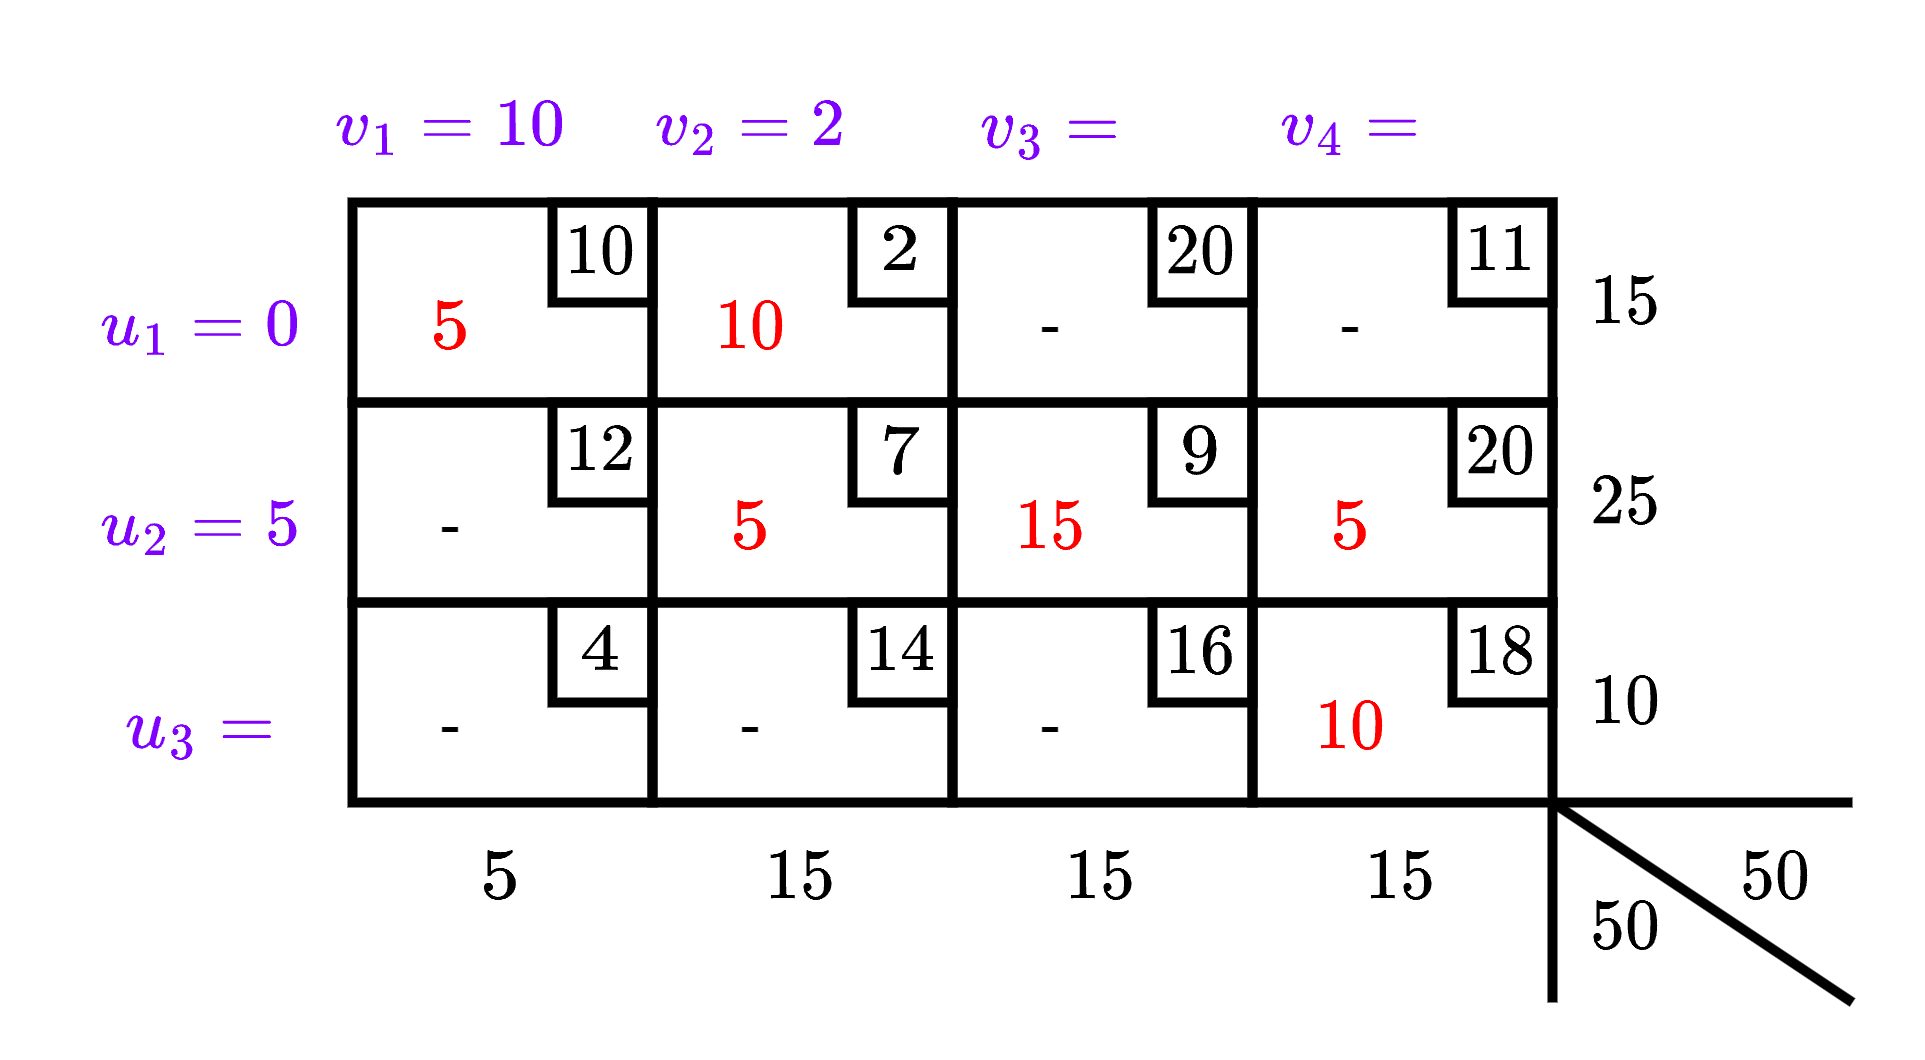
\includegraphics[scale=0.15]{diagram/PTE4-3.png}
            \end{figure}
        \end{minipage}
        \begin{minipage}{0.3\textwidth}
            \begin{equation*}
                u_2 = 7 - 2 = 5
            \end{equation*}
        \end{minipage}

        \begin{figure}[H]
            \centering
            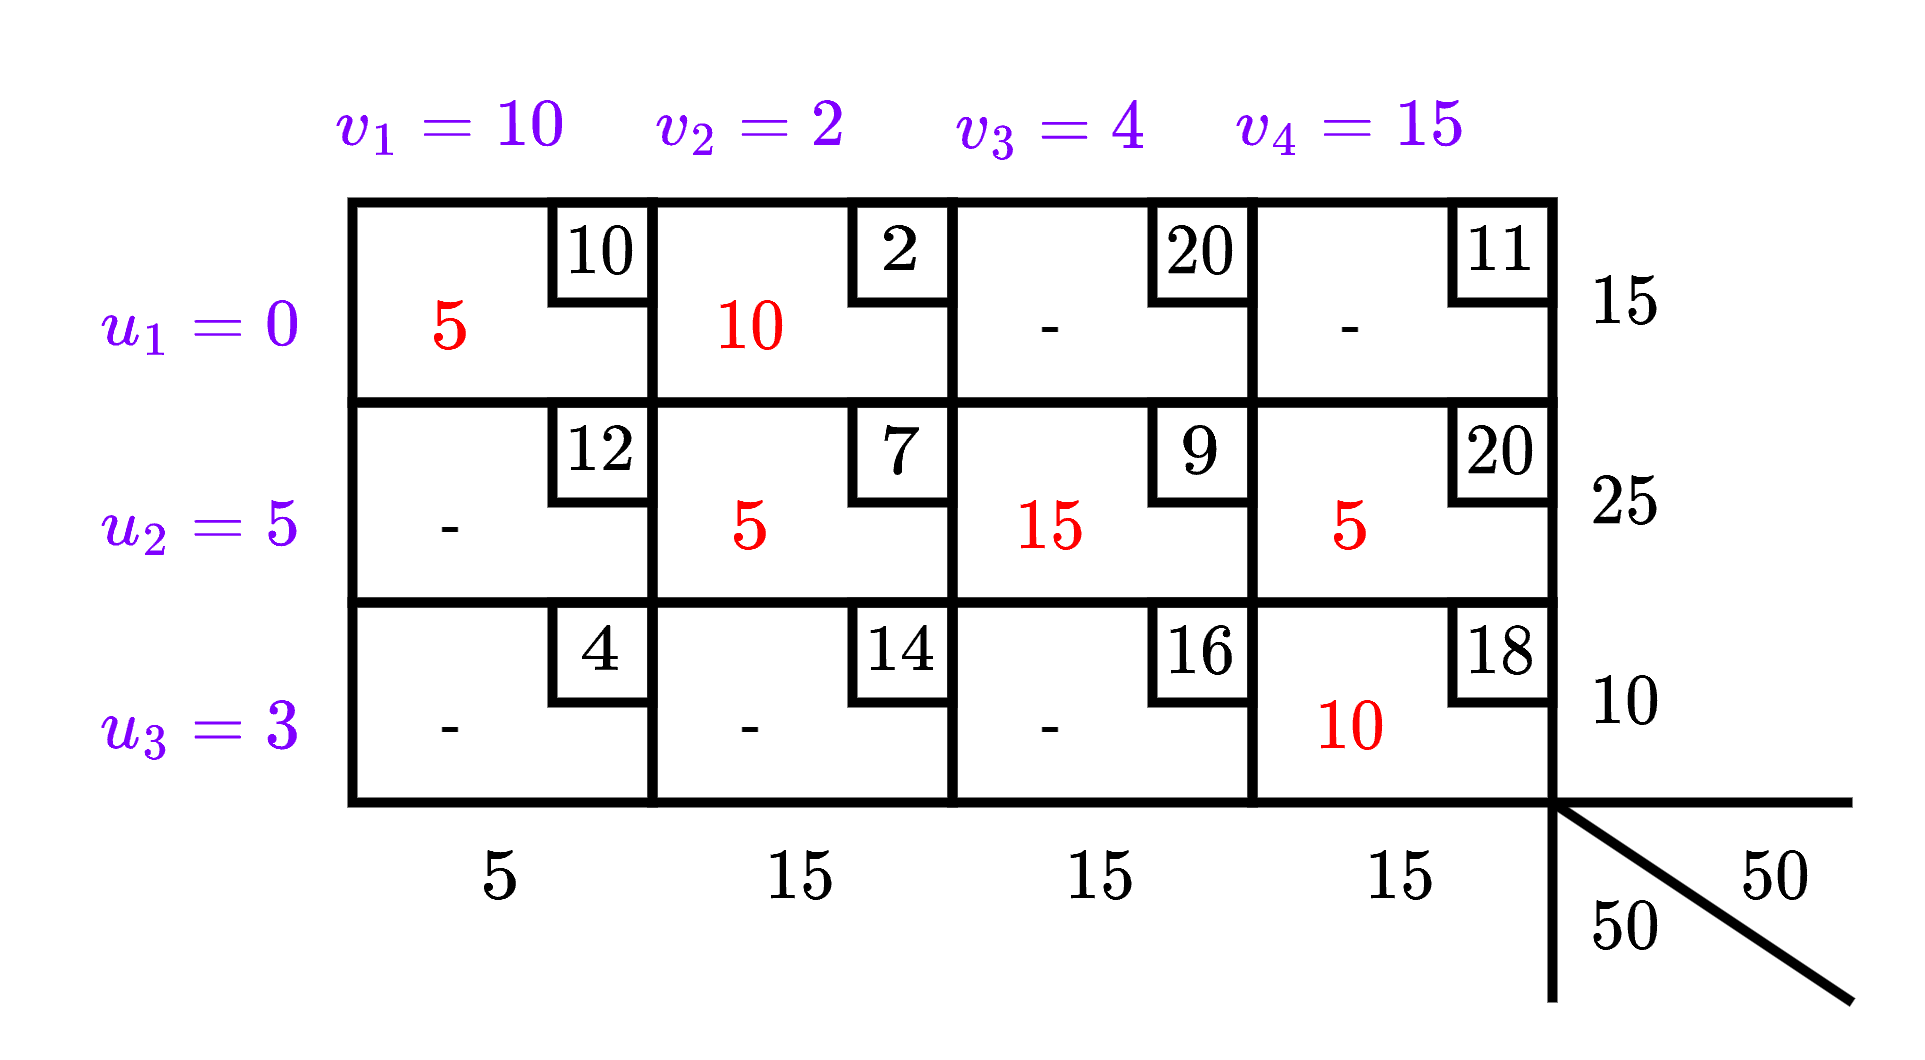
\includegraphics[scale=0.15]{diagram/PTE4-4.png}
        \end{figure}

        \item \textbf{Paso 1.2:} Ahora calculamos los costos reducidos de las celdas que no tienen valor.
        \begin{equation*}
            \overline{C_{ij}} = C_{ij} - u_i - v_j
        \end{equation*}
        \begin{equation*}
            \overline{C_{13}} = \colorbox{orange}{20} - 0 - 4 = \colorbox{yellow}{16}
        \end{equation*}
        \begin{figure}[H]
            \centering
            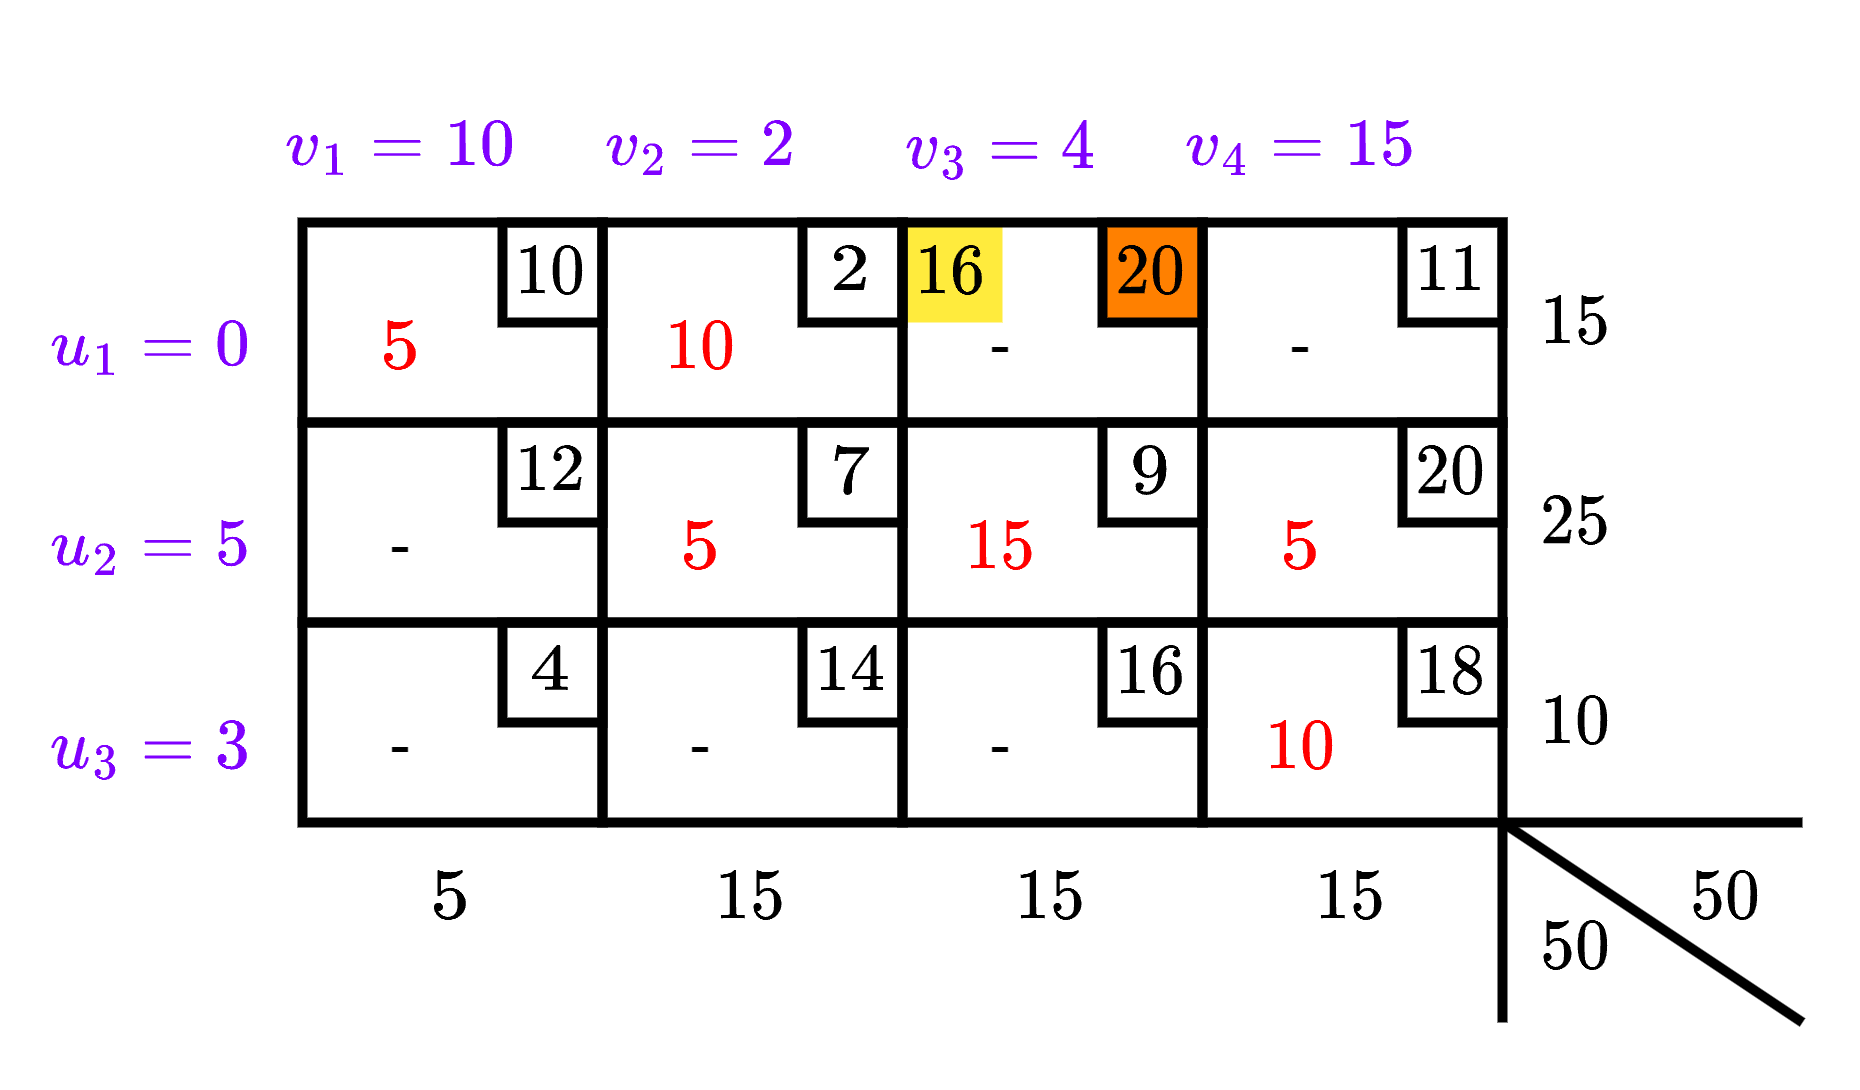
\includegraphics[scale=0.15]{diagram/PTE4-5.png}
        \end{figure}
    \end{itemize}

    \item \textbf{Paso 2:} Verificar si todos los costos reducidos:
    \begin{itemize}
        \item \textbf{Si todos} los costos reducidos son $\geq 0$, entonces hemos llegado a la solución óptima.
        
        \item \textbf{Si existe} uno o varios costos reducidos $\leq 0$, entonces se procede a elegir la celda con el valor más negativo.
        \begin{figure}[H]
            \centering
            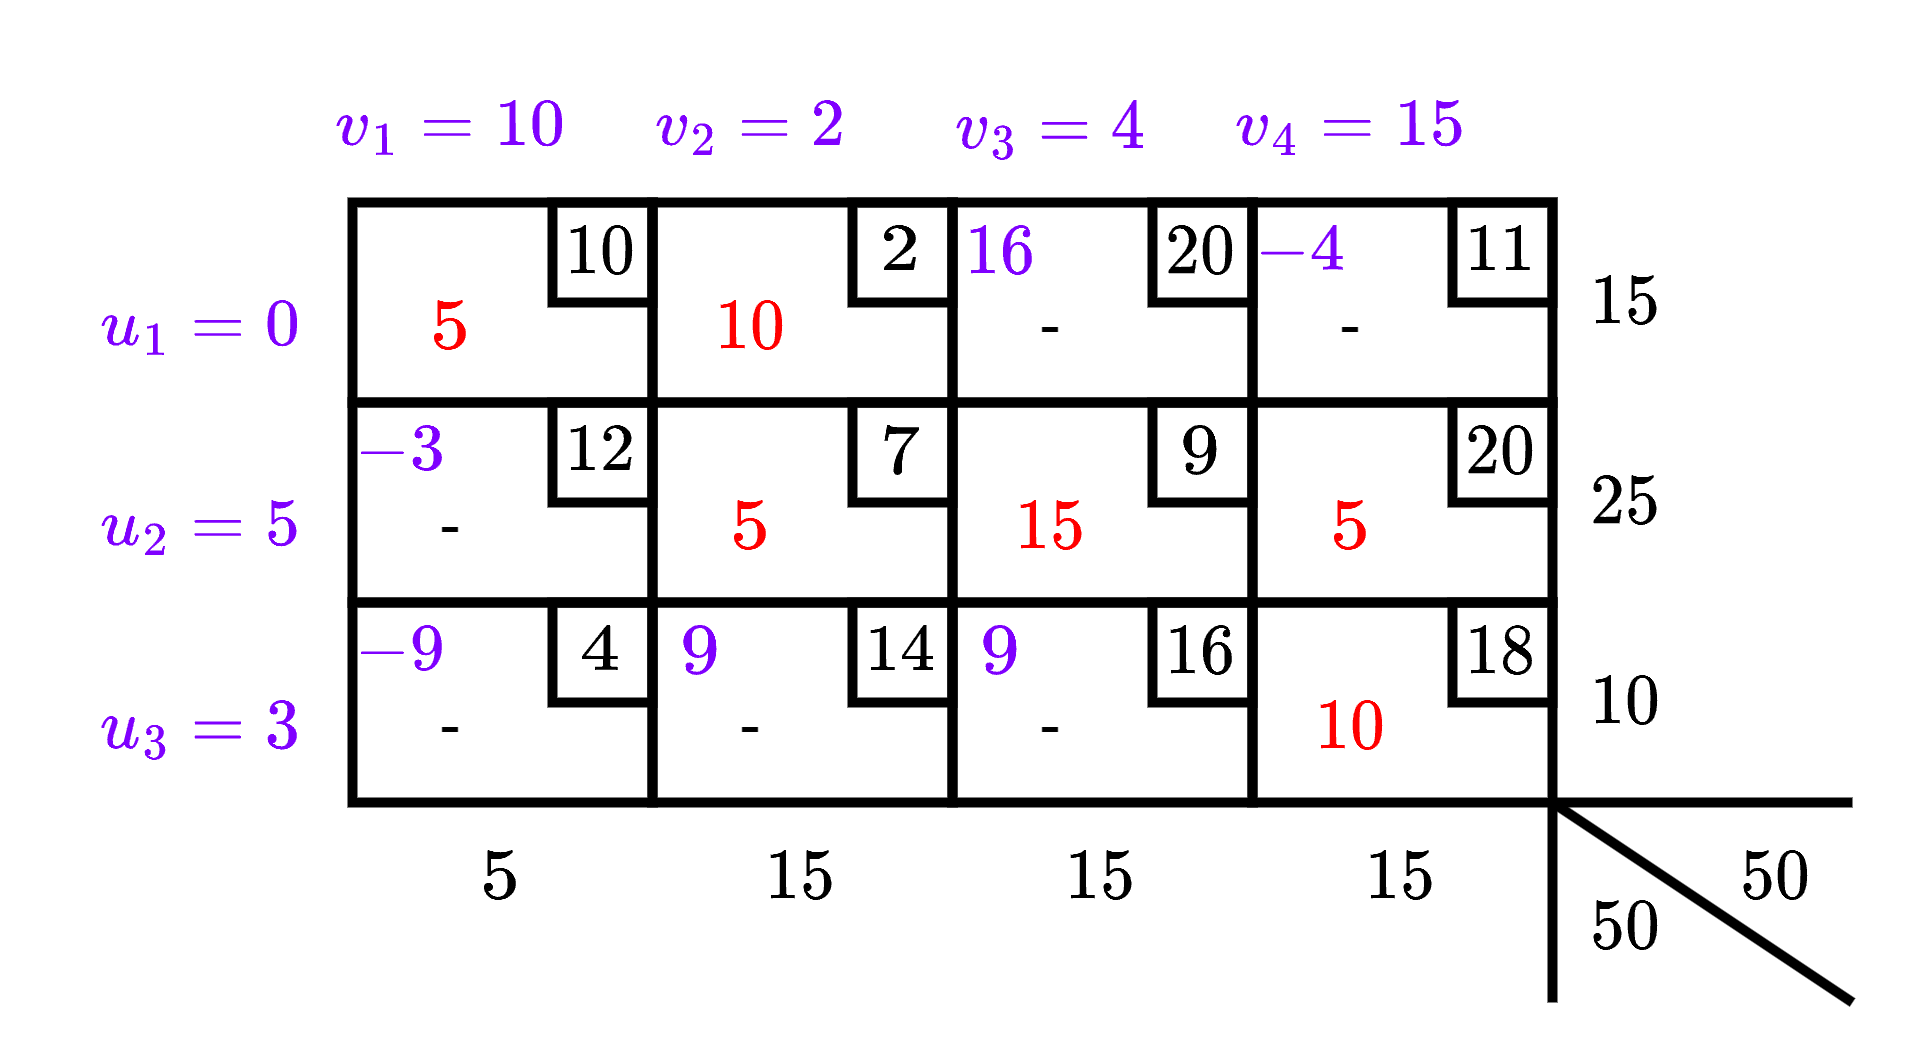
\includegraphics[scale=0.15]{diagram/PTE4-6.png}
        \end{figure}
    \end{itemize}

    \item \textbf{Paso 3:} Elegir la celda con el valor más negativo.
    
    Vemos que la celda $x_{31}$ es el valor más negativo.
    \begin{center}
        $V_{in} = x_{31}$
    \end{center}

    \begin{figure}[H]
        \centering
        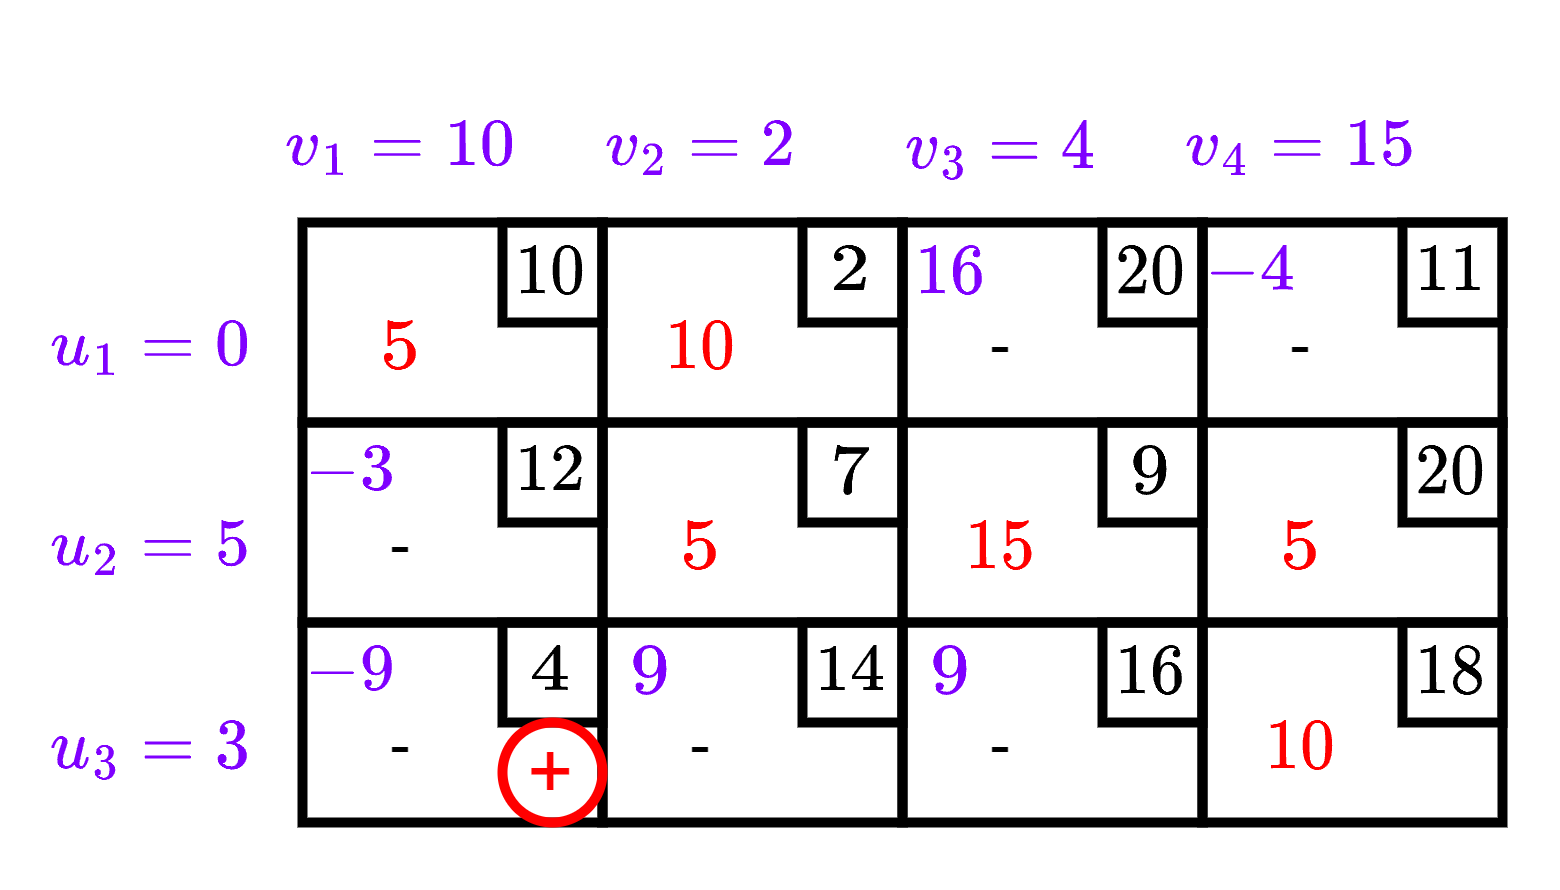
\includegraphics[scale=0.15]{diagram/PTE4-7.png}
    \end{figure}

    \item \textbf{Paso 4:} Utilizamos el método (Stepping-Stone), para actualizar los valores de las celdas y marcar que variable sale.
    \begin{figure}[H]
        \centering
        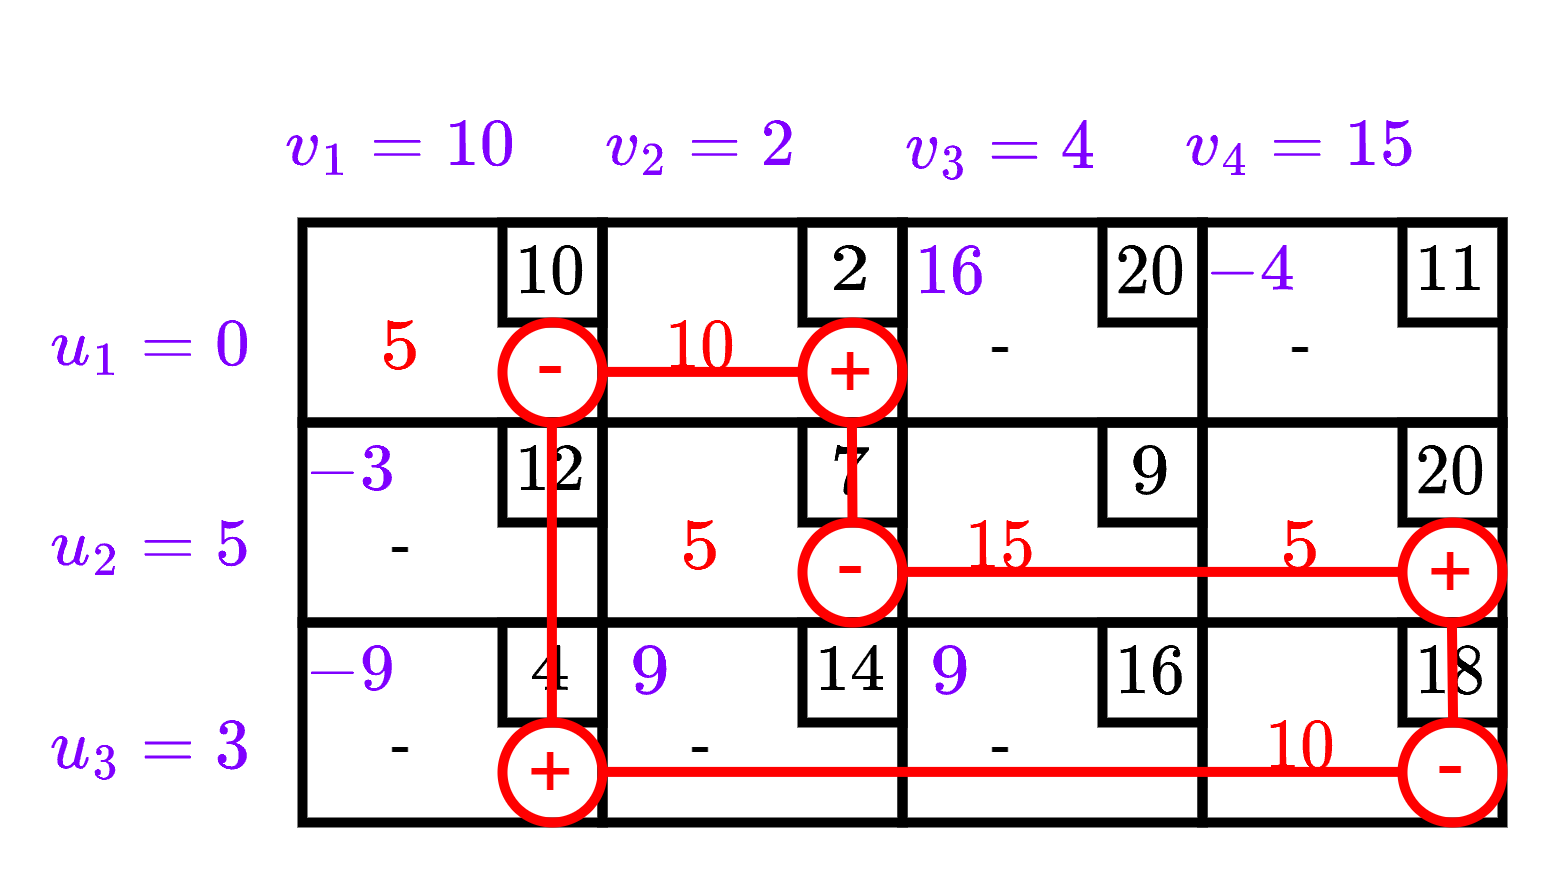
\includegraphics[scale=0.15]{diagram/PTE4-8.png}
    \end{figure}

    \begin{itemize}
        \item \textbf{Paso 4.1:} Elegimos el valor menor de las celdas que se les resta, en este caso tenemos la variables $x_{11}$ y $x_{22}$ con el valor de $5$
        
        Por lo que la variable $x_{11}$ o $x_{22}$ podrian salir.
        \begin{center}
            $V_{out} = x_{22}$
        \end{center}

        Importante: el valor de la variable que sale, se le asigna a la variable que entra.

        \item \textbf{Paso 4.2:} Luego se procede a actualizar los valores de las celdas, sumando o restando el valor de la variable que sale a las celdas con valor.
        \begin{figure}[H]
            \centering
            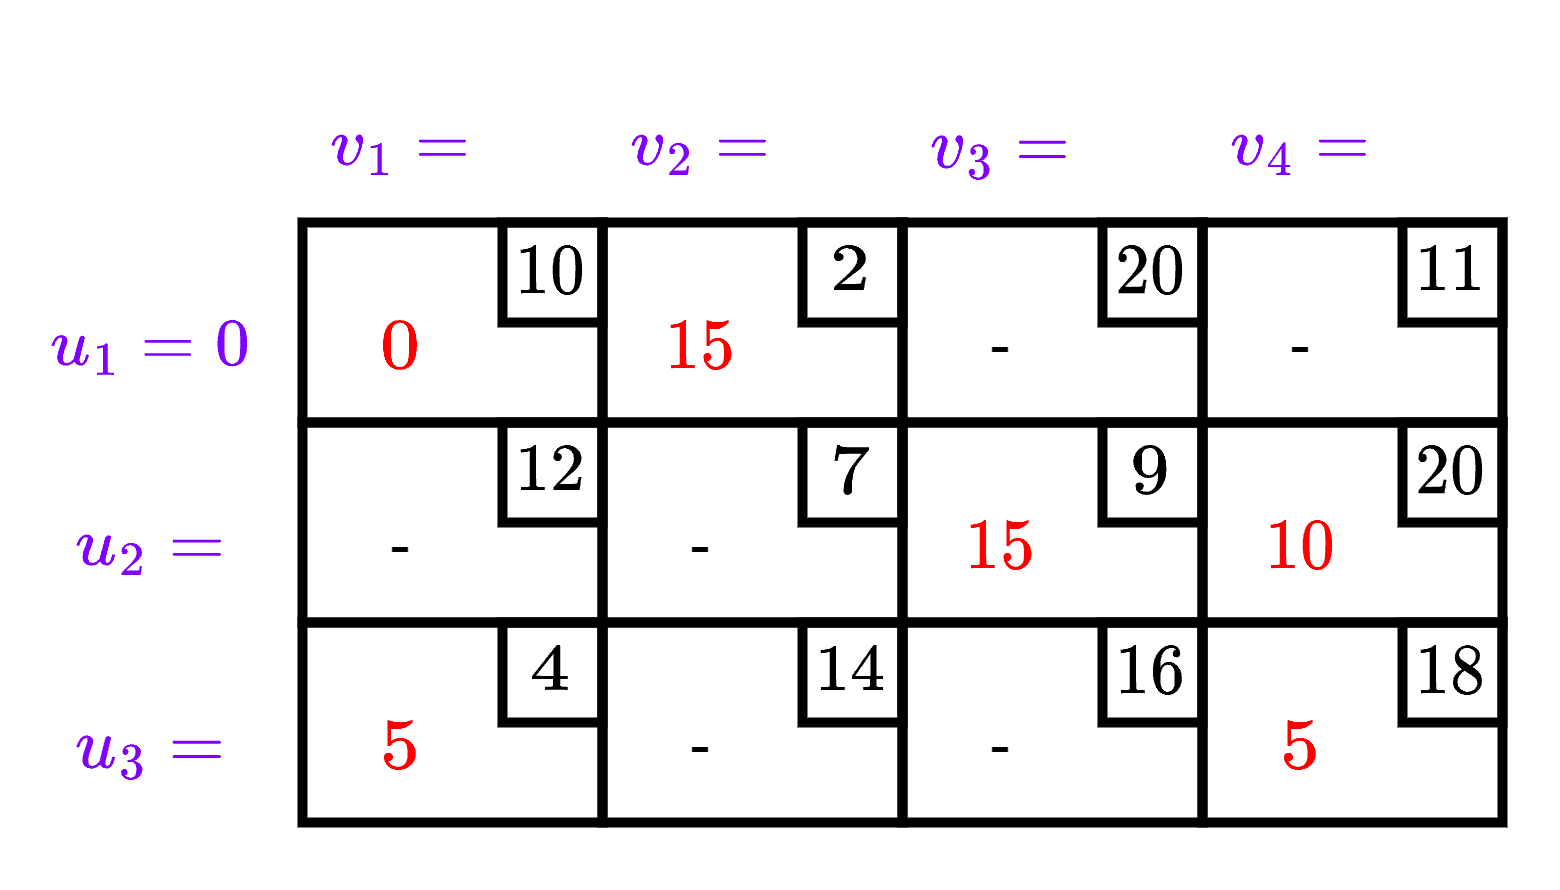
\includegraphics[scale=0.15]{diagram/PTE4-9.png}
        \end{figure}
        \begin{align*}
            Z &= 0 \cdot 10 + 15 \cdot 2 + 15 \cdot 9 + 10 \cdot 20 + 5 \cdot 4 + 5 \cdot 18\\
            &= 0 + 30 + 135 + 200 + 20 + 90 \\
            &= 475
        \end{align*}
    \end{itemize}
    \item \textbf{Paso ?:} Repetir los pasos hasta que en el paso 2 todos los costos reducidos sean $\geq 0$.
    \begin{figure}[H]
        \centering
        \includegraphics[scale=0.15]{diagram/PTE4-10.png}
    \end{figure}

    \begin{figure}[H]
        \centering
        \includegraphics[scale=0.15]{diagram/PTE4-11.png}
    \end{figure}
    \begin{align*}
        Z &= 15 \cdot 2 + 0 \cdot 11 + 15 \cdot 9 + 10 \cdot 20 + 5 \cdot 4 + 5 \cdot 18\\
        &= 30 + 0 + 135 + 200 + 20 + 90 \\
        &= 475
    \end{align*}

    \begin{figure}[H]
        \centering
        \includegraphics[scale=0.15]{diagram/PTE4-12.png}
    \end{figure}

    \begin{figure}[H]
        \centering
        \includegraphics[scale=0.15]{diagram/PTE4-13.png}
    \end{figure}

    \begin{figure}[H]
        \centering
        \includegraphics[scale=0.15]{diagram/PTE4-14.png}
    \end{figure}

    \item Calculamos el valor de la función objetivo.
    \begin{align*}
        Z &= 5 \cdot 2 + 10 \cdot 11 + 10 \cdot 7 + 15 \cdot 9 + 5 \cdot 4 + 5 \cdot 18\\
        &= 10 + 110 + 70 + 135 + 20 + 90 \\
        &= 435
    \end{align*}
\end{itemize}

\newpage
\subsection*{Problema 14: Repaso P.T.}
Escribir el M.L. para el siguiente P.T.:
\begin{figure}[H]
    \centering
    \includegraphics[scale=0.15]{diagram/PTE5.png}
\end{figure}

\subsubsection*{Por Regla Nor-Oeste}
\begin{figure}[H]
    \centering
    \includegraphics[scale=0.15]{diagram/PTE5-1.png}
\end{figure}

\subsubsection*{Utilizando los criterios:}
\begin{figure}[H]
    \centering
    \includegraphics[scale=0.15]{diagram/PTE5-2.png}
\end{figure}
\begin{align*}
    Z &= 7 \cdot 10 + 1 \cdot 4 + 5 \cdot 3 + 0 \cdot 4 + 6 \cdot 0 \\
    &= 70 + 4 + 15 + 0 + 0 \\
    &=  89
\end{align*}

\begin{figure}[H]
    \centering
    \includegraphics[scale=0.15]{diagram/PTE5-3.png}
\end{figure}
\begin{align*}
    Z &= 2 \cdot 10 + 6 \cdot 4 + 5 \cdot 2 + 0 \cdot 4 + 6 \cdot 0 \\
    &= 20 + 24 + 10 + 0 + 0 \\
    &=  54
\end{align*}

\begin{figure}[H]
    \centering
    \includegraphics[scale=0.15]{diagram/PTE5-4.png}
\end{figure}
\begin{align*}
    Z &= 2 \cdot 10 + 6 \cdot 4 + 0 \cdot 2 + 5 \cdot 2 + 6 \cdot 0 \\
    &= 20 + 24 + 0 + 10 + 0 \\
    &=  54
\end{align*}
\begin{figure}[H]
    \centering
    \includegraphics[scale=0.15]{diagram/PTE5-5.png}
\end{figure}
\begin{align*}
    Z &= 6 \cdot 4 + 2 \cdot 2 + 5 \cdot 2 + 2 \cdot 1 + 4 \cdot 0 \\
    &= 24 + 4 + 10 + 2 + 0 \\
    &=  40
\end{align*}
\end{document}